
\chapter{Thermohaline overturning circulation}
\label{ch:thermohaline}

%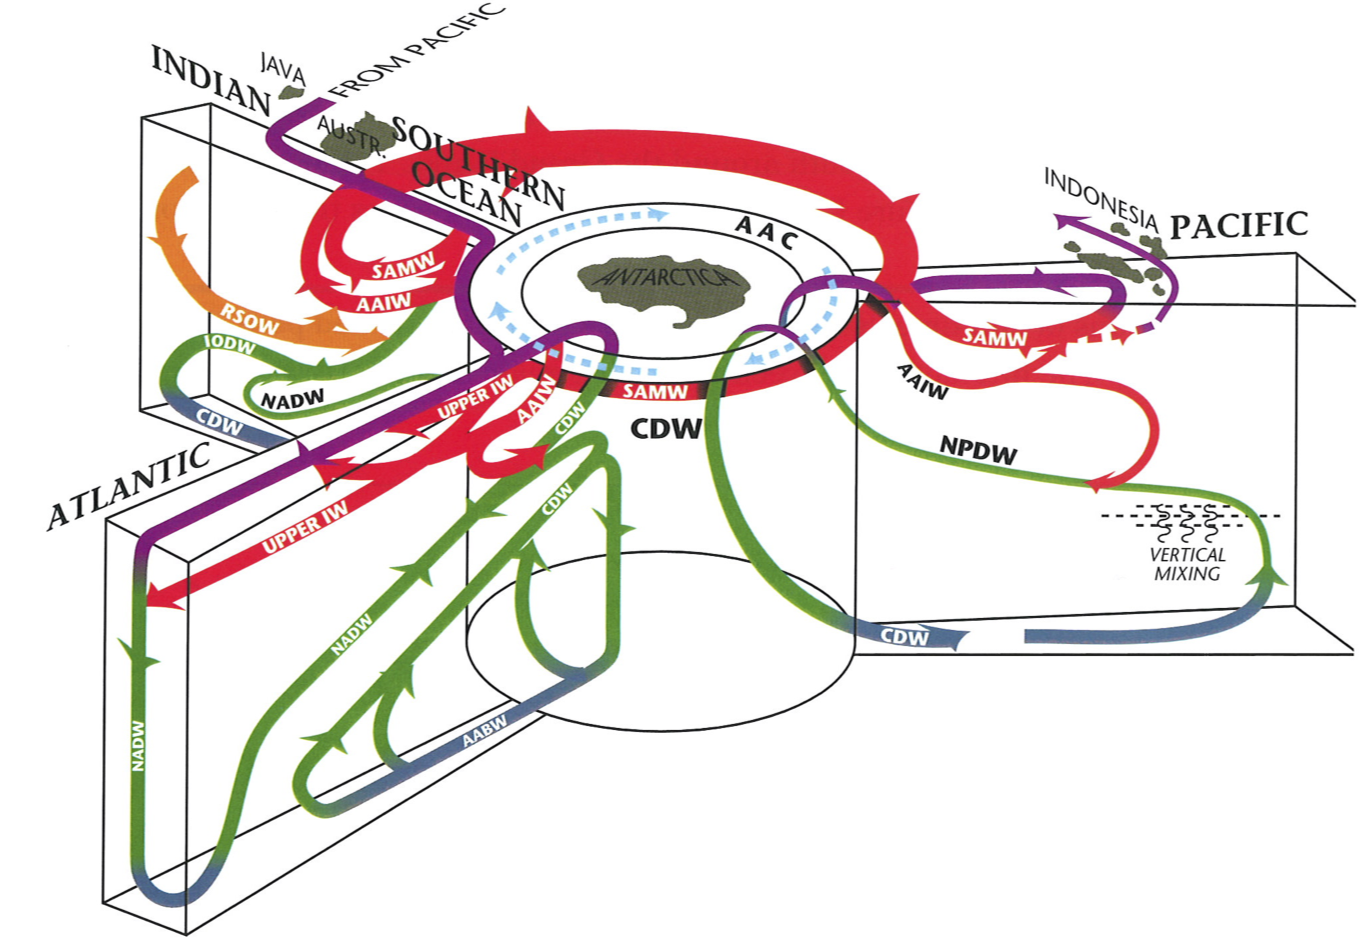
\includegraphics[width=6in]{figs/WaterMasses/Schmitz96Fig91.png}
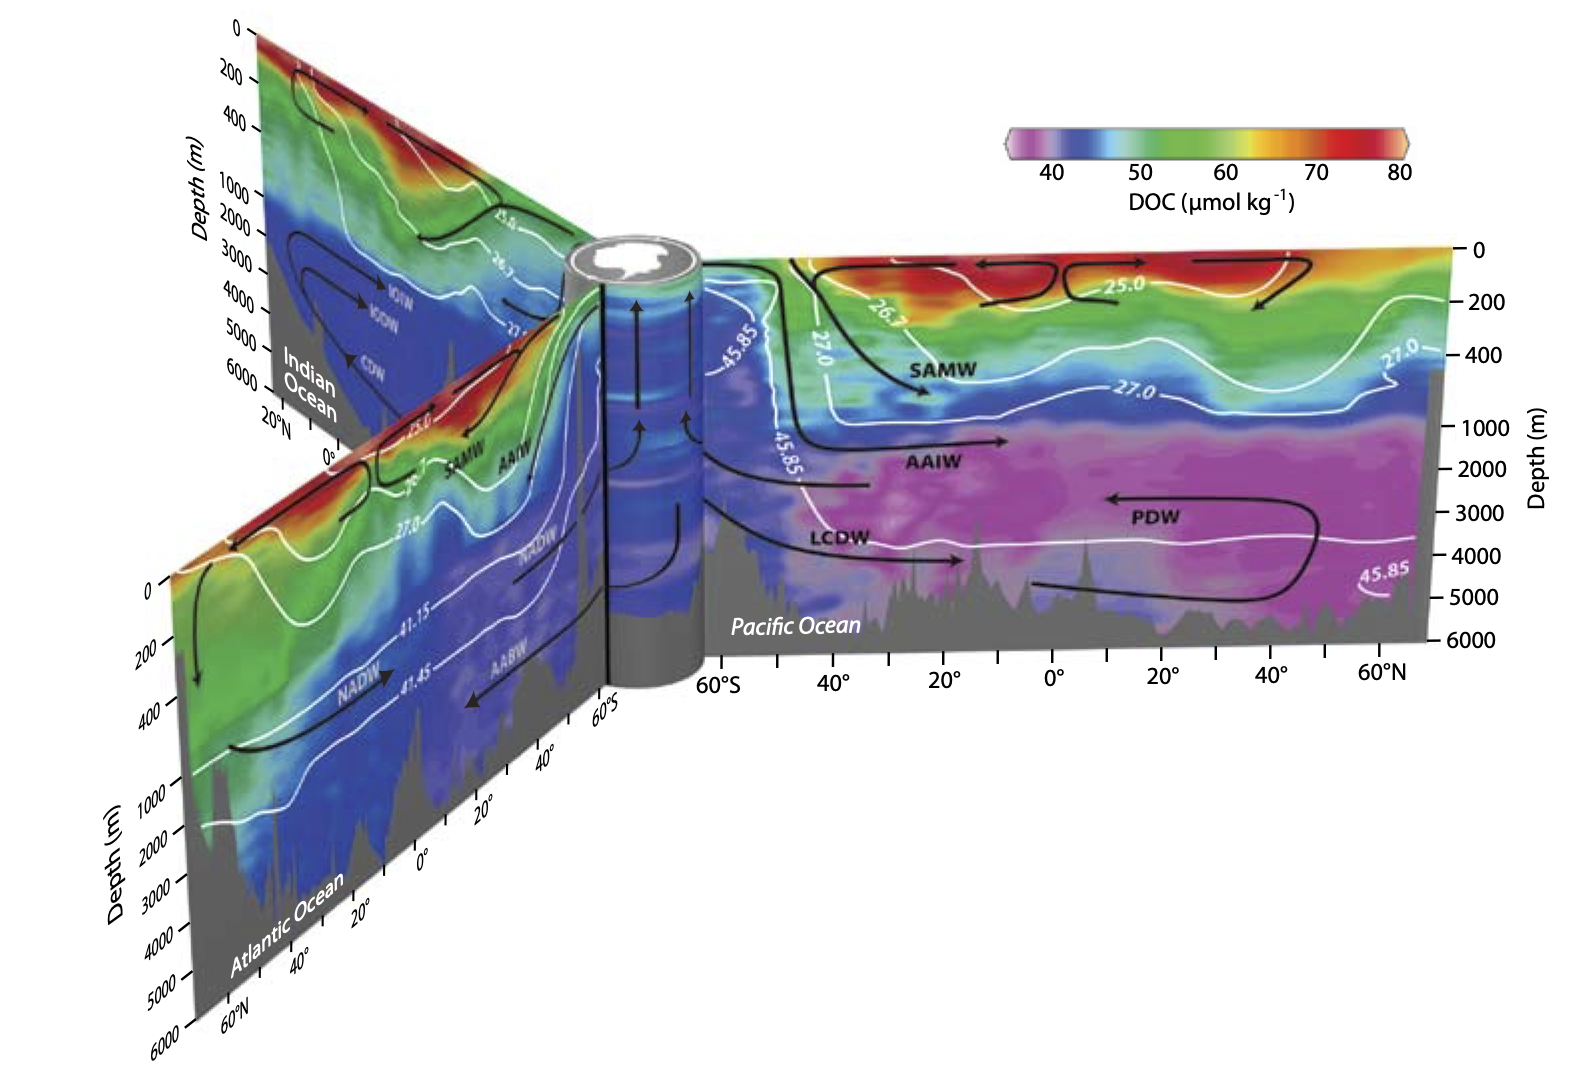
\includegraphics[width=6in]{figs/WaterMasses/HansellEtAl09.png}


The water masses we saw in the previous chapter are the result of water formation at the ocean's surface, and for those that make it to depth, sinking of water.  From the picture in \fref{fig:AnnotateSections}a it is very evocative of the idea that dense water is created in the Southern Ocean and then sinks along the bottom to the north and fills the bottom basin of the Pacific.  However, if that sinking of cold salty water happens all the time (and evidence is that it does), then there are  two choices for where that water ends up eventually.  The deep ocean could fill up with cold, salty water, or heat and fresh water can mix from above and modify it.  

We sketch this here, where the $1.1^oC$ isotherm is highlighted (\fref{fig:AnnotatePacific}.  The dense water flows counter clockwise in this sketch, and must cross isotherms in order to complete the closed circuit.  If water crosses an isotherm, it must warm, and the only way for this to happen is by vertical mixing.  This chapter discusses this circulation, the evidence for it, and the mechanisms that drive it.

\begin{figure}[hbt]
  \begin{center}
    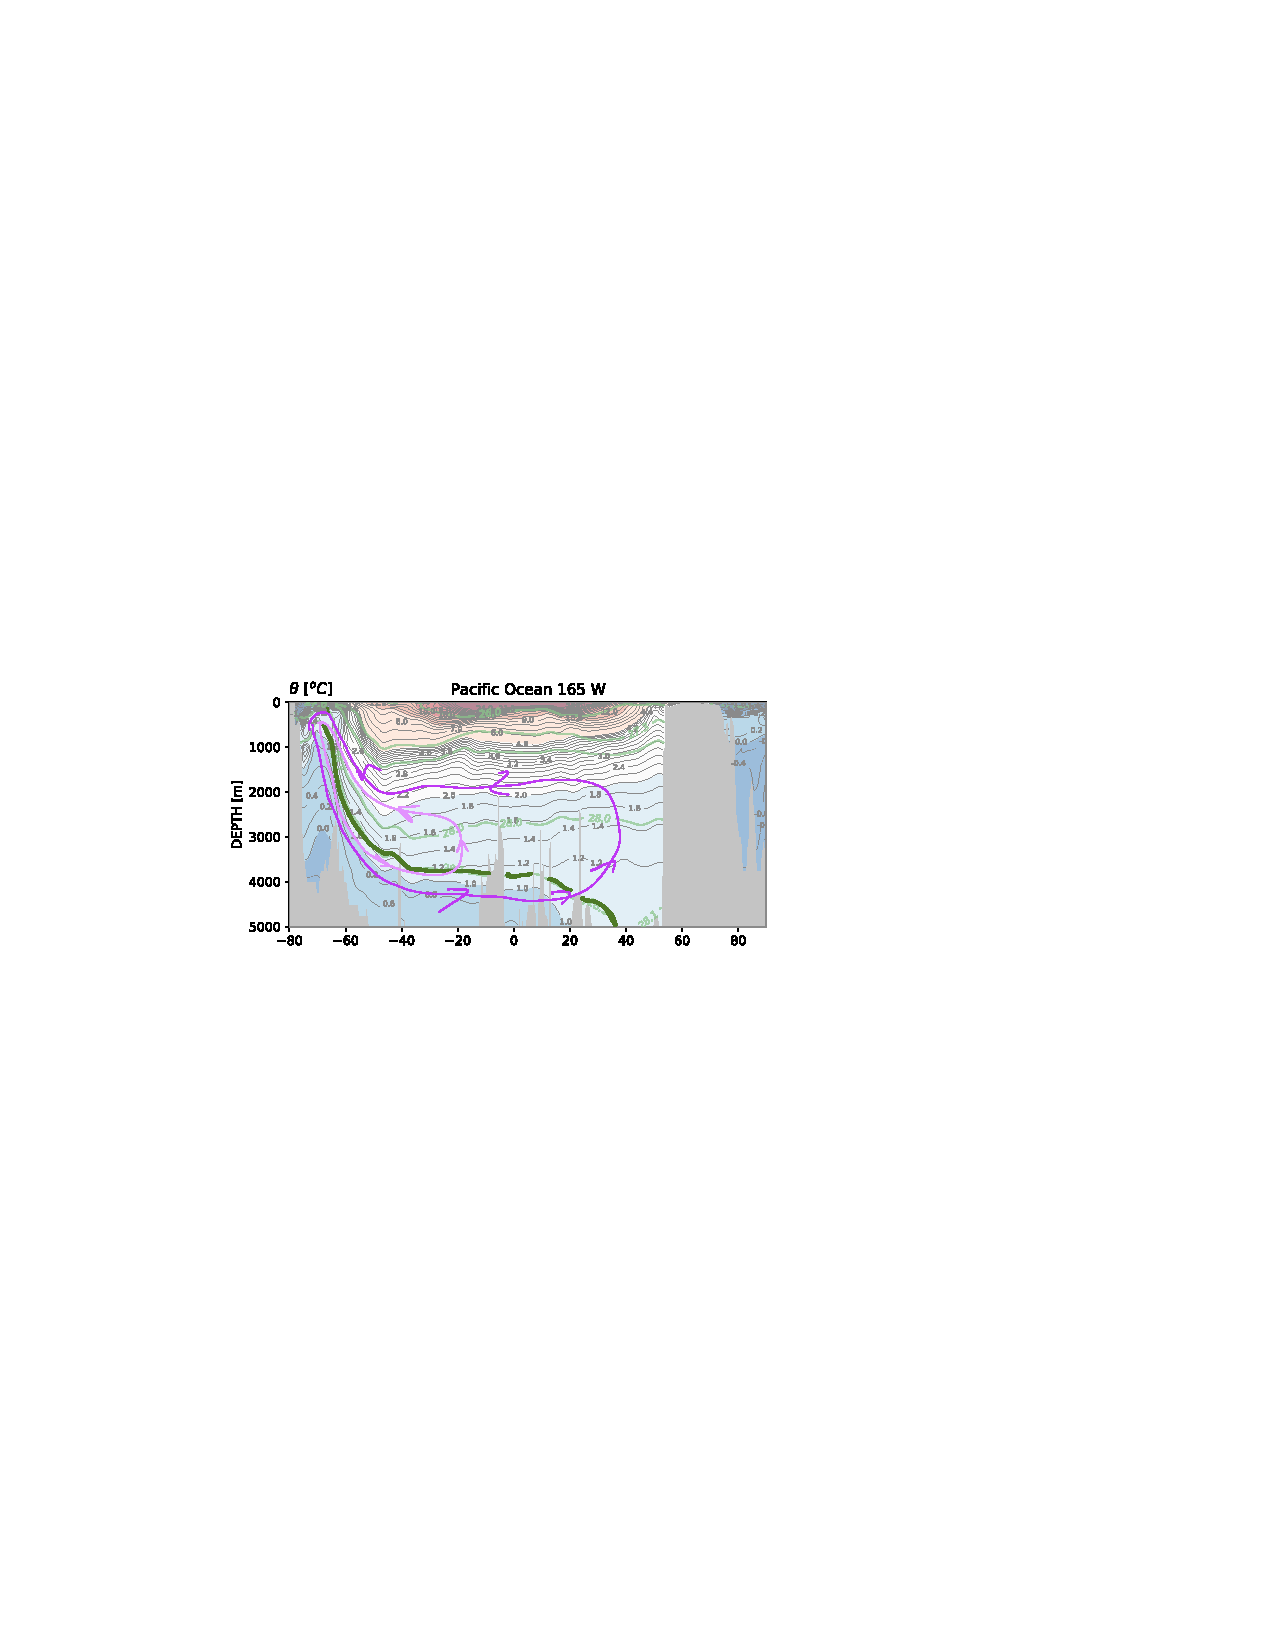
\includegraphics{figs/WaterMasses/AnnotatePacific}
    \caption{Sketch of deep overturning circulation in the Pacific.  Green contour is the 1.1 degree-C isotherm (approximately) and the purple lines are idealized paths taken by the water.}
    \label{fig:AnnotatePacific}  
  \end{center}
\end{figure}



\section{Inferring the overturning circulation from other tracers}

\subsection{Bio-active tracers}

The physical tracers like temperature and salinity are \emph{conservative} in that they cannot be destroyed or consumed in the water column.  This is not the case with bio-active tracers which change as the water is exposed to biological activity.   In general, the upper ocean where sunlight can penetrate is dominated by photosynthesis, where plants, largely phytoplankton,  convert CO2 and nutrients to Oxygen.  Outside the euphotic zone, the ocean is dominated by respiration, where animals and bacteria consume oxygen and respire CO2.  This leads to the general picture in \fref{fig:P16BioActive}.  The youngest water near the surface is high in O2 and low in CO2 and nutrients like Nitrate and Silica.  The Antarctic Intermediate water is a clear plume of high-O2 water being pushed south under the subtropical gyre.  The Antarctic bottom water is seen pouring into the  Pacific and losing oxygen as it moves north and gaining CO2.  The lowest oxygen and highest CO2 are found at around 1000 m in the north Pacific. Based on this logic alone we might argue that the oldest water is where this oxygen minimum is.  That would not quite be correct - the oldest water is thought to be about 1000 m deeper (see the next section), and that is because the net respiration rate tends to decrease with depth.    

Nitrate and Silica are also highest at this point, though the have maxima at slightly different depths.  Nutrients accumulate in the water column largely due to sinking of particles from the near-surface ocean. The particles that have large silica content like shells and bones tend to sink deeper than more labile material (bodies, fecal pellets) that contains significant nitrate.  So, similarly to oxygen, the minimima and maxima of the nutrients gives the correct sense of water sinking in the Southern Ocean and rising in the North Pacific, but the details depend on biological processes.  

If we knew the rate of oxygen consumption, or the rate of particle fluxes in the deep ocean, we could use this information to estimate the strength of the overturning circulation.  So if  this rate were on average c umol/kg/day, and there is 200 umol/kg difference between the AABW oxygen content and the oxygen minimum in the north Pacific, we could make an estimate of how many days it would take for the water to get to that minimum.  Unfortunately, for most of the biological tracers, the consumption/production rates are poorly constrained, and understood to be spatially variable, so this approach is not typically used.  

\begin{figure}[hbt]
  \begin{center}
    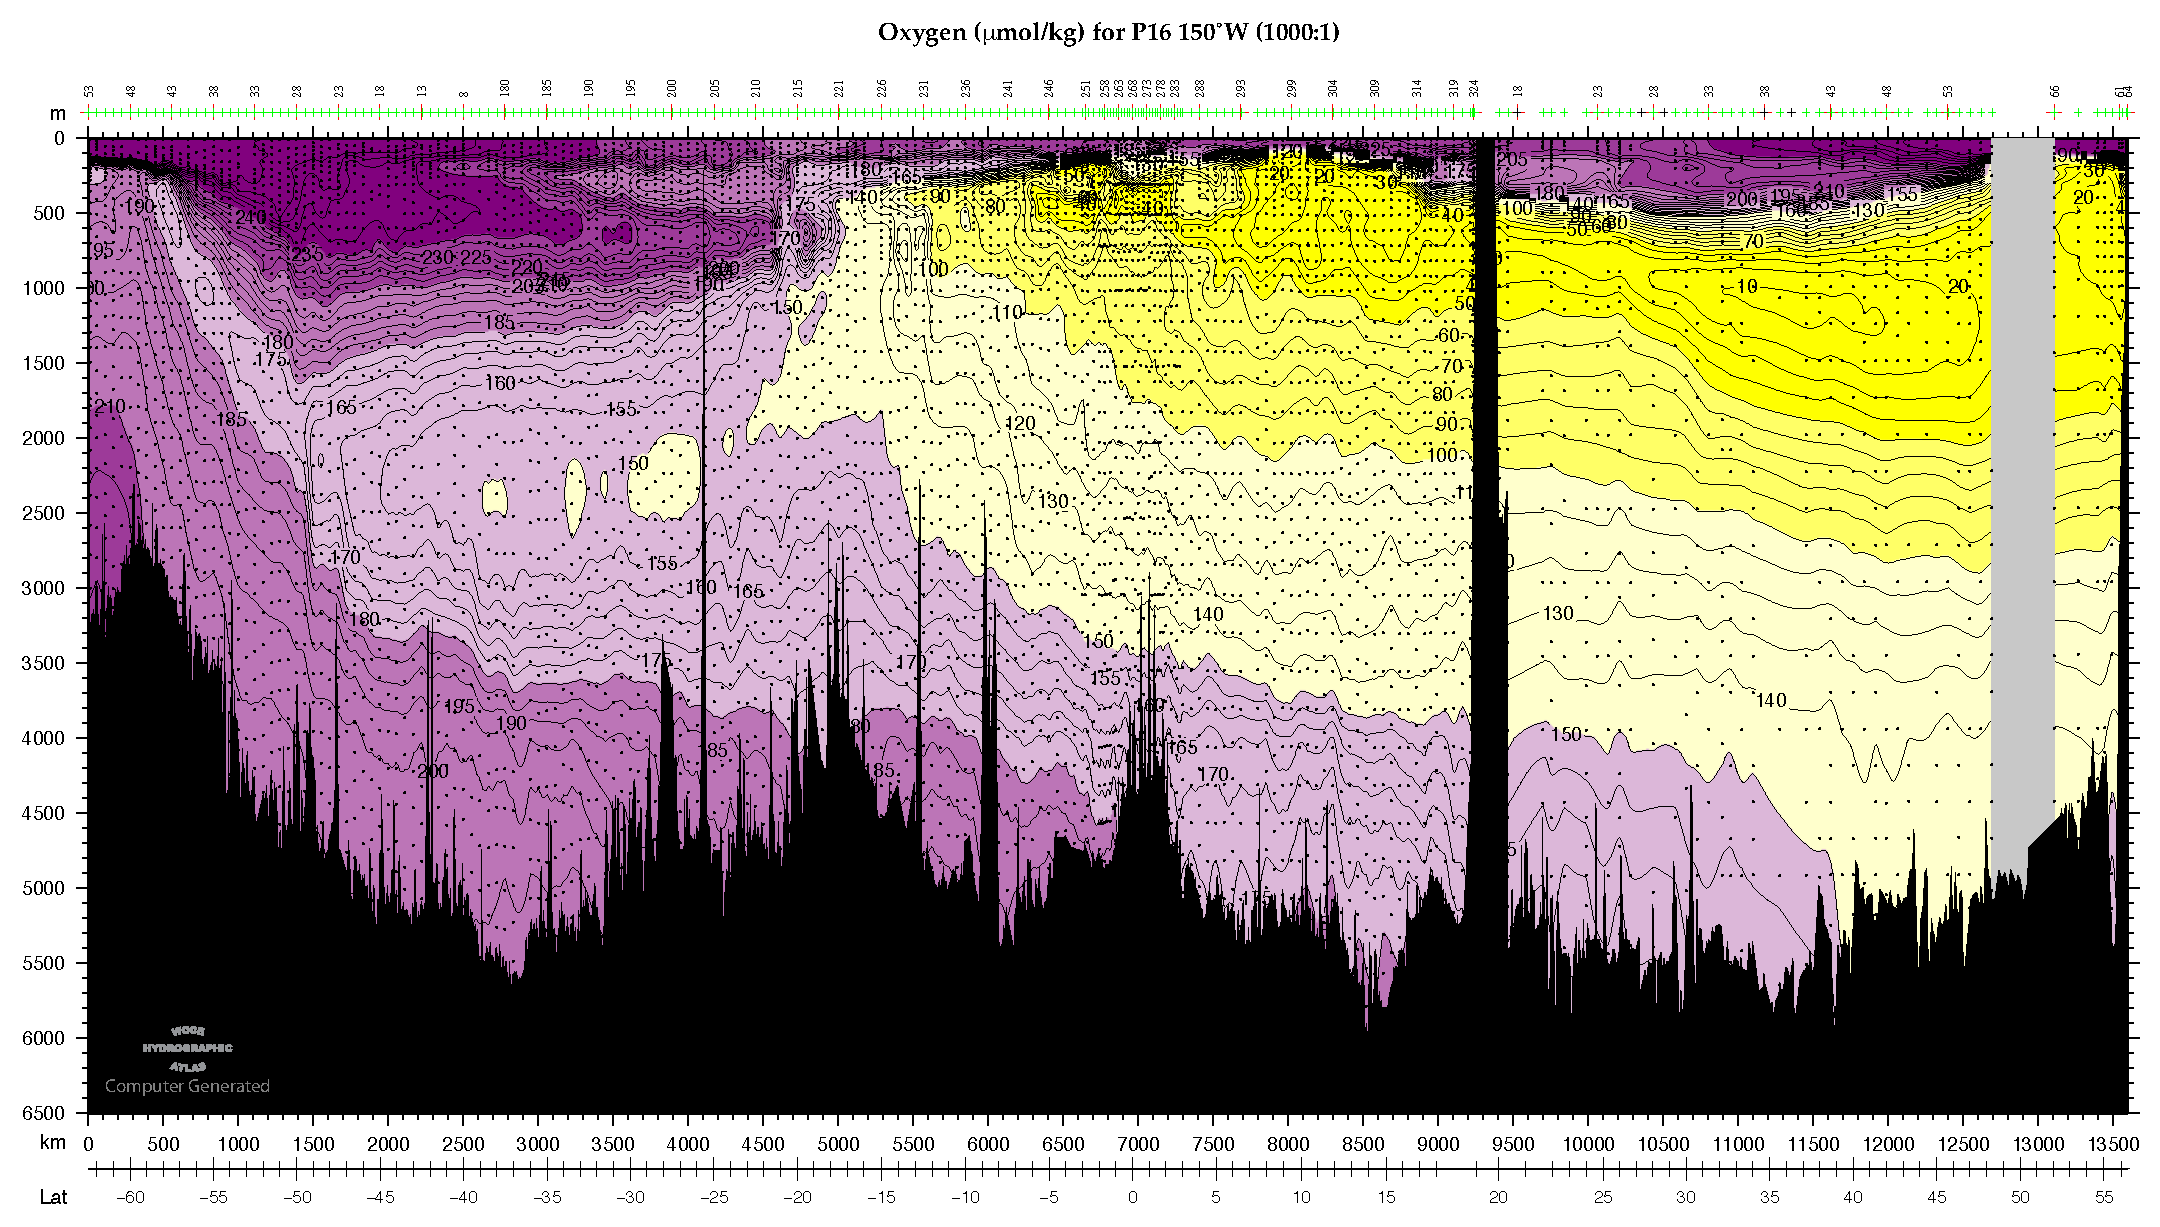
\includegraphics{figs/WaterMasses/P16OxygenCrop}
    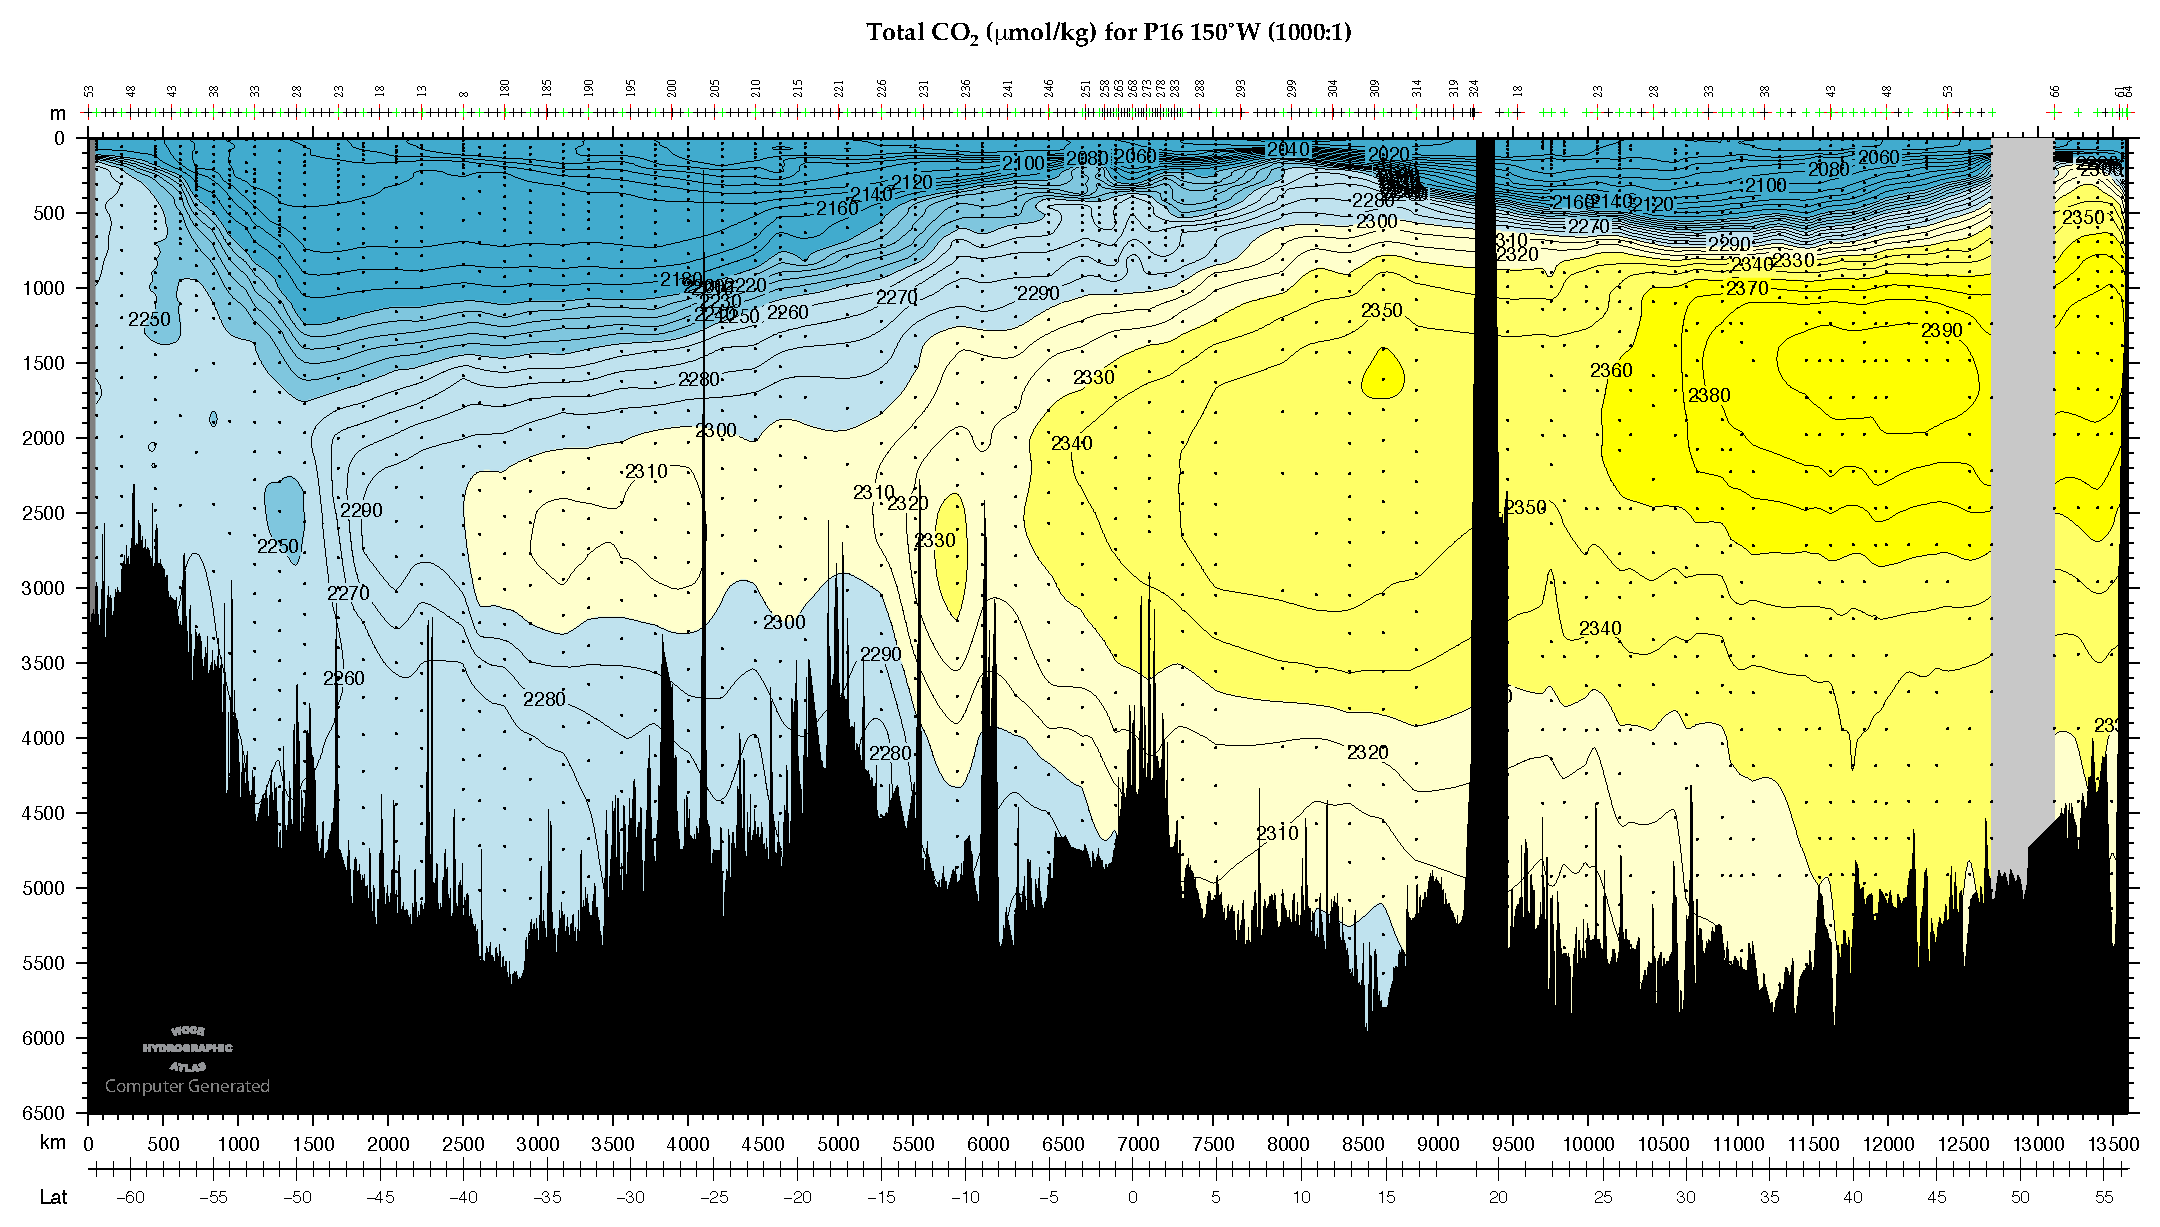
\includegraphics{figs/WaterMasses/P16CO2Crop}
    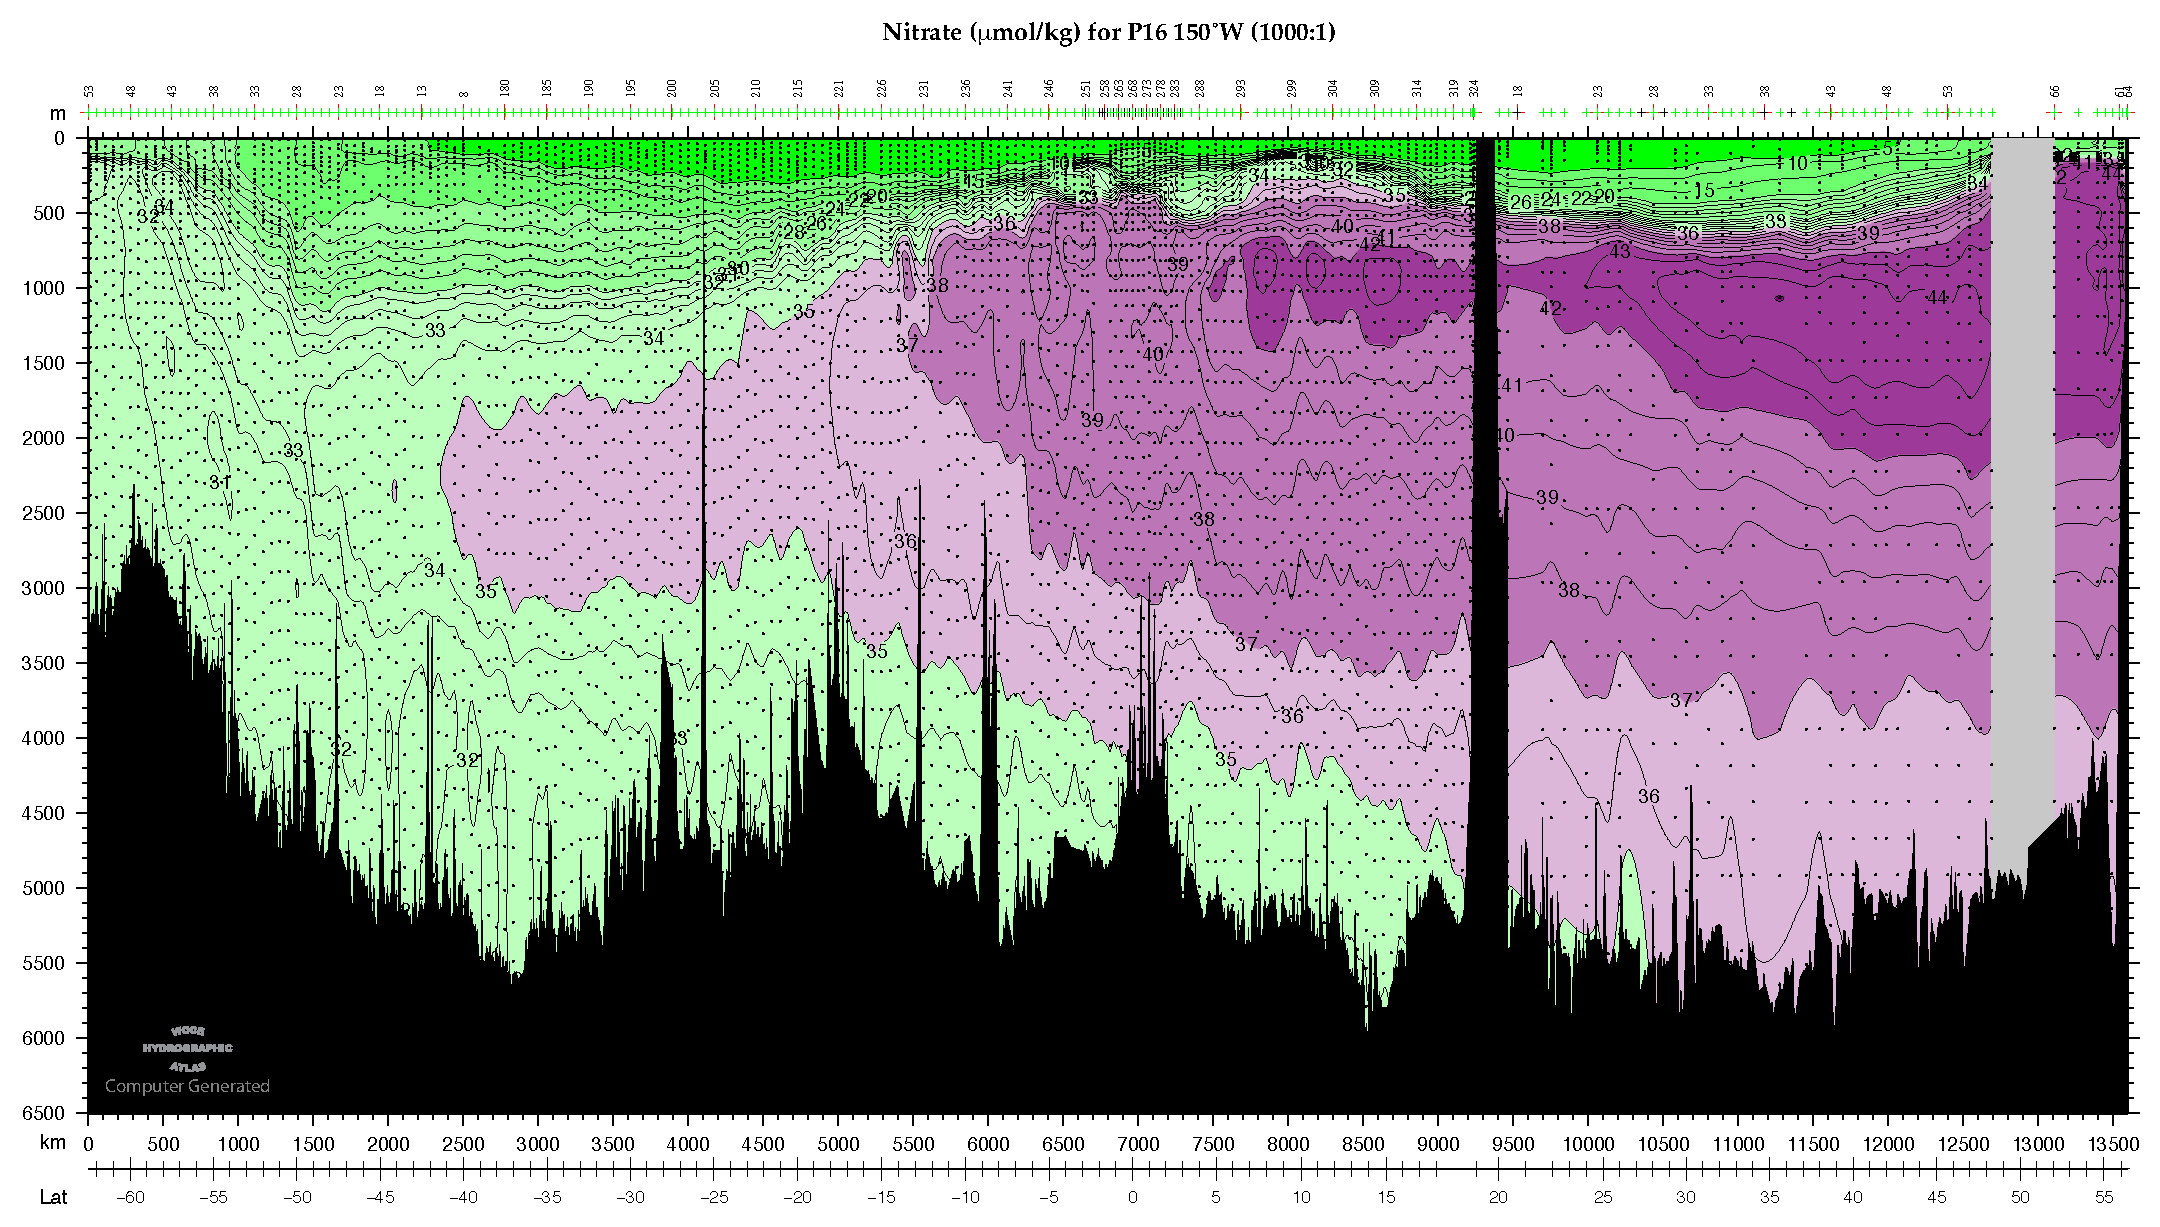
\includegraphics{figs/WaterMasses/P16NitrateCrop}
    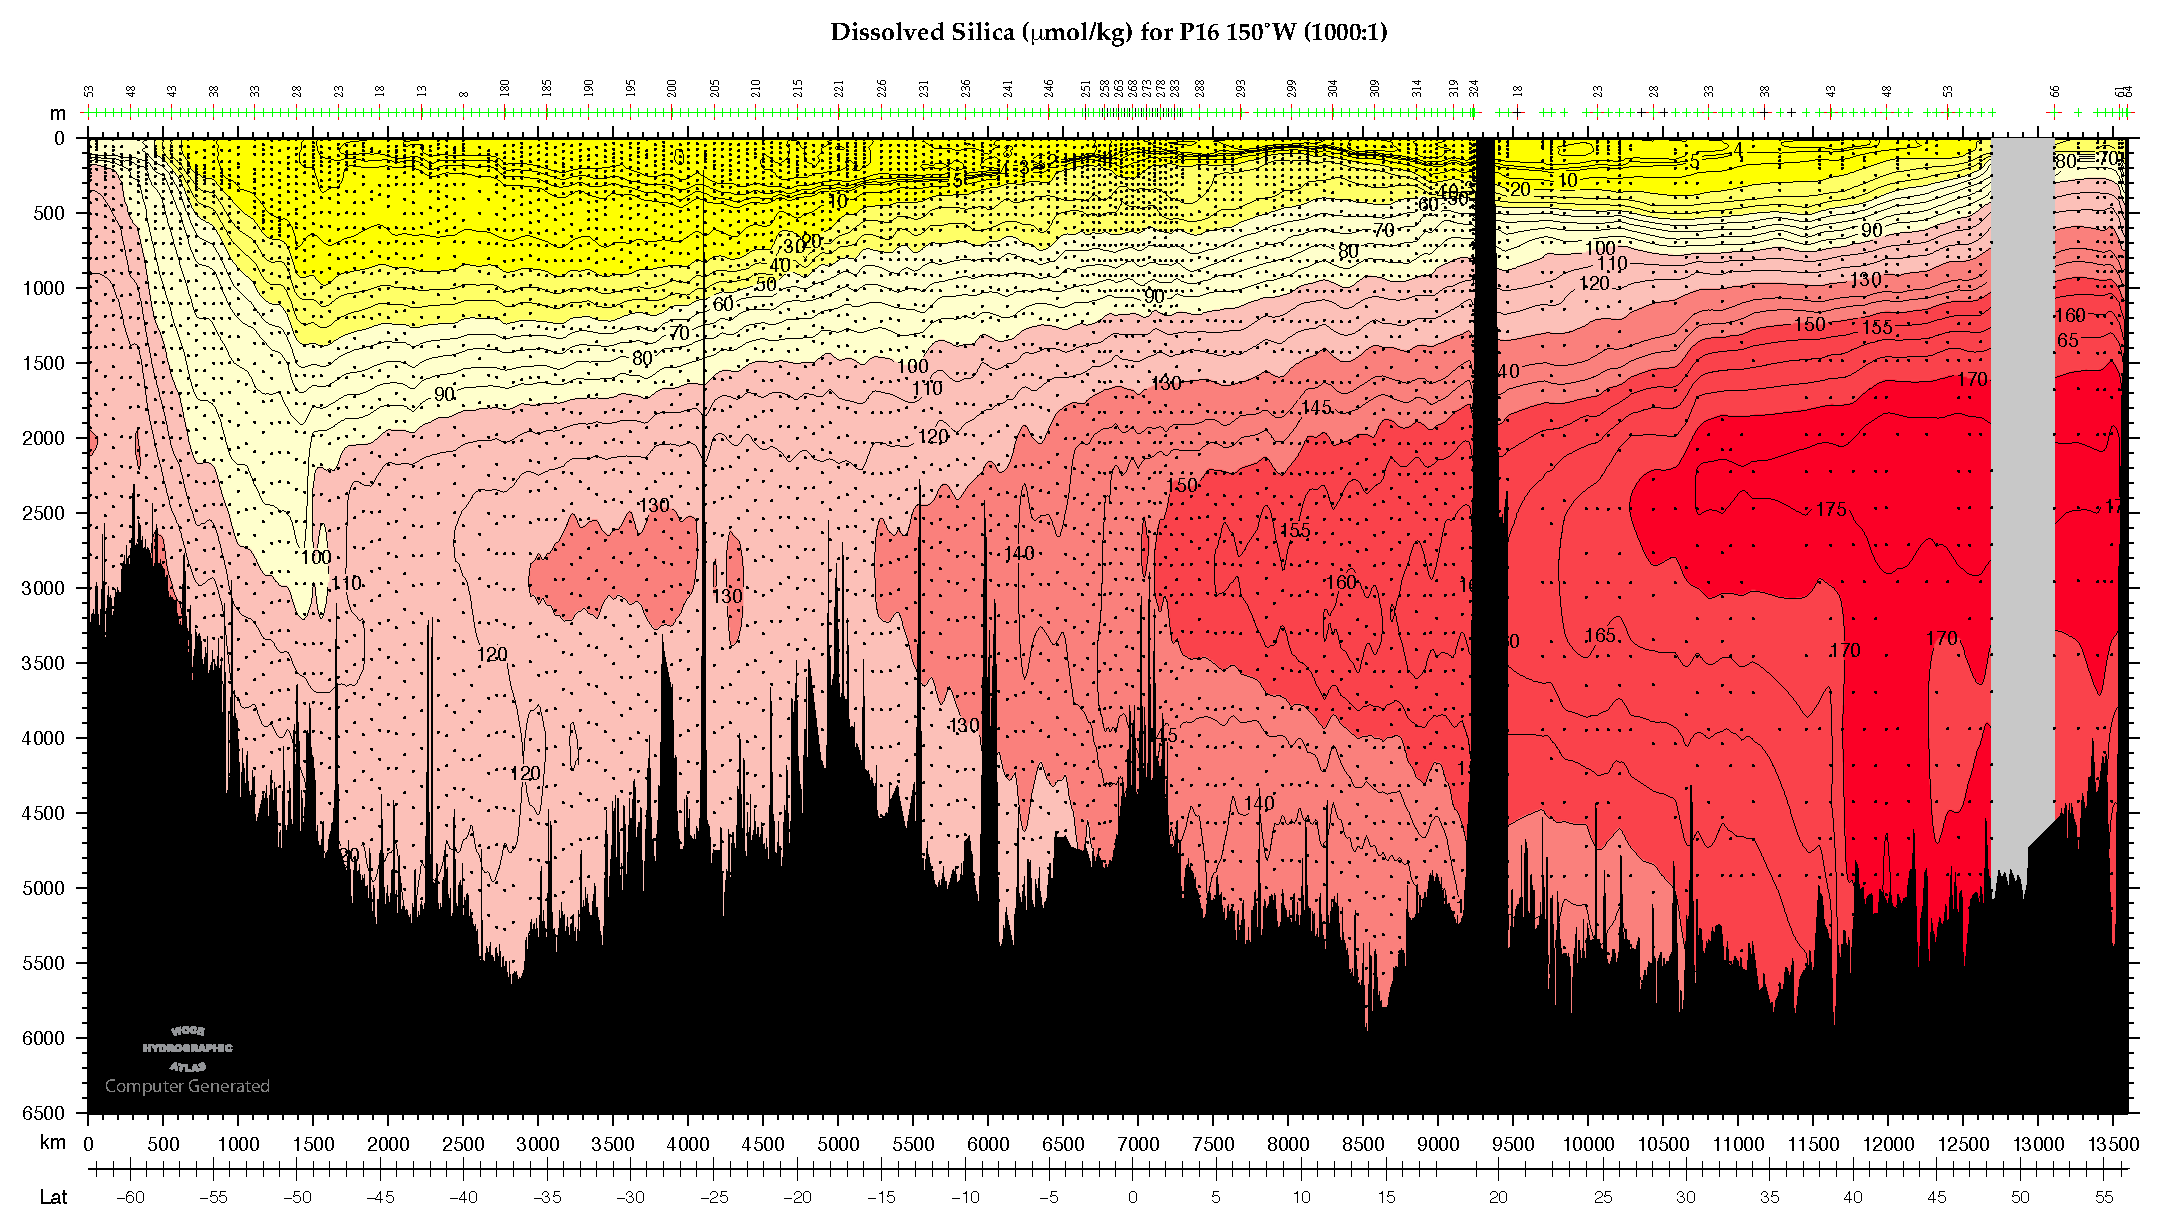
\includegraphics{figs/WaterMasses/P16SilicaCrop}
    \caption{Bio-active tracers in the Pacific ocean along P16.  From the \href{http://whp-atlas.ucsd.edu/pacific_index.html}{WOCE Atlas of the Pacific}. }
    \label{fig:P16BioActive}  
  \end{center}
\end{figure}
\clearpage
\subsection{Radioactive and tracers from the crust}

The age of water can be relatively accurately determined by carbon data using the radioactive isotope $^{14}C$. This carbon isotope is produced in the atmosphere when cosmic rays impact nitrogen molecules.  As such, $^{14}C$ concentrations are highest in the surface ocean (\fref{fig:P16Radioactive}).  $^{14}C$ decays, but unlike bio-active tracers, it decays at a known steady rate, with a half-life of \href{https://en.wikipedia.org/wiki/Carbon-14}{5,730 years}.  Knowing this decay rate, and the relative abundance in the atmosphere, we can arrive at an average age for a water parcel, keeping in mind that there has necessarily been mixing with the water masses above.  From this we can see that the oldest water in the Pacific is probably at about 2500 m depth in the North Pacific. 

There are some caveats to looking at $^{14}C$, tho most obvious one is that the water signal can be contaminated by organic matter raining down from above.  This organic matter will have younger $^{14}C$ in it, so the water will be deduced to be younger than it is.  There is another bias that will make the water look younger, in that if young water is mixed with old water, the age is actually a logarithm of the concentration, and logarithms cannot be added linearly.  This turns out to be a difficult problem, so that accurately estimating the age of the water requires complicated inverses of where the water has been and what water masses have mixed to produce it over its history.  


Recent attempts to estimate water mass age using $^{14}C$ give estimates of water as old as 1500 y in the north Pacific, and at the north end of the Indian Ocean.  Atlantic water tends to be younger, reaching about 700 years old, because it is heavily influenced by the shallower overturning of the North Atlantic Deep Water.  These number speak to the sluggishness of the overturning circulation.  In the Pacific, the bottom water is almost 1000 years old by the time it reaches the equator, or a speed of approximately 7.7 km-per-year in the horizontal, or 
$2.5\times 10^{-7}\ \mathrm{m\,s^{-1}}$ 

\begin{figure}[hbt]
  \begin{center}
    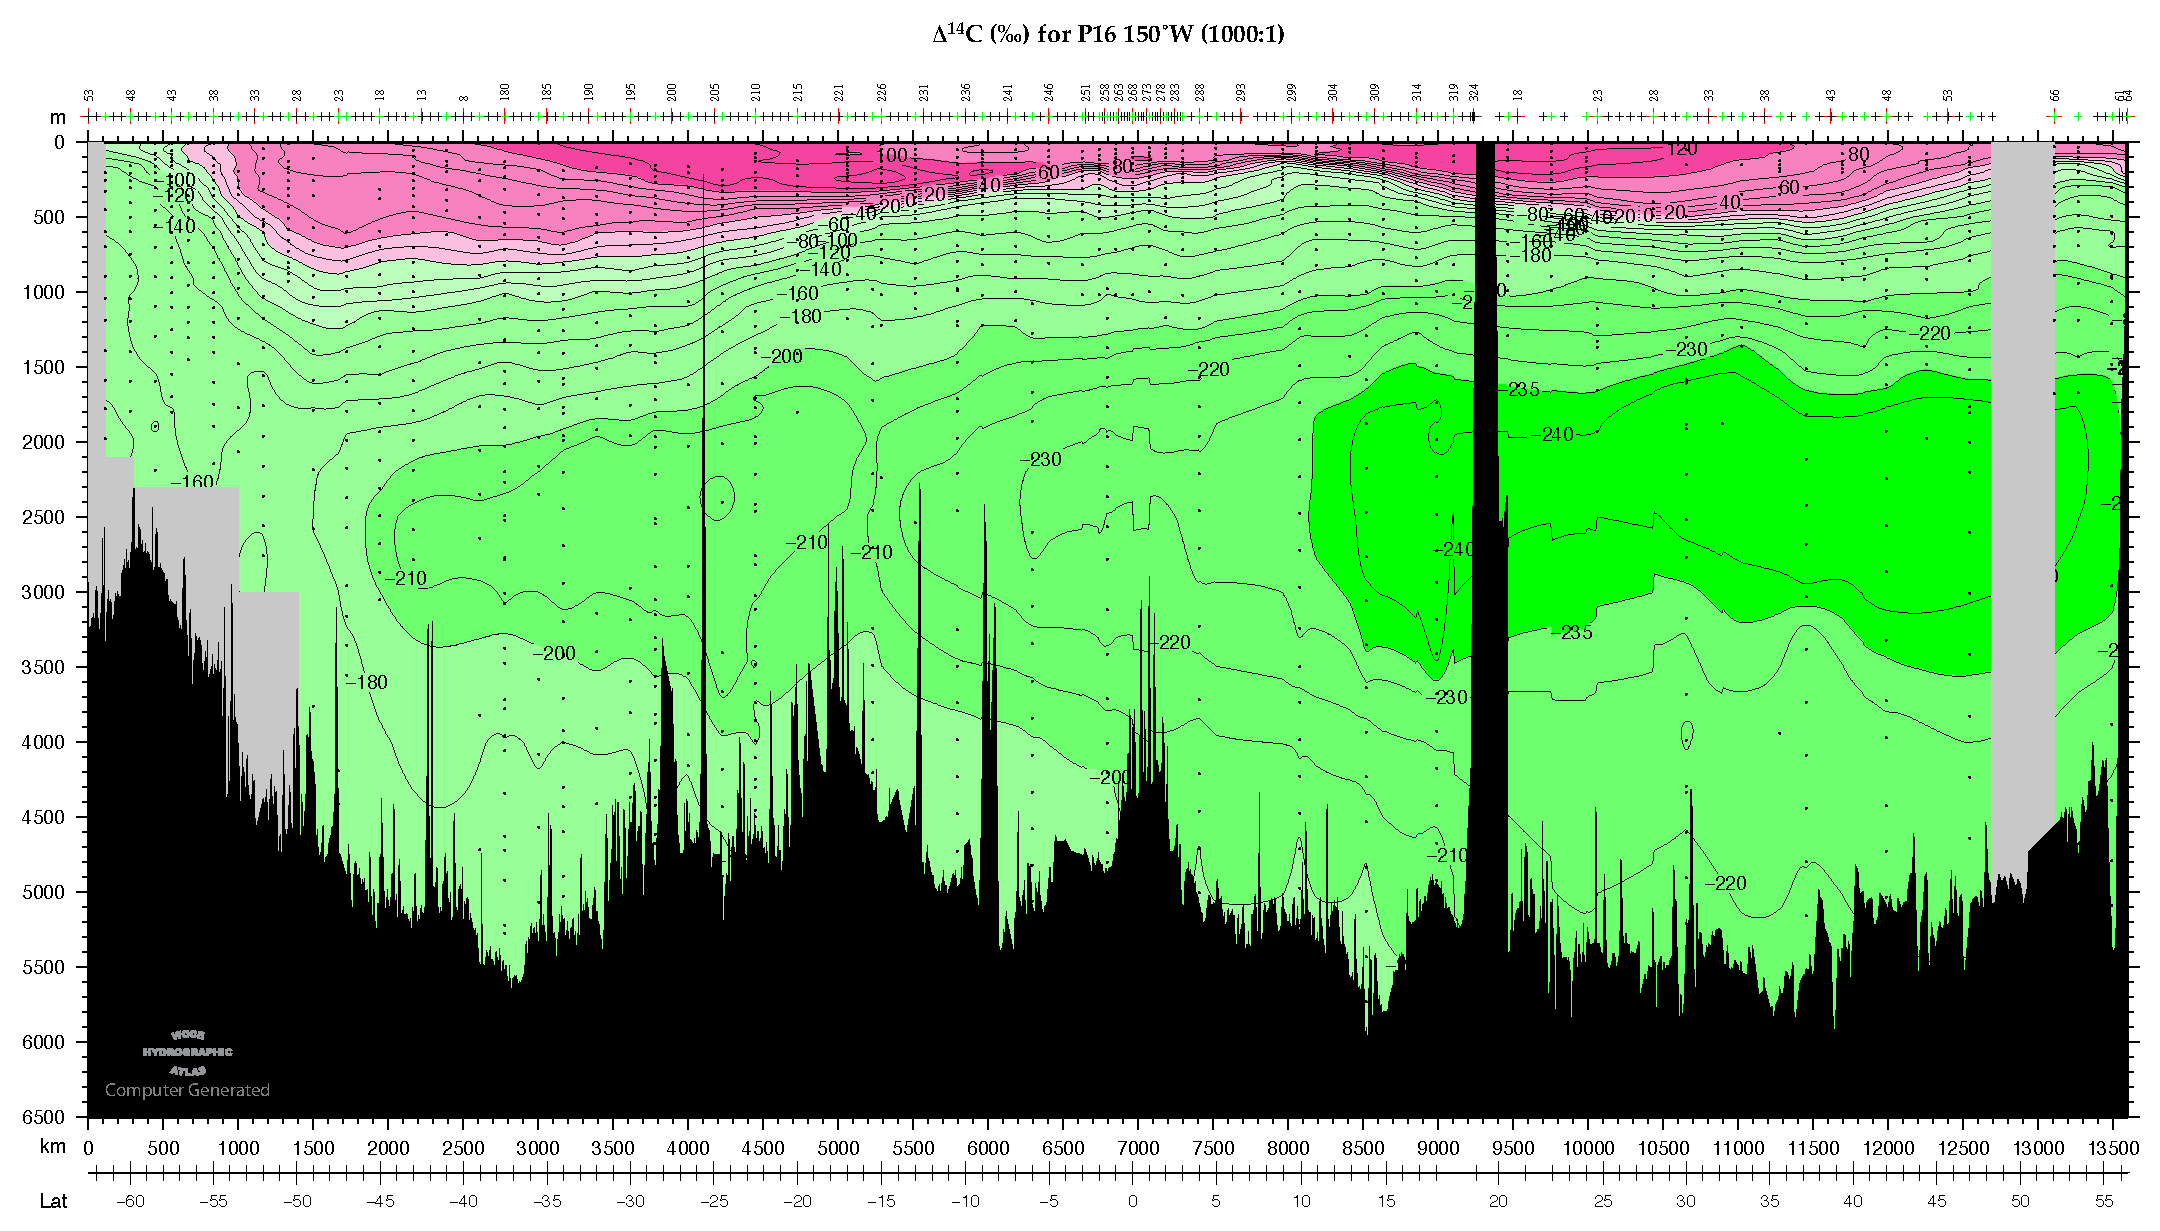
\includegraphics{figs/WaterMasses/P16DC14Crop}
    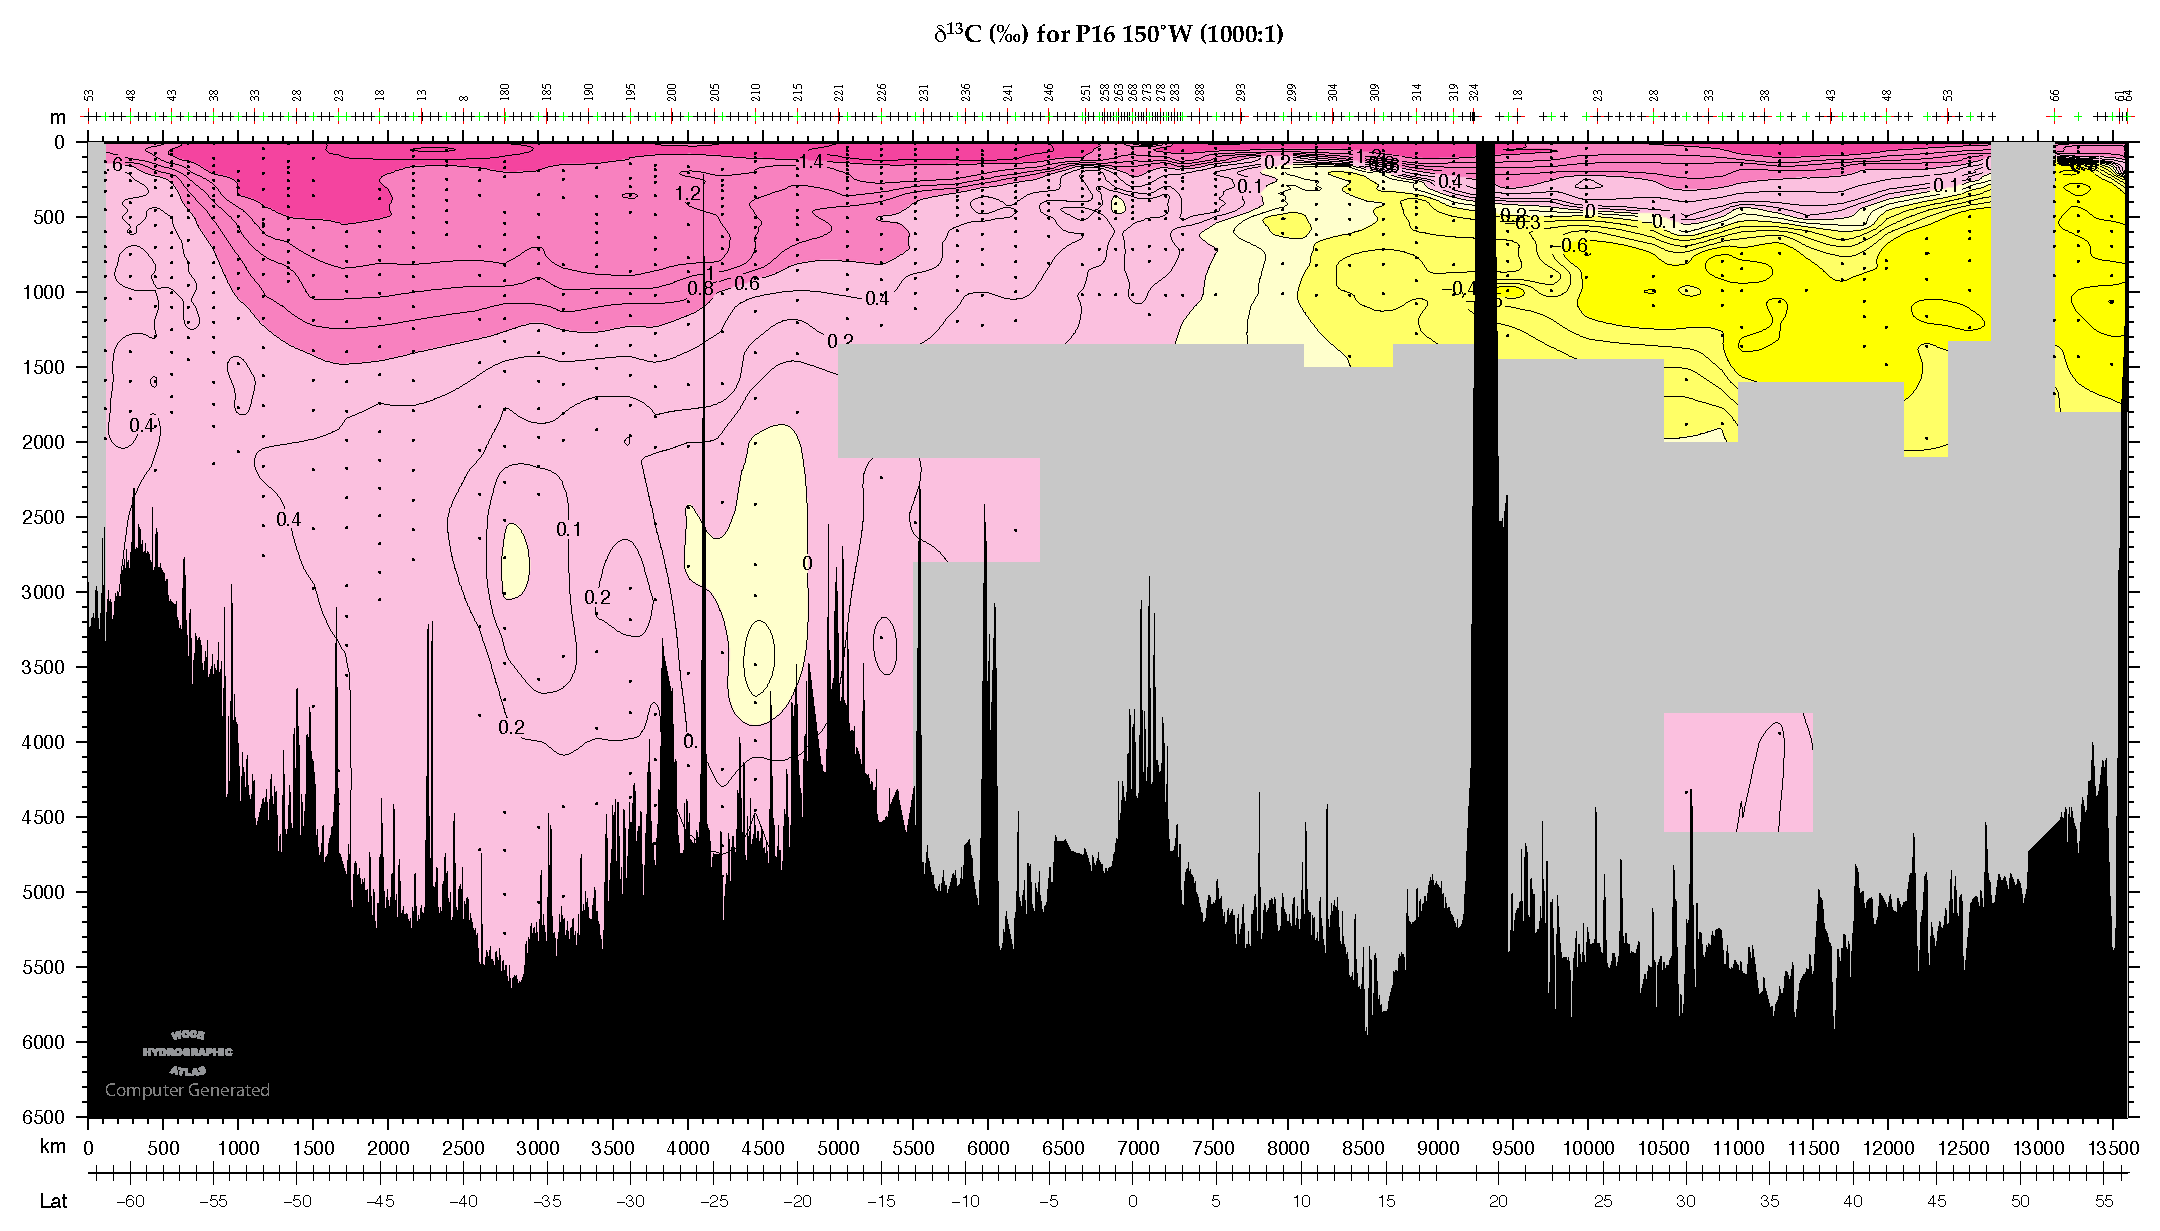
\includegraphics{figs/WaterMasses/P16dC13Crop}
    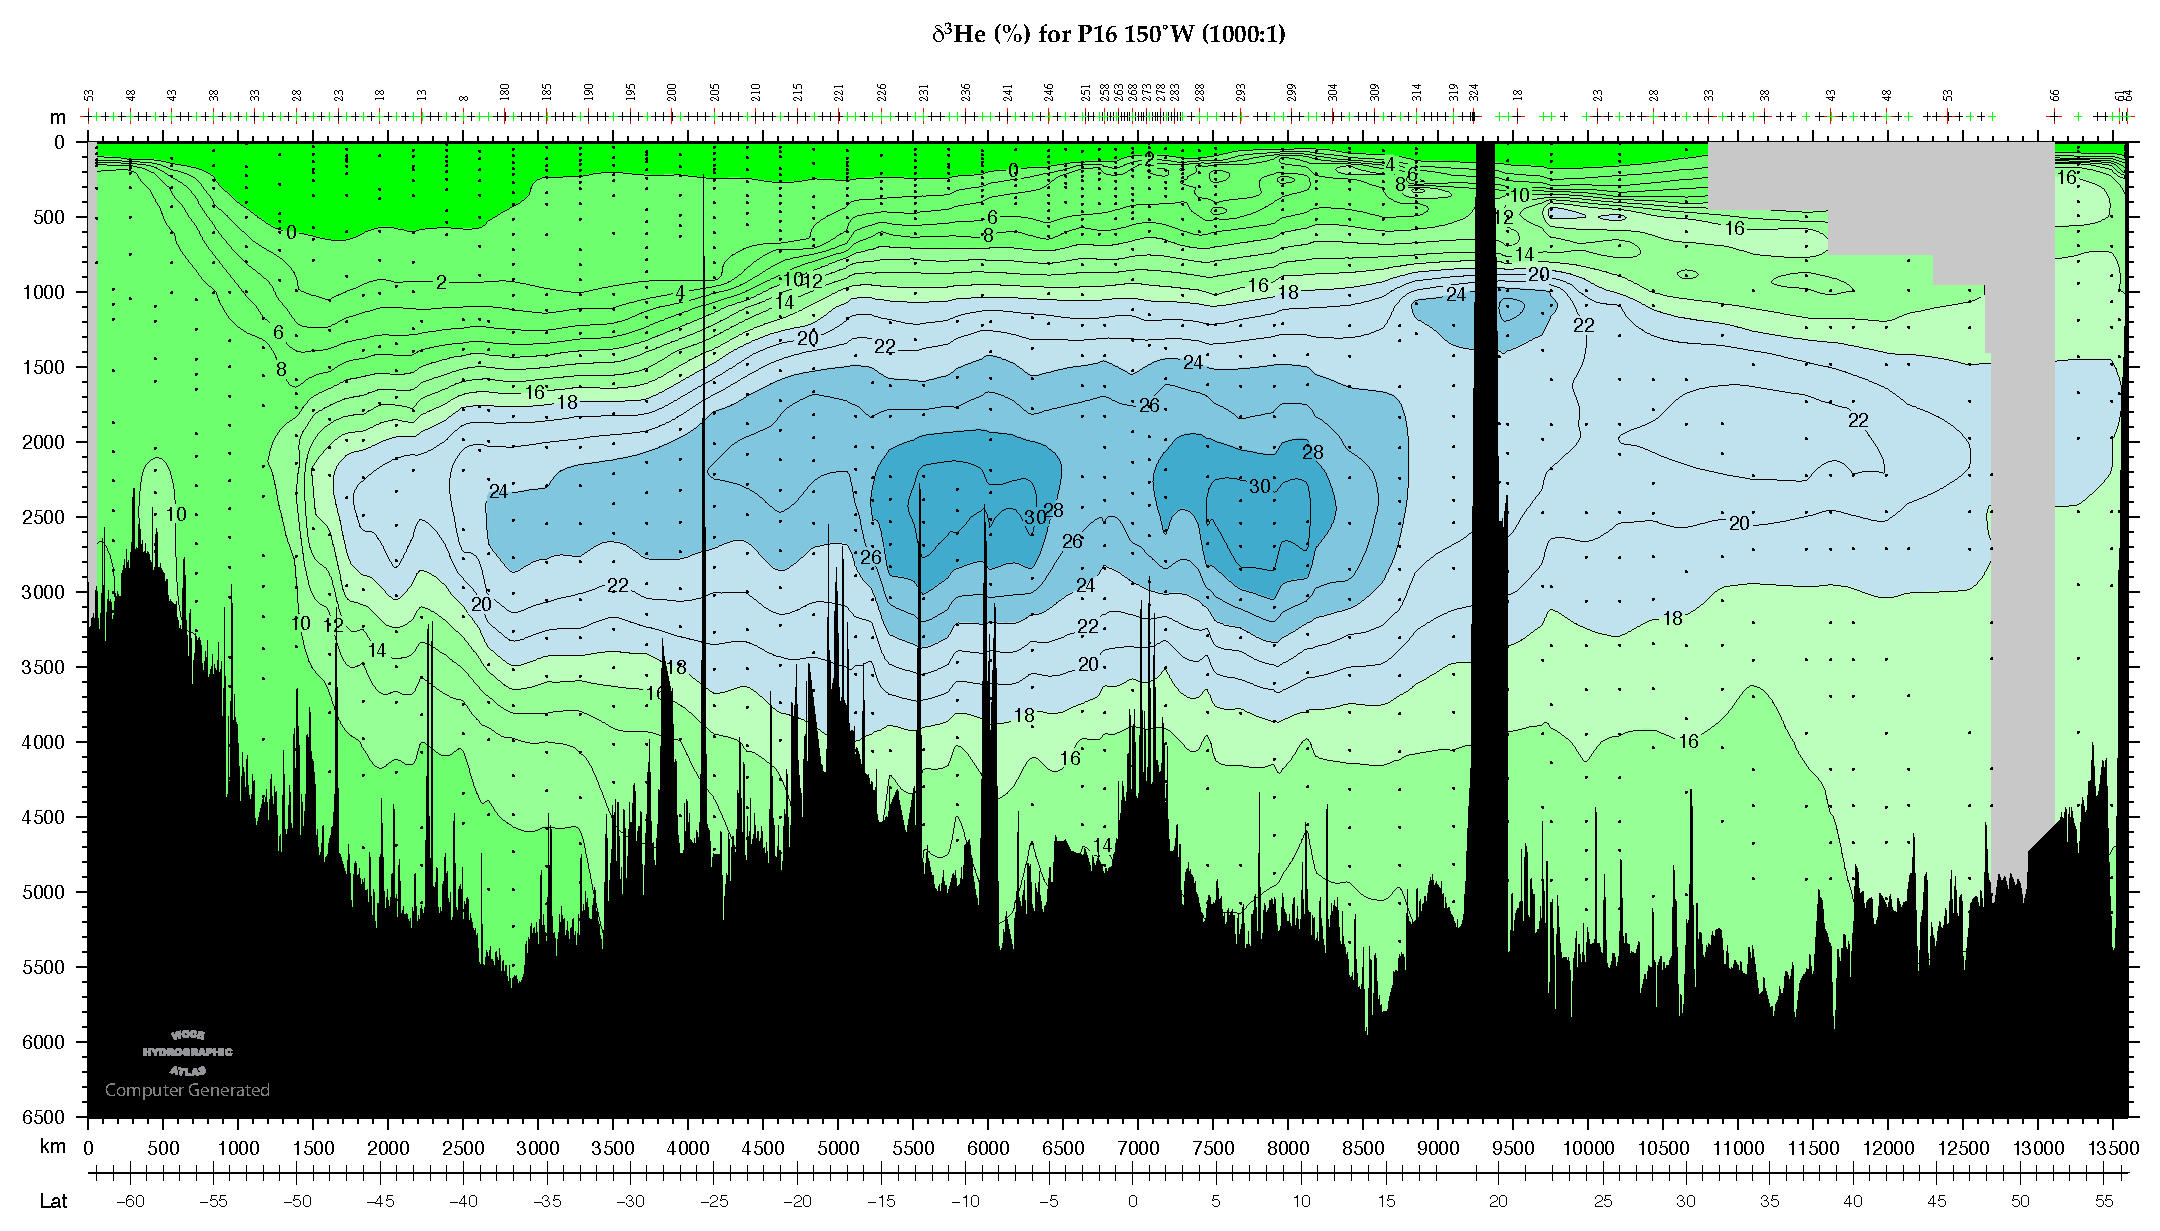
\includegraphics{figs/WaterMasses/P16d3HeCrop}
    \caption{Radioactive and crust tracers in the Pacific ocean along P16.  From the \href{http://whp-atlas.ucsd.edu/pacific_index.html}{WOCE Atlas of the Pacific}. }
    \label{fig:P16Radioactive}  
  \end{center}
\end{figure}

\begin{figure}[hbt]
  \begin{center}
    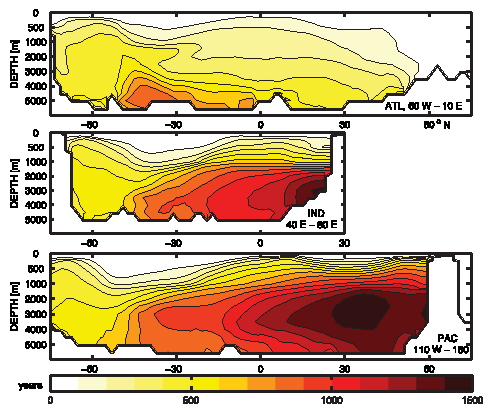
\includegraphics{WaterMasses/GebbieHuybers12Fig8Crop}
    \caption{Average age of water in the three ocean basins as estimated from $^{14}C$ data \citep{gebbiehuybers12}.}
    \label{fig:GebbieHuybers12Fig8}  
  \end{center}
\end{figure}

The isotope $^3He$ is an interesting tracer because it largely comes from ocean hydrothermal vents (\fref{fig:P16Radioactive}c).  The two large peaks in the middle of the section arise because the cruise passed close to the East Pacific Rise at these locations.  


\clearpage
\subsection{Man-made tracers}

Anthropogenic tracers are also useful for tracking ocean processes.  The only problem is that most of these are modern, and hence only track the upper ocean (\fref{fig:P16Manmade}).  In fact these tracers give an idea of just how \emph{slow} the circulation is.  Tritium is largely a product of nuclear weapons testing, which was predominantly carried out in the atmosphere in the 1960s (\fref{fig:TritiumOttawa}).  This makes for a nice tracer spike that shows how far water transited in the 35 years when  the WOCE lines were run (\fref{fig:P16Manmade}).  Similarly, CFC-11 and -12 saw an exponential increase in emissions until the 1970s when the danger of CFCs to the ozone layer was realized, and dropped off after the Montreal Protocol, when they were finally banned.  

\begin{figure}[hbt]
  \begin{center}
    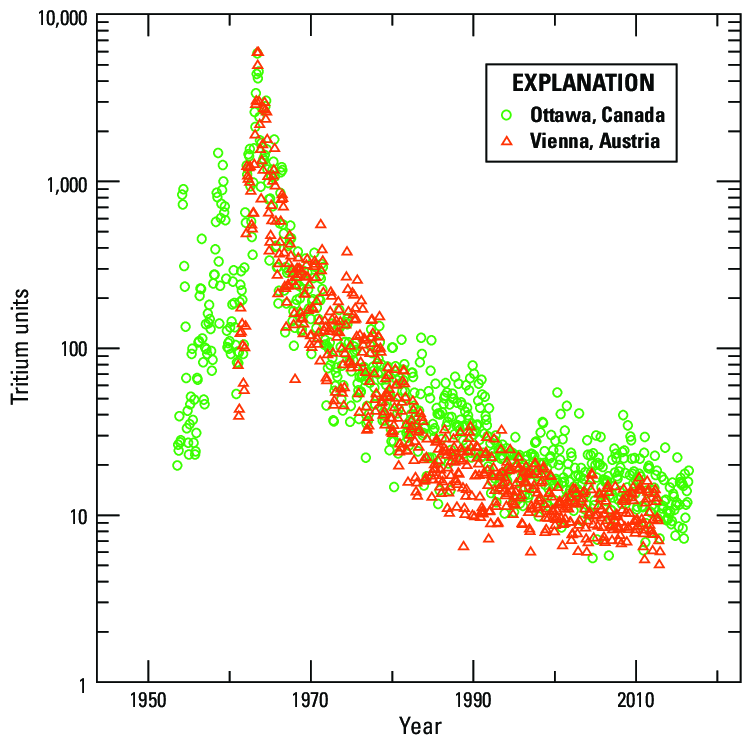
\includegraphics[width=3in]{figs/WaterMasses/TritiumOttawa}
    \caption{Tritium time series in the atmosphere measured at Ottawa and Vienna.  Note the logarithmic vertical scale, so almost all the input was in the 1960s}
    \label{fig:TritiumOttawa}  
  \end{center}
\end{figure}

\begin{figure}[hbt]
  \begin{center}
    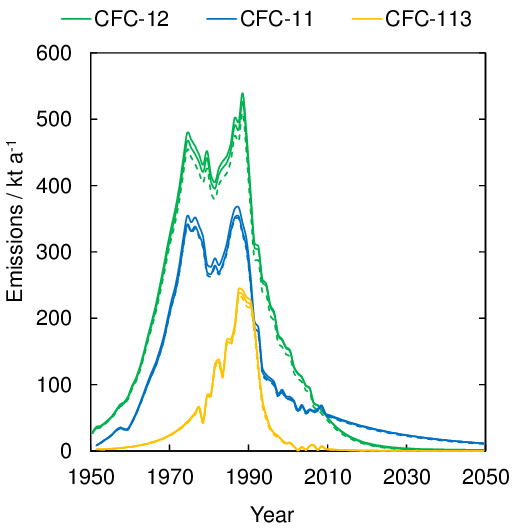
\includegraphics[width=3in]{figs/WaterMasses/Emissions-estimates-for-CFC-11-blue-CFC-12-green-and-CFC-113-orange-based-on.png}
    \caption{Global CFC emissions, estimated from atmospheric concentrations \citep{Allin_2015}.}
    \label{fig:CFCEmmisions}  
  \end{center}
\end{figure}

All three man-made tracers had relatively minimal penetration into the  deep ocean when the P16 lines were occupied, but \emph{clearly} show up in the Southern Ocean as a plume of high concentrations.  Of course the upper ocean has substantial quantities of these tracers.  

\begin{figure}[hbt]
  \begin{center}
    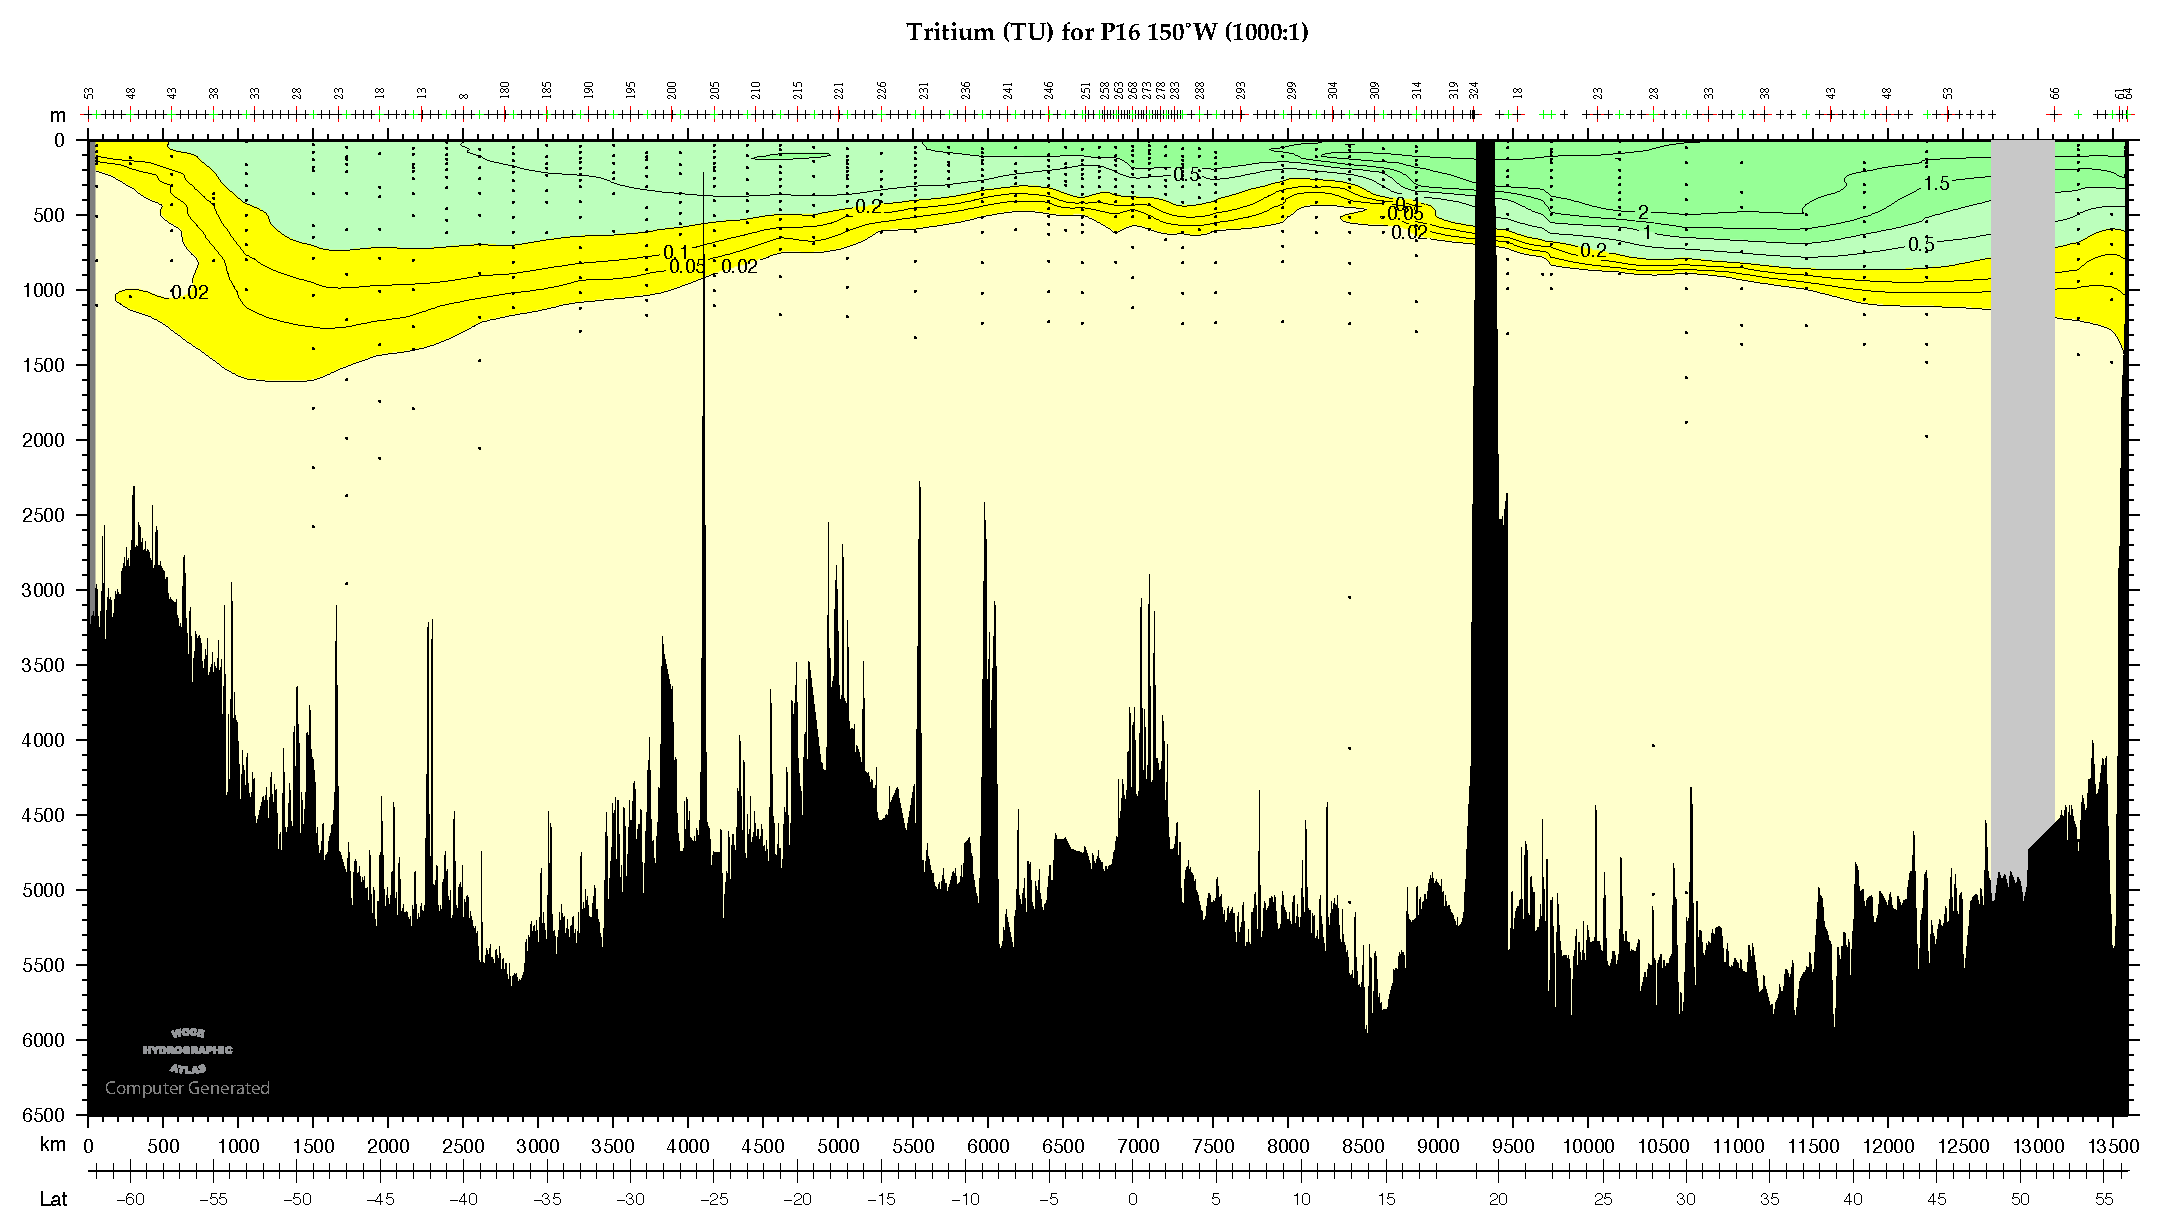
\includegraphics[width=3.8in]{figs/WaterMasses/P16TritiumCrop}
    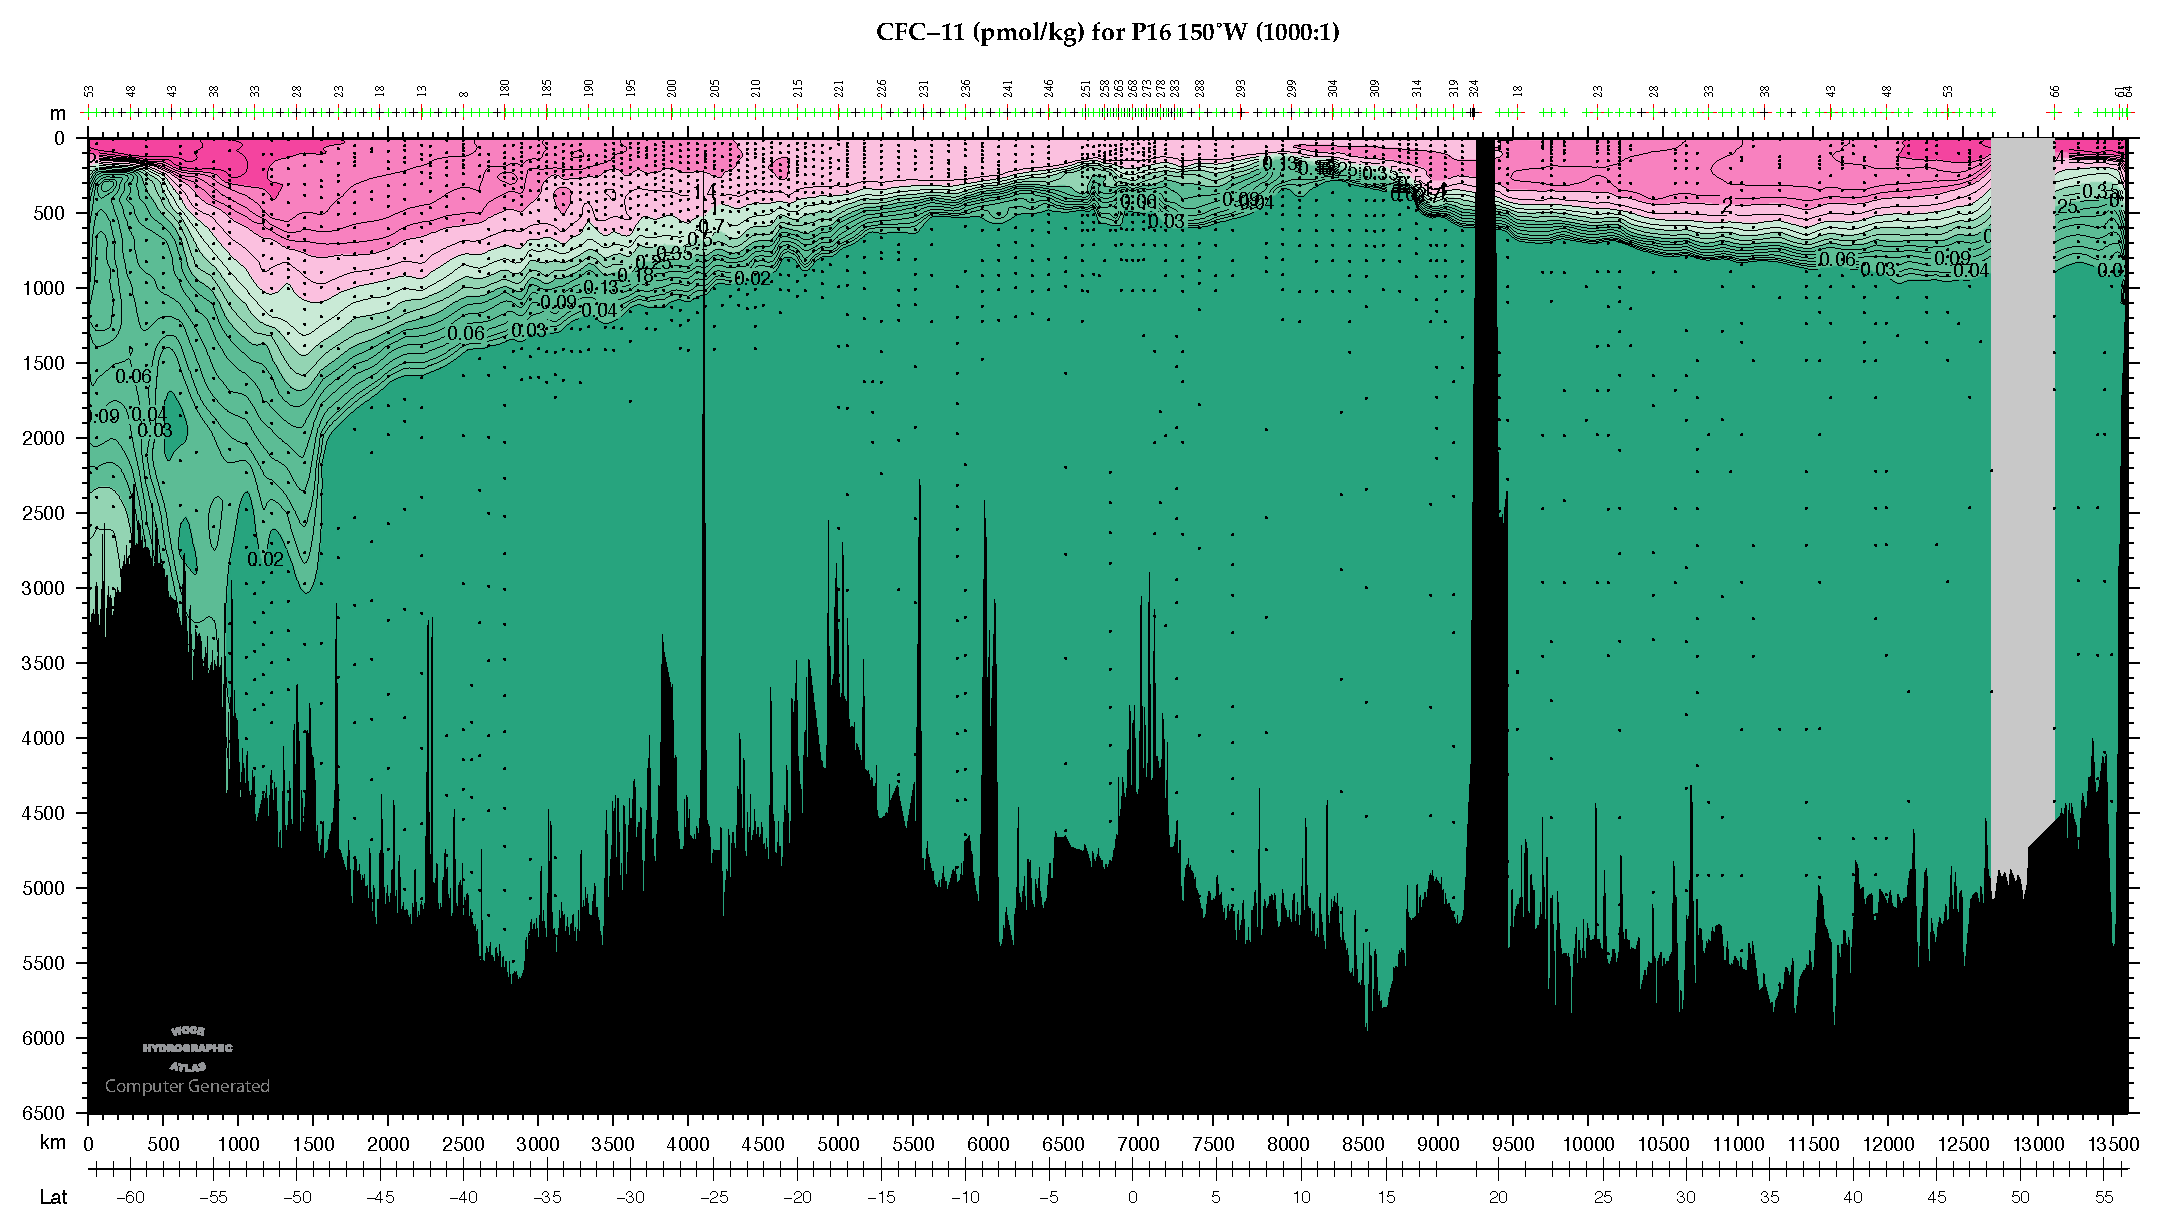
\includegraphics[width=3.8in]{figs/WaterMasses/P16CFC11Crop}
    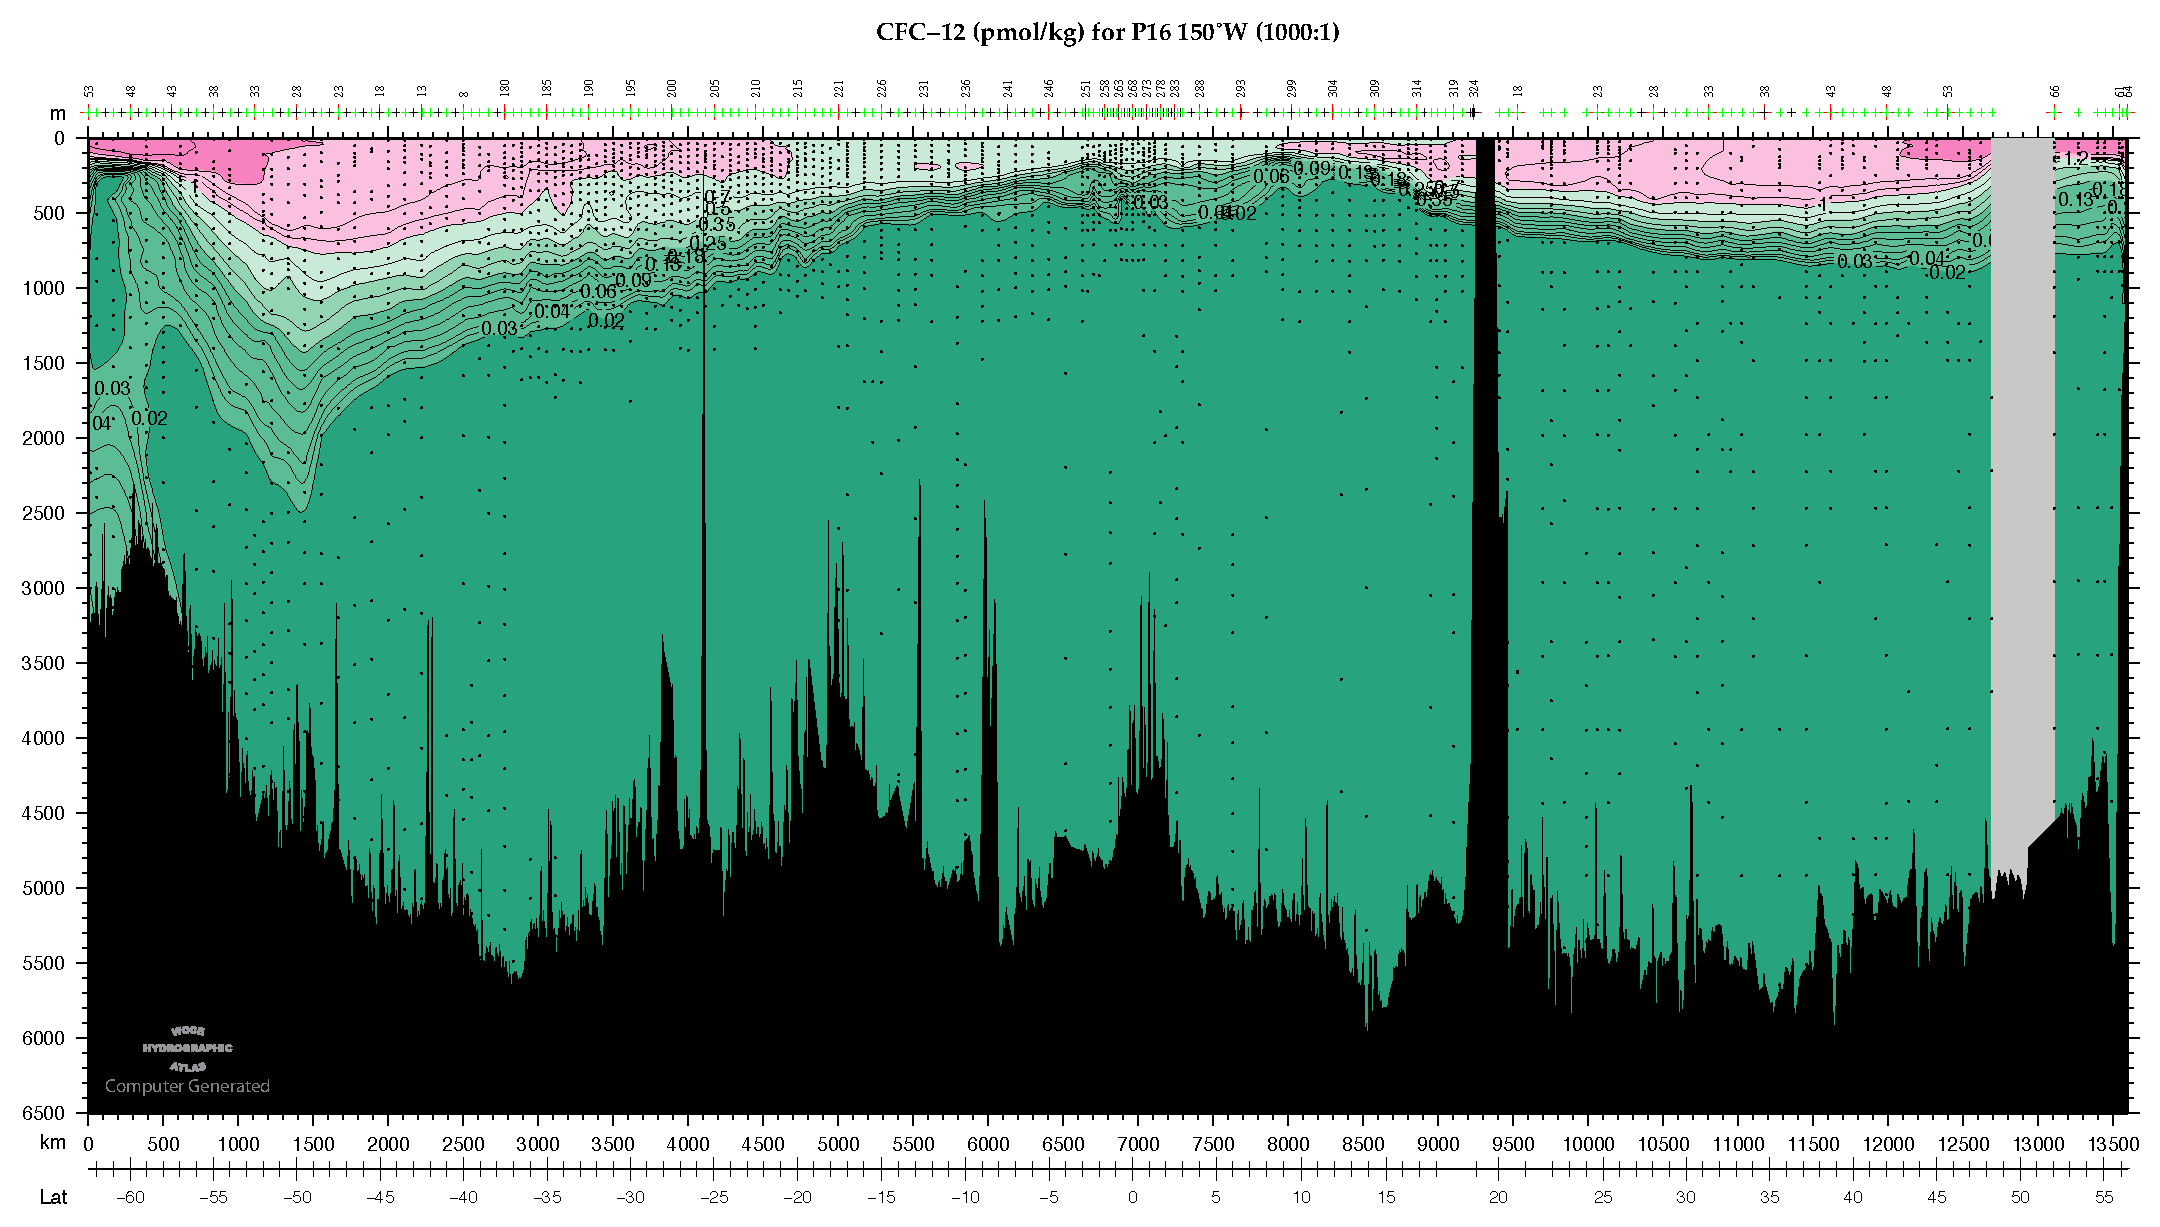
\includegraphics[width=3.8in]{figs/WaterMasses/P16CFC12Crop}
    \caption{Man-made tracers along P16.  From the \href{http://whp-atlas.ucsd.edu/pacific_index.html}{WOCE Atlas of the Pacific}. Note that this section was collected in 1991.}
    \label{fig:P16Manmade}  
  \end{center}
\end{figure}

The WOCE cruises along P16 spanned the years 1991-1993.  These waters were resampled again as part of the CLIVAR/GO-SHIP program in 2014-2015 (\fref{fig:P16CFCWOCECLIVAR}) and the intervening 21-24 years do show some change.  These changes are particularly pronounced in the intermediate waters with CFCs transiting substantially deeper and more equatorward.  The CFCs also appear to have mixed from the surface ocean to deeper, with the CFC-gradient descending around 200 m in most of the basin. In the deep ocean, however, there is still little evidence of CFC penetration.  Looking south of 60 S, there is some evidence that high CFC waters are trying to push over the ridge, and there are perhaps some heightened values along the bottom south of 30 S, but if so, then these values are very diluted.  Overall the manmade tracers show how old and slow the deep ocean bottom circulation is.  

\begin{figure}[hbt]
  \begin{center}
    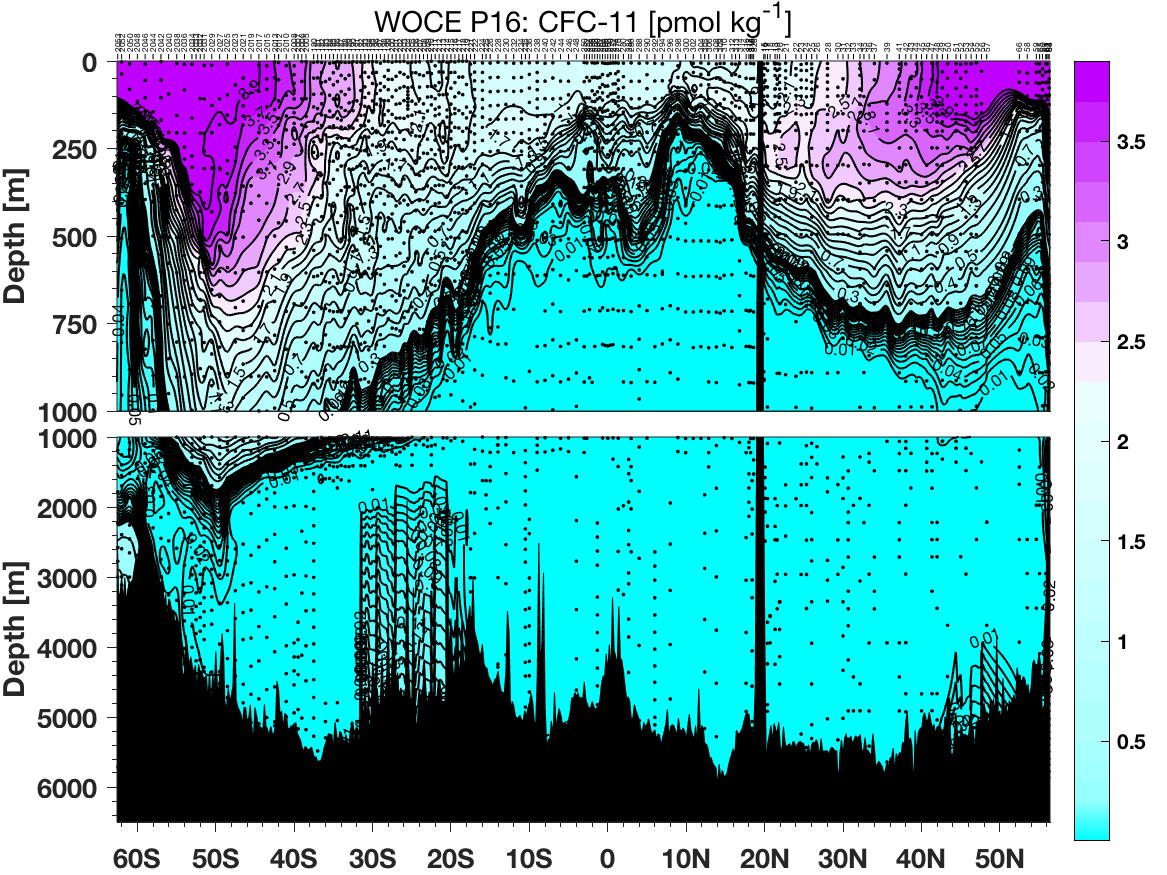
\includegraphics[width=3.8in]{figs/WaterMasses/p16_cfc11_woce.png}
    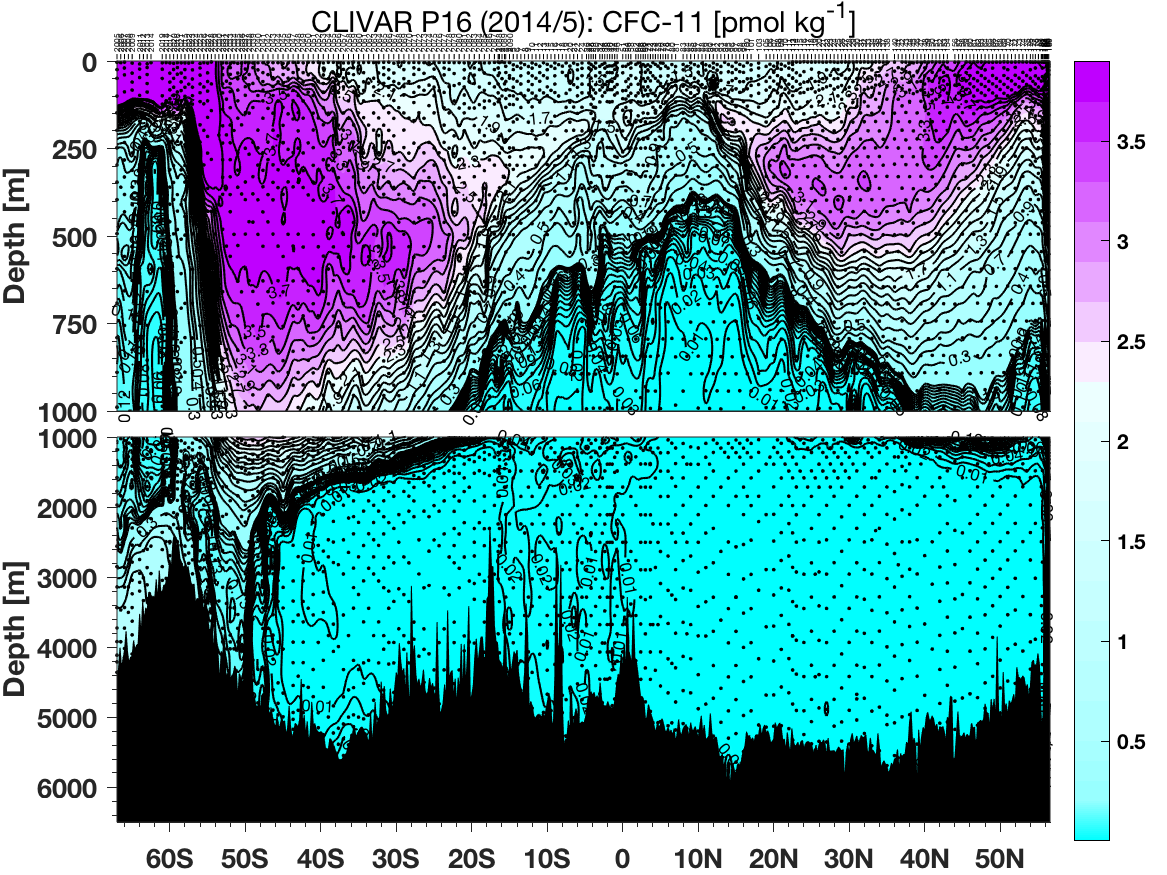
\includegraphics[width=3.8in]{figs/WaterMasses/p16_cfc11_2014_2015.png}
    \caption{CFC-11 along P16, during WOCE (1991-93) and the GO-SHIP/CLIVAR re-occupation (2015-16).  Note there are some poor-quality samples in the WOCE section deeper than 2000 m between 30S and 15 S.  Figure courtesy S. Mecking.}
    \label{fig:P16CFCWOCECLIVAR}  
  \end{center}
\end{figure}


\clearpage

\section{Deep water formation processes}

The densest water in the global ocean is formed at the high latitudes.  The densest water is formed in the Wedell and Ross Seas in the southern ocean.  Deep water formation processes are notoriously hard to observe, but the mechanisms are relatively well understood.  

\subsection{Antarctic Bottom Water}

\begin{marginfigure}
  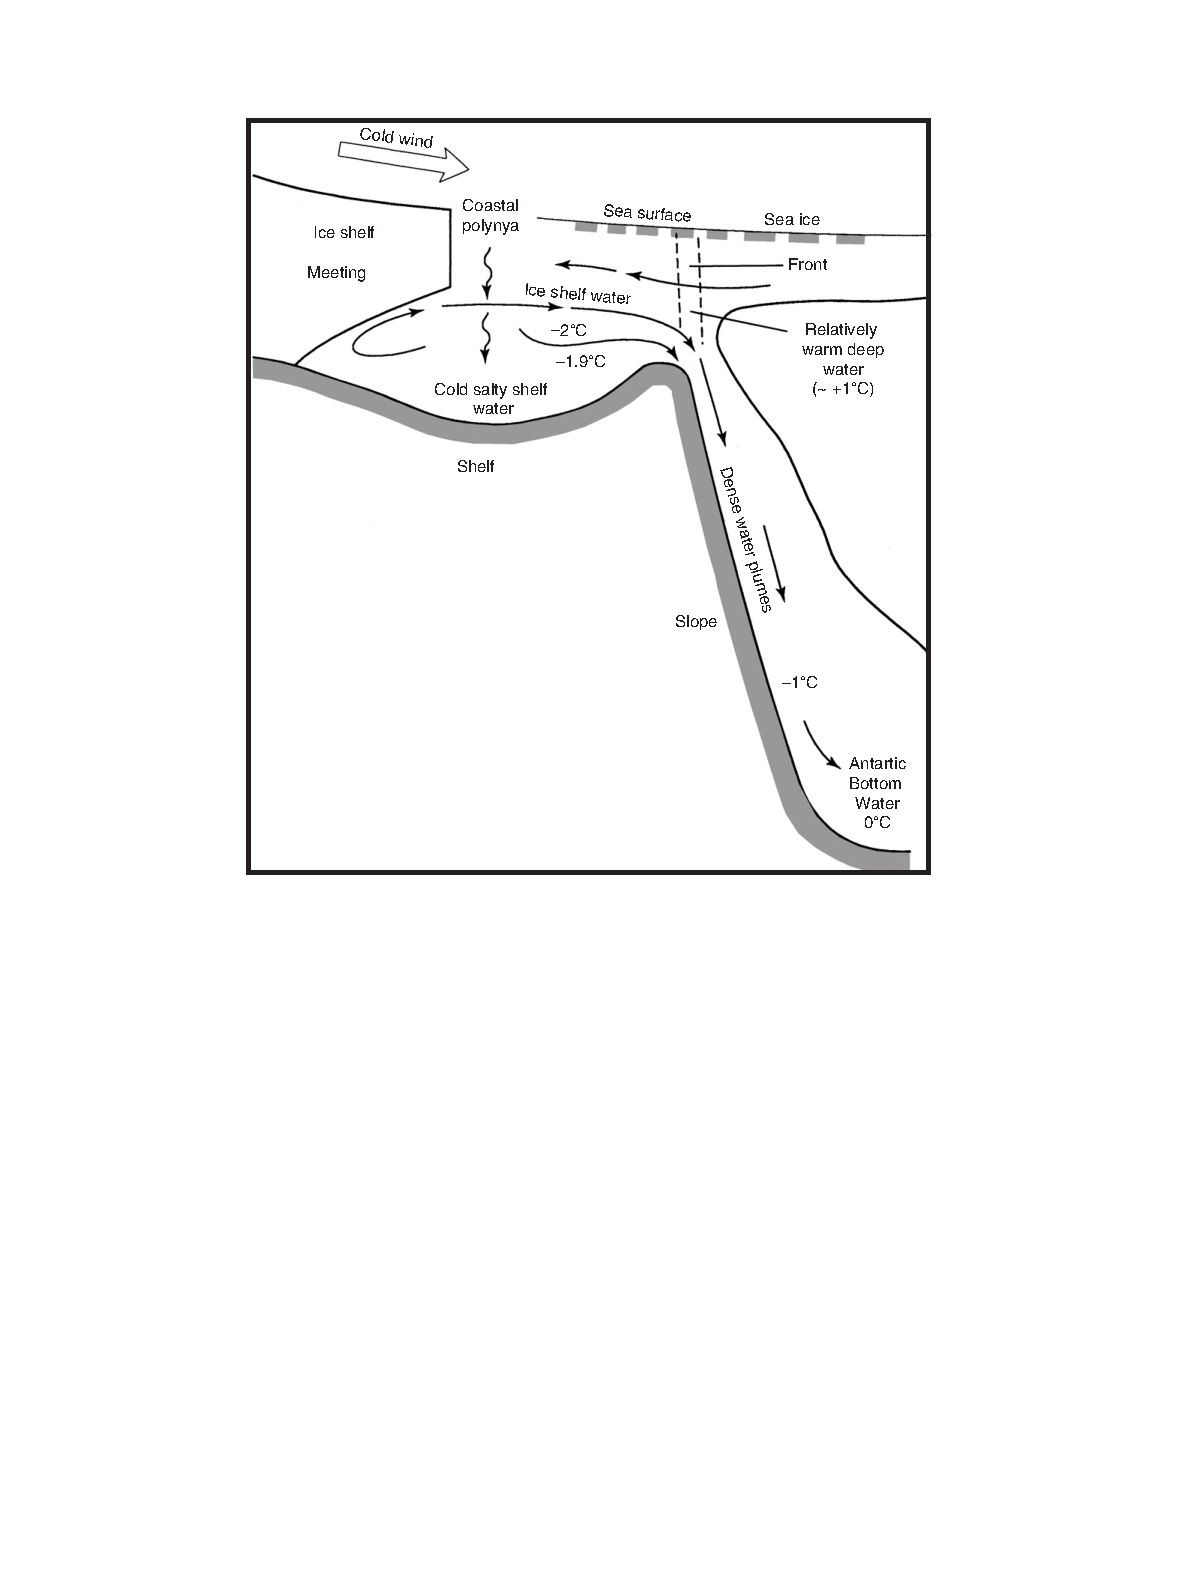
\includegraphics[width=2.3in]{figs/WaterMasses/Gordon09Fig3}
    \caption{Schematic of deep water formation in the marginal seas of Antarctica \citep{gordon01}.}
    \label{fig:Gordon09Fig3}  
\end{marginfigure}

In the Antarctic, dry cold continental air blows off the continent \fref{fig:Gordon09Fig3}.  These winds can be quite strong and work to push sea ice off the landmass, often opening up \emph{leads} and \emph{polynyas}, despite the cold air.  These polynyas are regions of very large heat loss, both latent and sensible.  Further, they create more ice (which is then pushed offshore), and ice creation leads to brine rejection, which makes the water very salty.  

Detailed observations in the Southern ocean make this process clear \fref{fig:stewartthompson16}.  In these observations, the cold water that comes from the shallower basins to the southeast are observed hugging continental slope.  The very cold water at the bottom is colder than Antarctic Bottom Water, but mixes with the shallower as it descends the slope to make water that is between -1 and 0 C.  

\begin{figure}[hbt]
  \begin{center}
  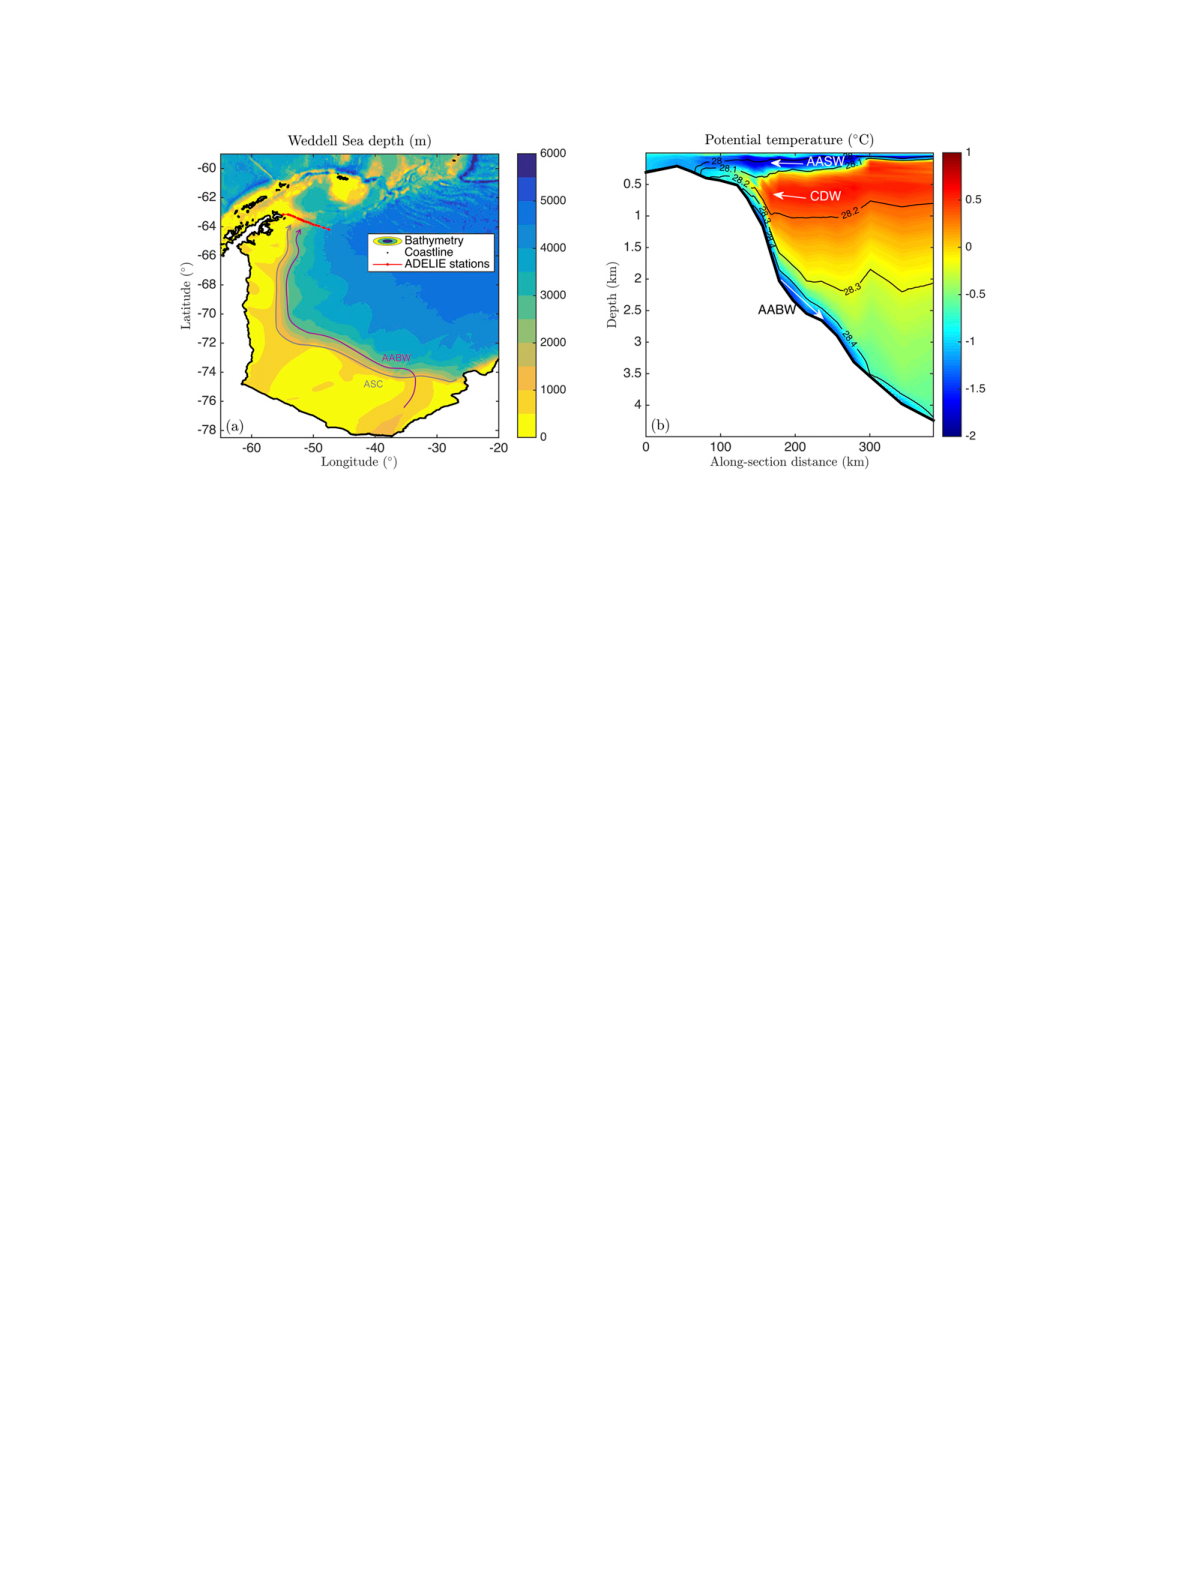
\includegraphics{figs/WaterMasses/StewartThompson16Fig1}
    \caption{bathymetry of the Wedell Sea, and a section of density  contours with temperature coloured underneath.  Note the cold dense water sinking along the continental slope. \citep{stewartthompson16}.}
    \label{fig:stewartthompson16}  
  \end{center}
\end{figure}



\subsection{North Atlantic Deep Water}

North Atlantic Deep Water starts in a similar way to Antarctic Bottom Water, with an origin on the Barents Sea shelf.  Conversely to the Antarctic, this water forms largely free from ice cover, and hence brine rejection is not too important a part of the process.  This cold water flows into the Greenland Sea where it mixes with cold water experiencing convection (\fref{fig:NADWSketch}).  This water pours over the Denmark Straits just east of Greenland, and is further diluted with warm salty water from the North Atlantic.  This current is added to from convection in the Larbador Sea.  

\begin{figure}[hbt]
  \begin{center}
    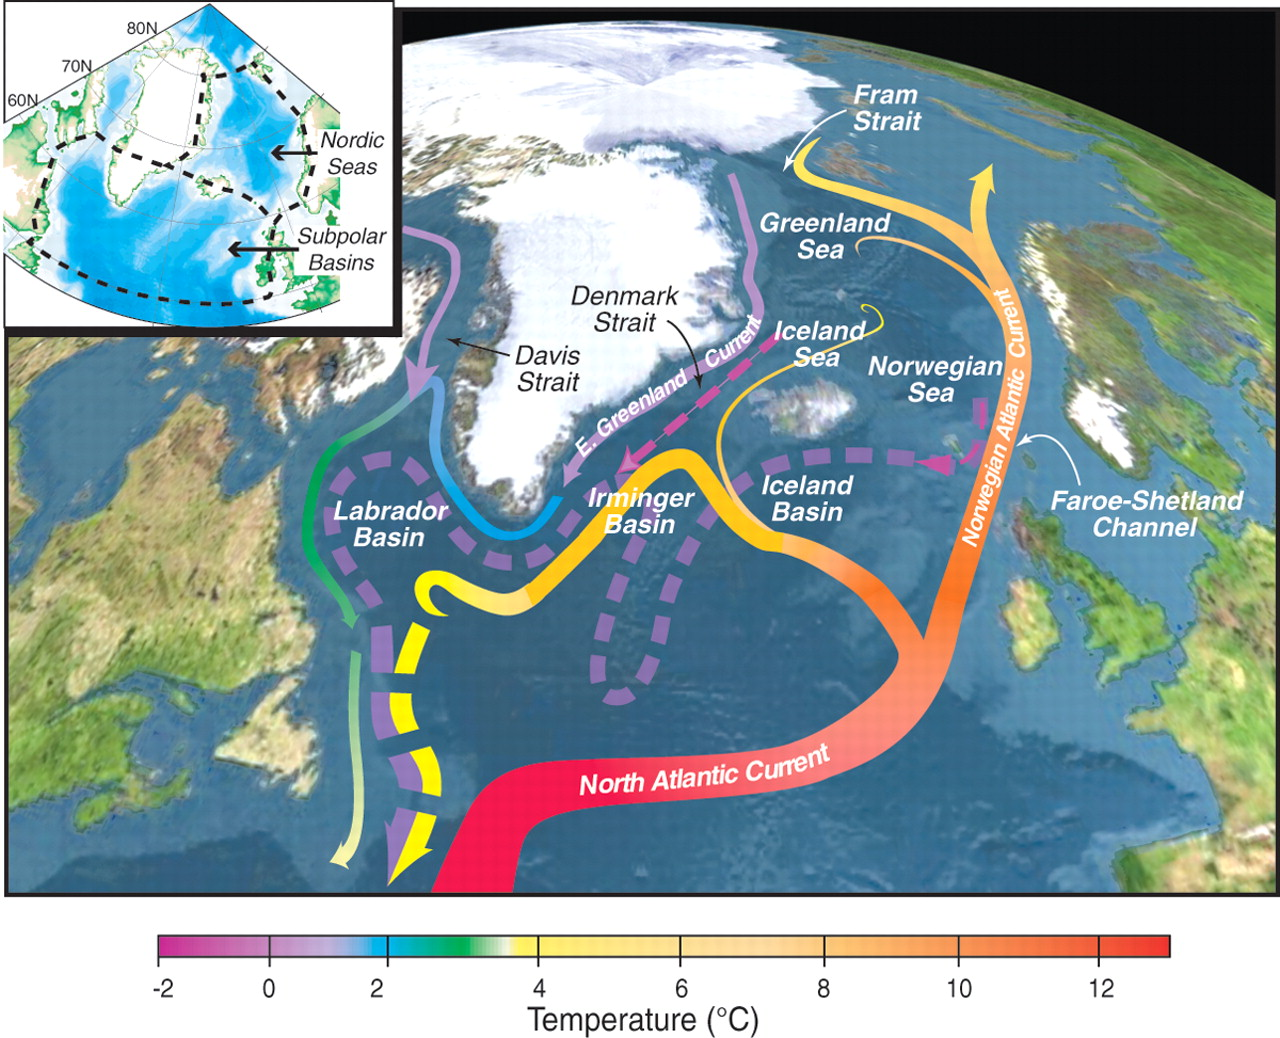
\includegraphics{figs/WaterMasses/NADWSketch}
    \caption{Sketch of paths taken by North Atlantic Deep Water. \citep{currymauritzen2005} }
    \label{fig:NADWSketch}  
  \end{center}
\end{figure}

Deep-water convection is very easy to observe in the Labrador Sea, between Labrador and Greenland.  In the winter, convective mixing can create a mixed layer that is over 2000 m deep \fref{fig:Lazier01Fig9}.  This is caused by cooling, and mixing of relatively fresh water near the surface with warmer saltier water that comes in from the side.  This process varies each year, and sometimes the convection is not as deep in one year as in other years (\fref{fig:KiekeYashayaev15}).  In some years there is no convection at all, like 2007, whereas in others there is very deep convection, like in 2008.   

\begin{figure}[hbt]
  \begin{center}
    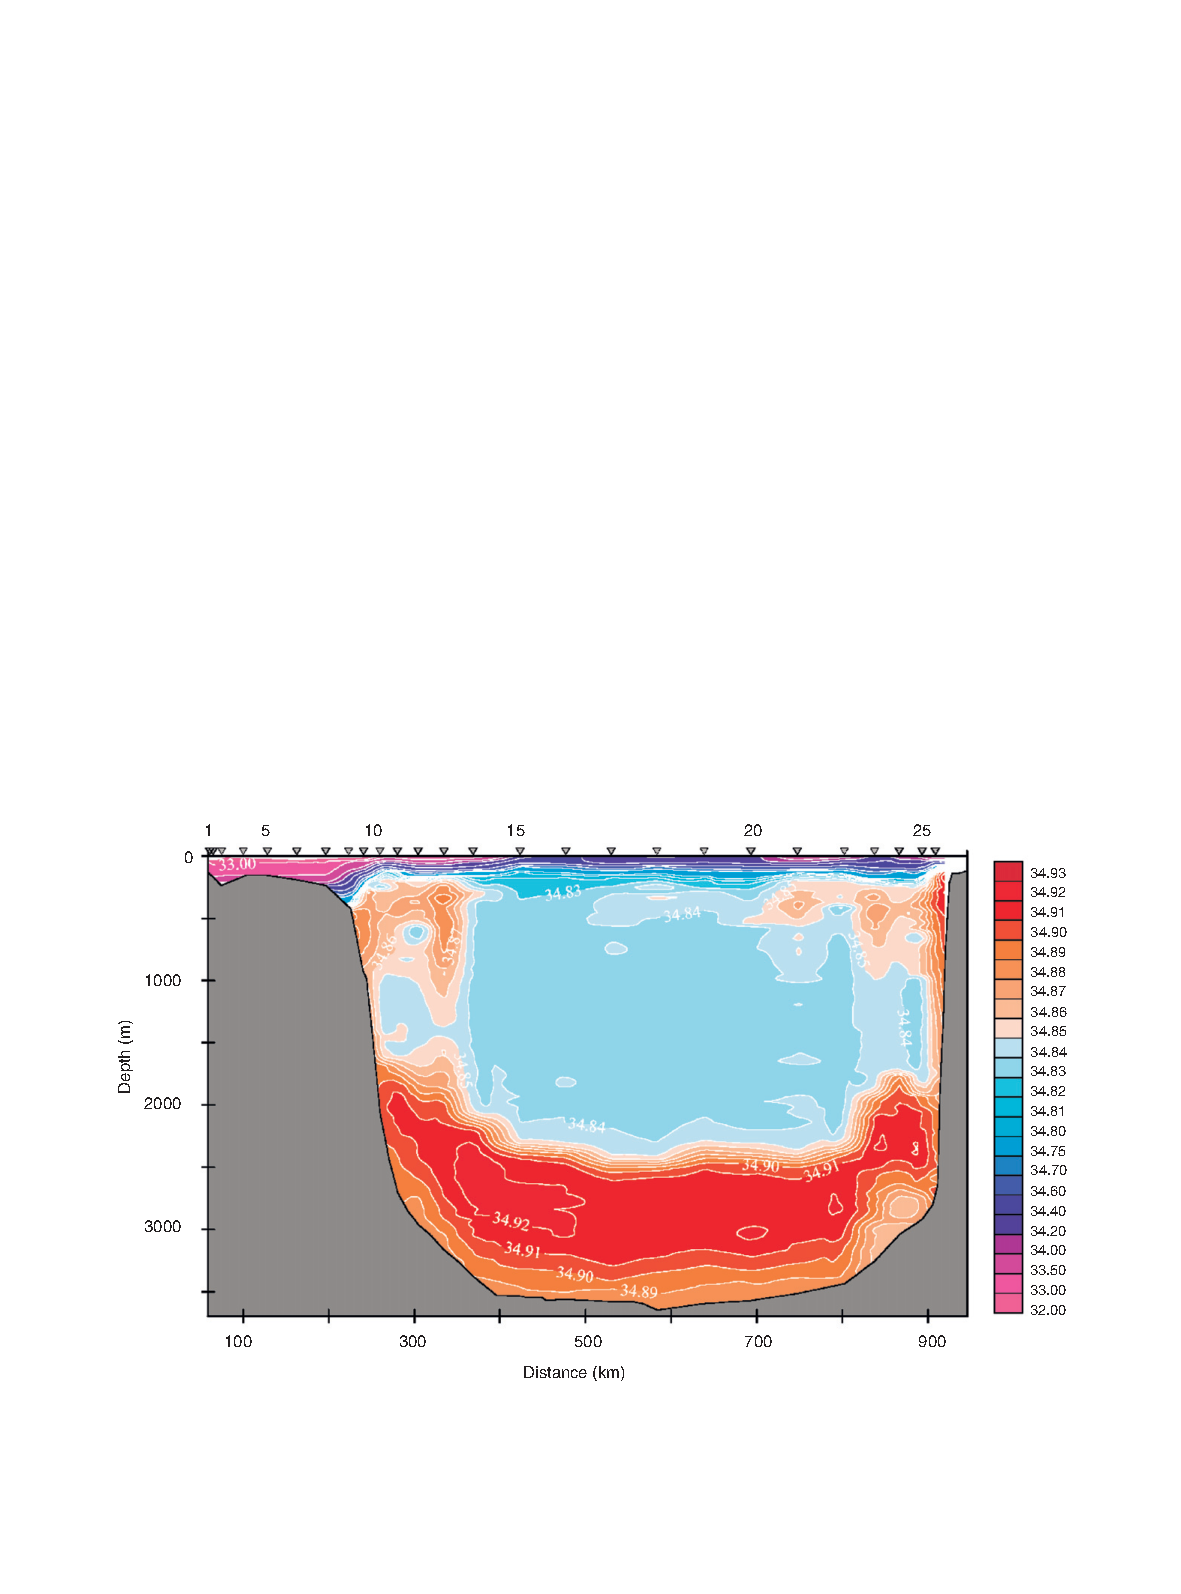
\includegraphics{figs/WaterMasses/Lazier01Fig9}
    \caption{Evidence of convection in the Labrador Sea from a section across the Sea in June 1993.  Note the very homogeneous water in the central Labrador Sea, with mixing deeper than 2000 m.  }
    \label{fig:Lazier01Fig9}  
  \end{center}
\end{figure}


\begin{figure}[hbt]
  \begin{center}
    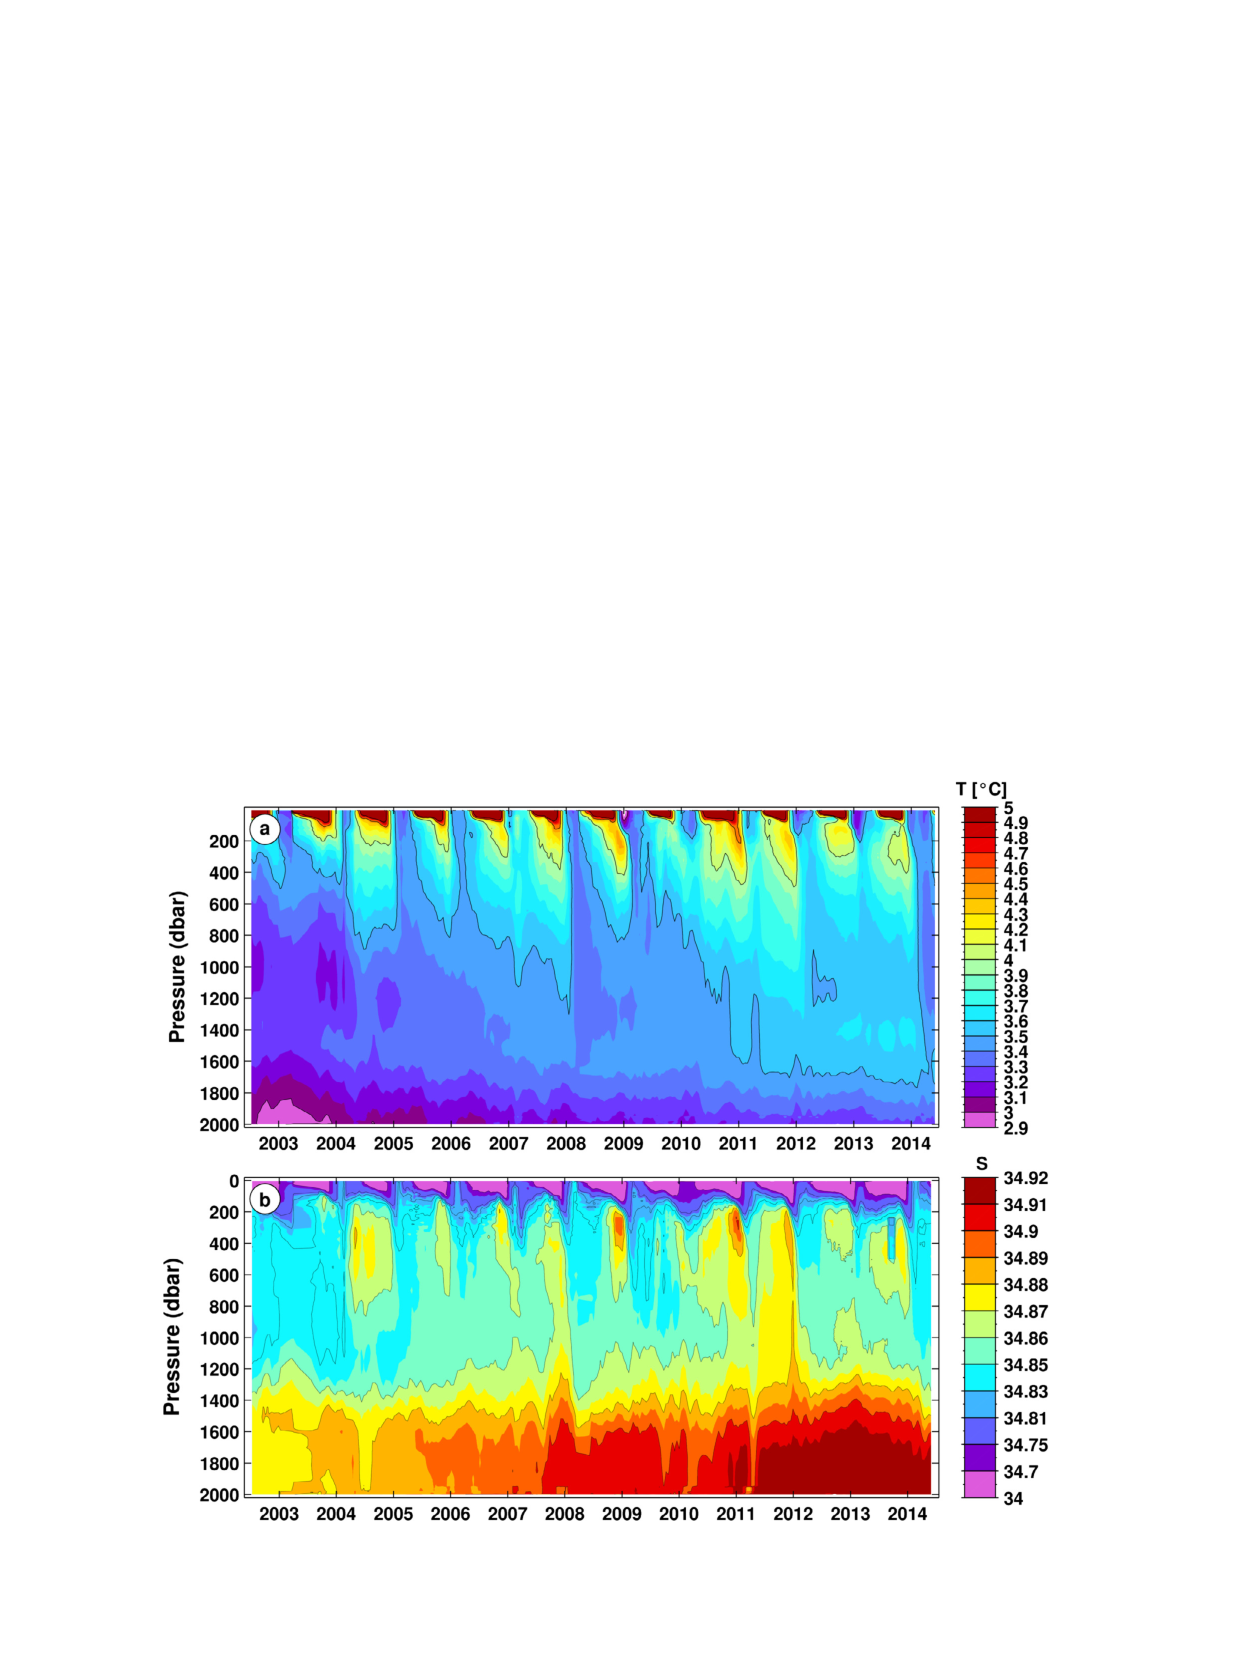
\includegraphics{figs/WaterMasses/KiekeYashayaev15}
    \caption{Time series of convection in the Labrador Sea as measured by autonomous Argo profiling floats \citep{kiekeyashayaev15}}
    \label{fig:KiekeYashayaev15}  
  \end{center}
\end{figure}

This water flows South, hugging the western boundary of the Atlantic ocean in a narrow order 100-km wide flow, that mixes as it goes (\fref{fig:DenglerEtAl06Fig1}).  The boundary current is remarkably persistent, being traced as far south as Florida (\fref{fig:StahrSanford99Fig4}), where bathymetry roughens and disperses the flow.  The flow hugs this side of the basin due to the Coriolis force, and doesn't fall down the slope for the same reason.  Bottom friction does cause it to move downslope slowly, but despite 1600 km of distance between the two sections, its clear that the current hasn't descended very much.  
\begin{figure}[hbt]
  \begin{center}
    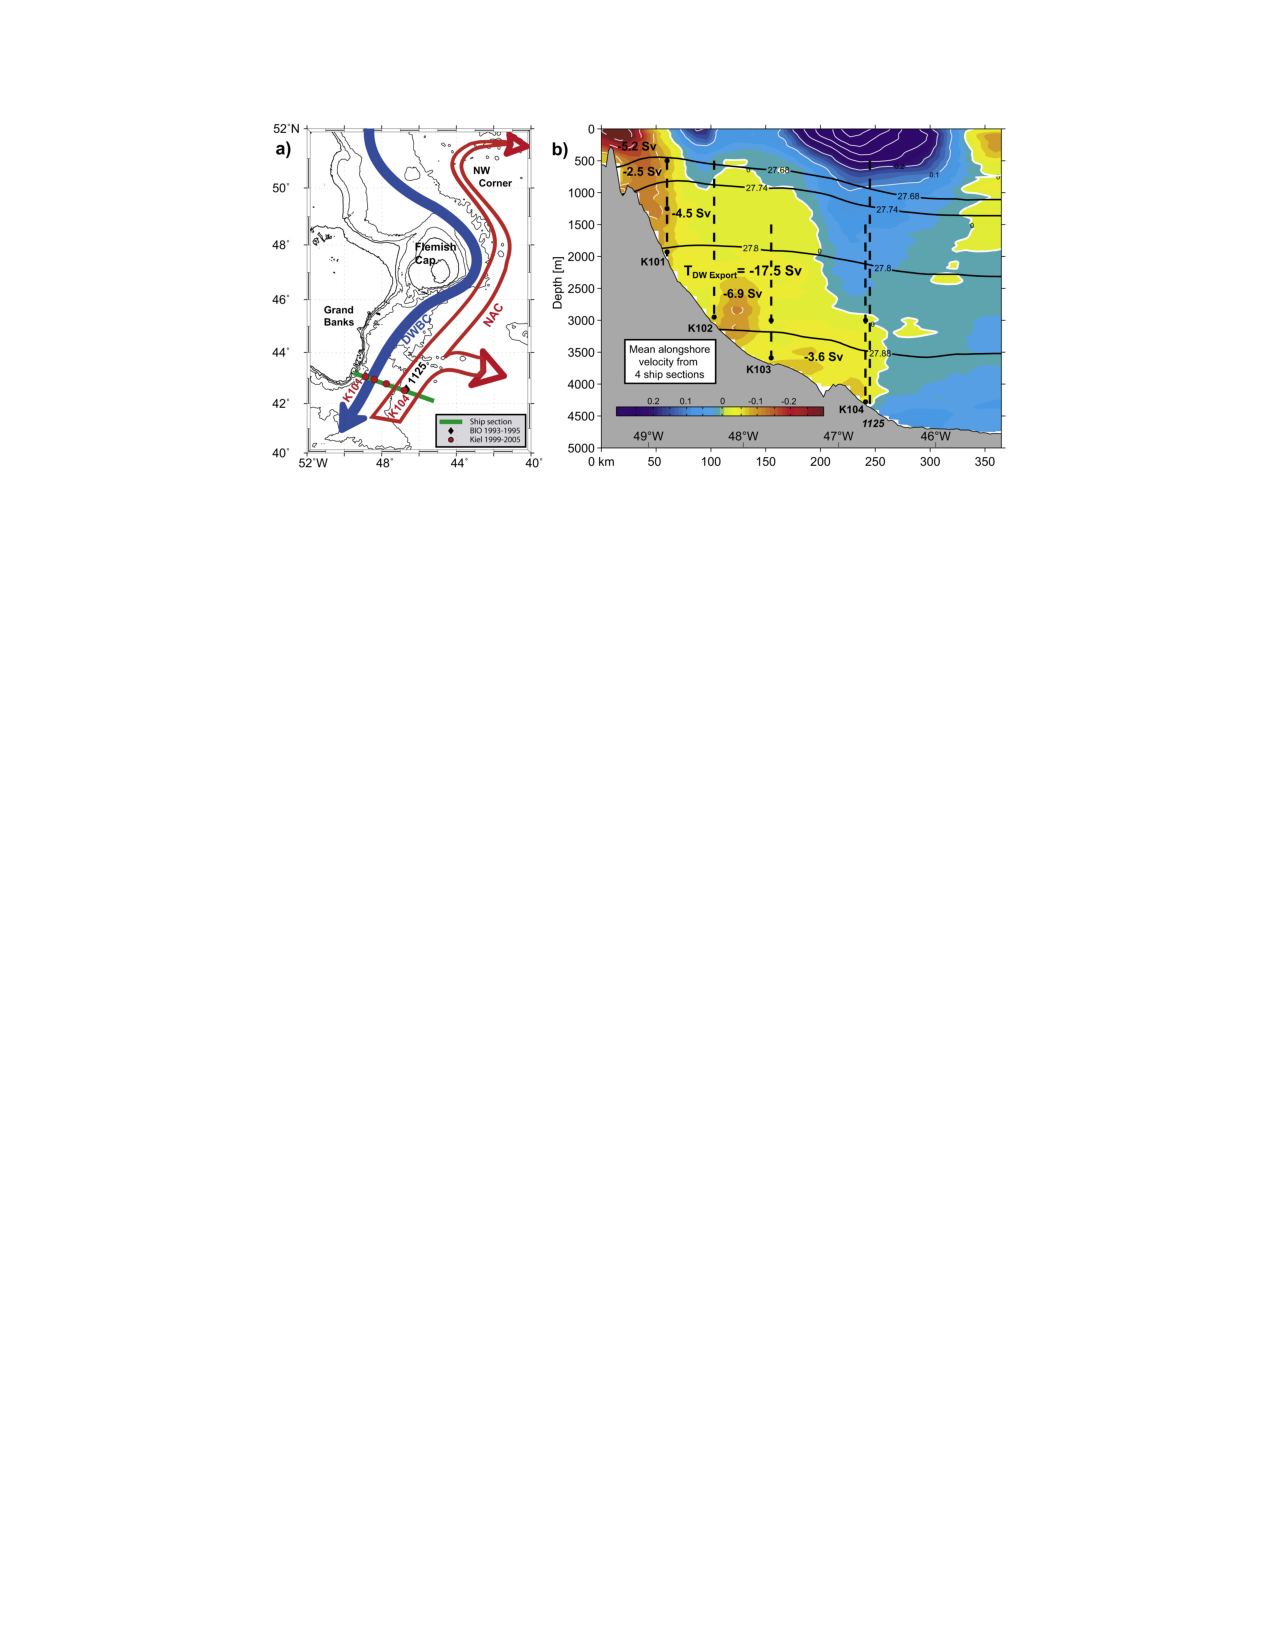
\includegraphics{figs/WaterMasses/DenglerEtAl06Fig1}
    \caption{Observations of Deep Western Boundary Current off the Grand Banks.\citep{schottetal06}}
    \label{fig:DenglerEtAl06Fig1}  
  \end{center}
\end{figure}

\begin{figure}[hbt]
  \begin{center}
    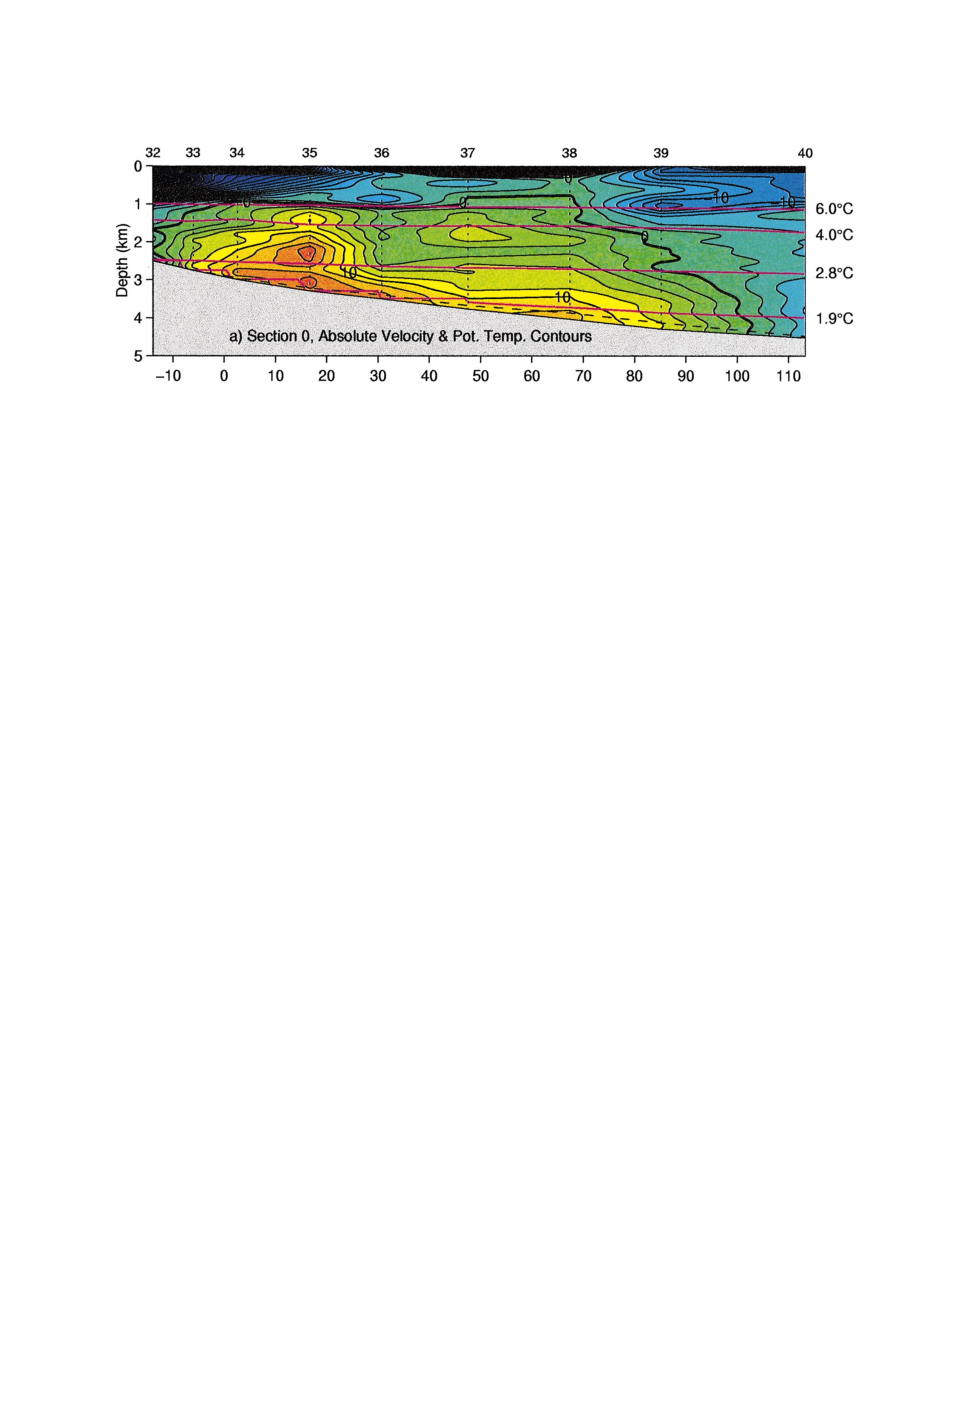
\includegraphics{figs/WaterMasses/StahrSanford99Fig4}
    \caption{Observations of the Deep Western Boundary  Current off Blake Outer Ridge (32 N) \citep{stahrsanford1999}}
    \label{fig:StahrSanford99Fig4}  
  \end{center}
\end{figure}



\section{Inferring the strength of the overturning circulation from data}

The strength of the overturning circulation is almost impossible to infer directly from measuring ocean velocities, and hence it is inferred from ``inversions'' of data collected on hydrographic cruises such as the WOCE and CLIVAR cruises mentioned above.  We haven't discussed geostrophic transport yet, but it will be discussed in future chapters.  However, knowing the density distribution along a section will give us an estimate \emph{within a constant} of the transport of water \emph{across} that section (\fref{fig:SketchCrossSection}.  This somewhat un-intuitive result is because the Coriolis force acting on the moving water balances the pressure gradients.


\begin{marginfigure}
    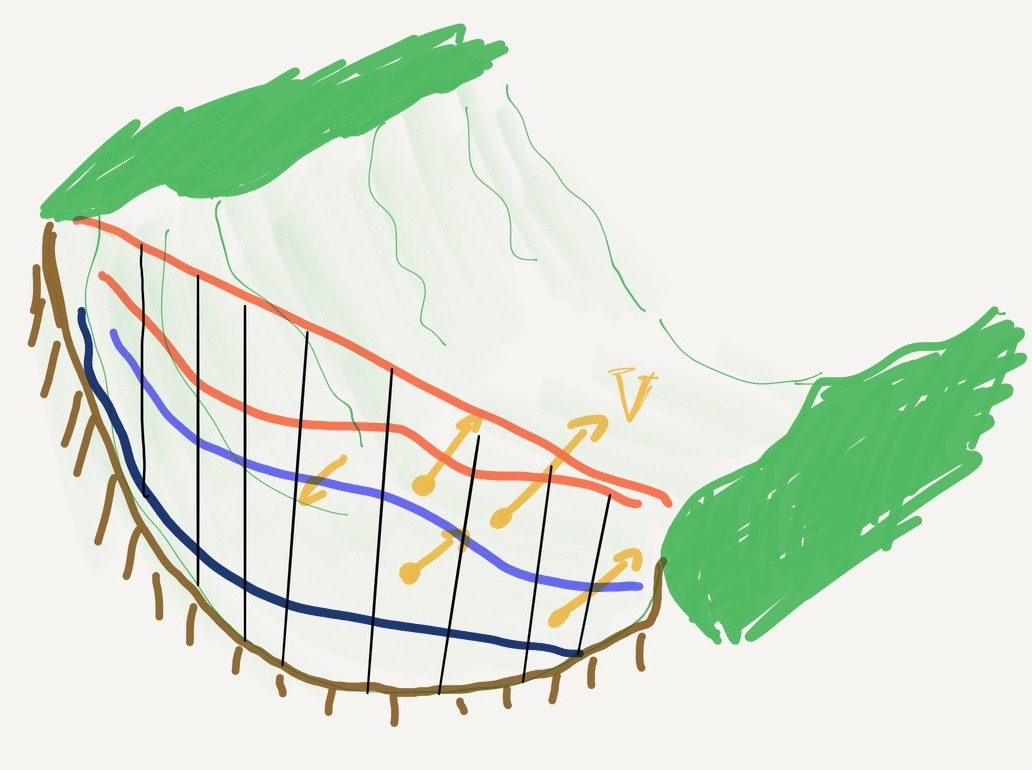
\includegraphics{figs/WaterMasses/SketchCrossSection}
    \caption{Sketch of cross section in a basin.  A hydrographic cruise that has crossed the basin making measurements will give estimates of the pressure gradients along the section, which can be used to estimate the velocity across the section.}
    \label{fig:SketchCrossSection}
\end{marginfigure}


There are unknowns in making these estimates, which can be constrained for by making mass, heat, salt, and other tracers balance in the basins.  We will discuss these results and how they are obtained briefly below.


\subsection{Inverse results}
\label{sec:inverse_results}

The large amounts of data collected during the WOCE and CLIVAR cruises have undergone substantial analysis to determine the strength of the overturning circulation.  The final result is what is described above, but quantified.
Globally, there are two overturning cells, one that sinks in the southern ocean, and the other that sinks in the North Atlantic (\fref{fig:LumpkinSpeer07Fig2}.  The Southern overturning cell is denser and flows under the North Atlantic cell on average.  
(The way these flows are contoured in \fref{fig:LumpkinSpeer07Fig2} may be unfamiliar to some readers, so please see \fref{box:Streamlines}).  

\begin{figure}[hbt]
  \begin{center}
  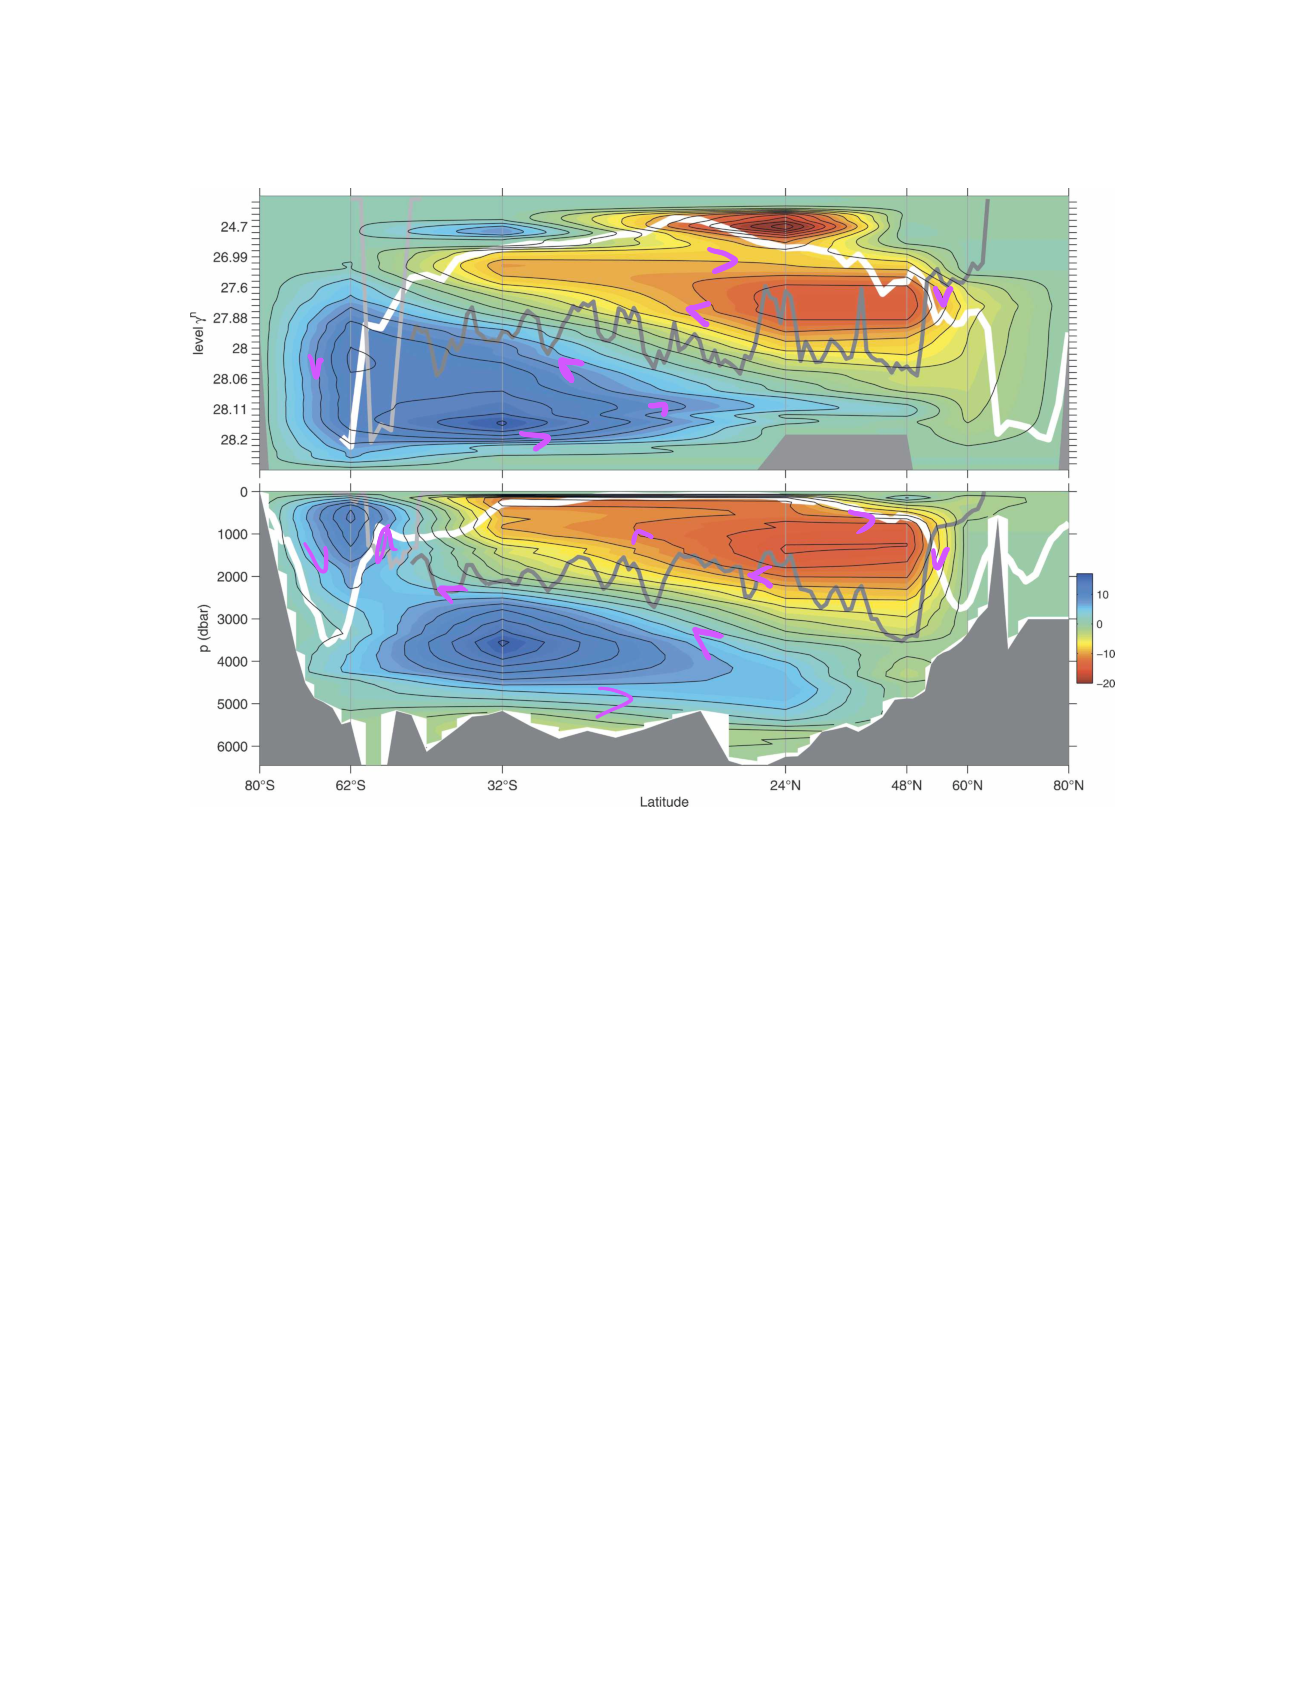
\includegraphics{figs/WaterMasses/LumpkinSpeer07Fig2}
    \caption{Estimate of the strength of the global overturning circulation plotted as a stream function.  The upper plot is the streamfunction plotted with the density of the water as the vertical axes, whereas the lower plot is the depth of the ocean \citep{lumpkinspeer07}.  The stream functions are plotted in units of $Sv$, where $1\,Sv = 10^{6}\ \mathrm{m^3\,s^{-1}}$}
    \label{fig:LumpkinSpeer07Fig2}  
  \end{center}
\end{figure}

\begin{derivbox}[label={box:Streamlines}]{Quantifying flows with streamlines}

A ``streamline'' is a path followed by a parcel in a \emph{steady} flow.  These paths are plotted in 2-dimensions in \fref{fig:LumpkinSpeer07Fig2} and represent the average path of the flow averaged around the world.  This tells us qualitatively where the flow goes.

Streamlines also receive a quantity proportional to the total water transported from the point of the streamline relative to some zero.  So in the sketch below, showing an idealized river, the zero is the southward bank of the river.  The $1\ \mathrm{m^3\,s^{-1}}$ streamline denotes how far across the river you would need to go to get that much downstream (or along streamline) transport.  

\begin{center}
  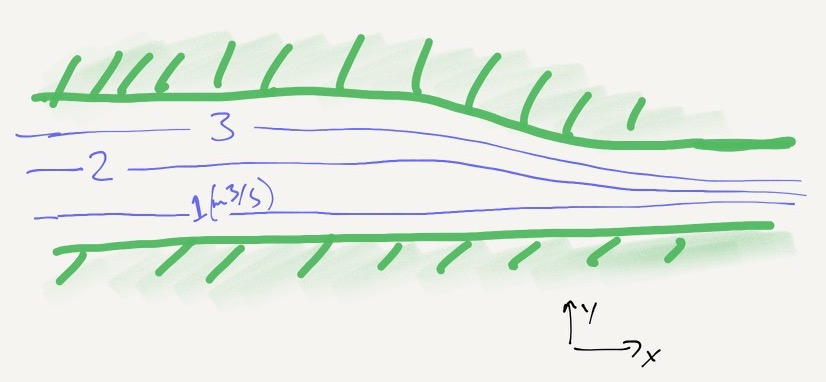
\includegraphics[width=3in]{figs/WaterMasses/SketchStreamline}
    
\end{center}

If the streamlines are drawn so that they have equal transport between them, then the spacing between streamlines is inversely proportional to the speed.  So in the above plot the streamlines get closer together as the river narrows the speed necessarily increases. 

Closed streamlines, as we see above (\fref{fig:LumpkinSpeer07Fig2}) indicate that the flow is circulating around a circuit.  The more streamlines the stronger the recirculation.  

\end{derivbox}

The streamlines look different in the two plots of \fref{fig:LumpkinSpeer07Fig2} because of the different averaging.  However, the absolute values are the same - $20.9 \pm 6.7 \ \mathrm{Sv}$ for the Antarctic Bottom Water cell and $17.2\pm 3.2 \ \mathrm{Sv}$ for the North Atlantic Deep Water cell (the unit $\mathrm{Sv}$ is called a \emph{Svredrup} after Harald Sverdrup and $1\,\mathrm{Sv} = 10^{6}\ \mathrm{m^3\,s^{-1}}$).  

An important reason to plot \fref{fig:LumpkinSpeer07Fig2} with density on the y-axis is to note where mixing is believed to happen.  If water is going down in this reference frame, then it is getting denser, and that must be happening largely due to cooling or mixing with cold water.  If water is going up along this axis it is being warmed by mixing with warm water above.  

There is a stark difference in the overturning circulation between the Atlantic ocean and the Pacific and Indian due to Atlantic Deep Water formation (\fref{fig:LumpkinSpeer07Fig3}).  We see that the deep water in the Atlantic mostly moves south and that there is very little AABW recirculating in that basin.  Conversely, in the Pacific the deep circulation is dominated by the AABW recirculating cell to quite low densities.  


\begin{figure}[hbt]
  \begin{center}
  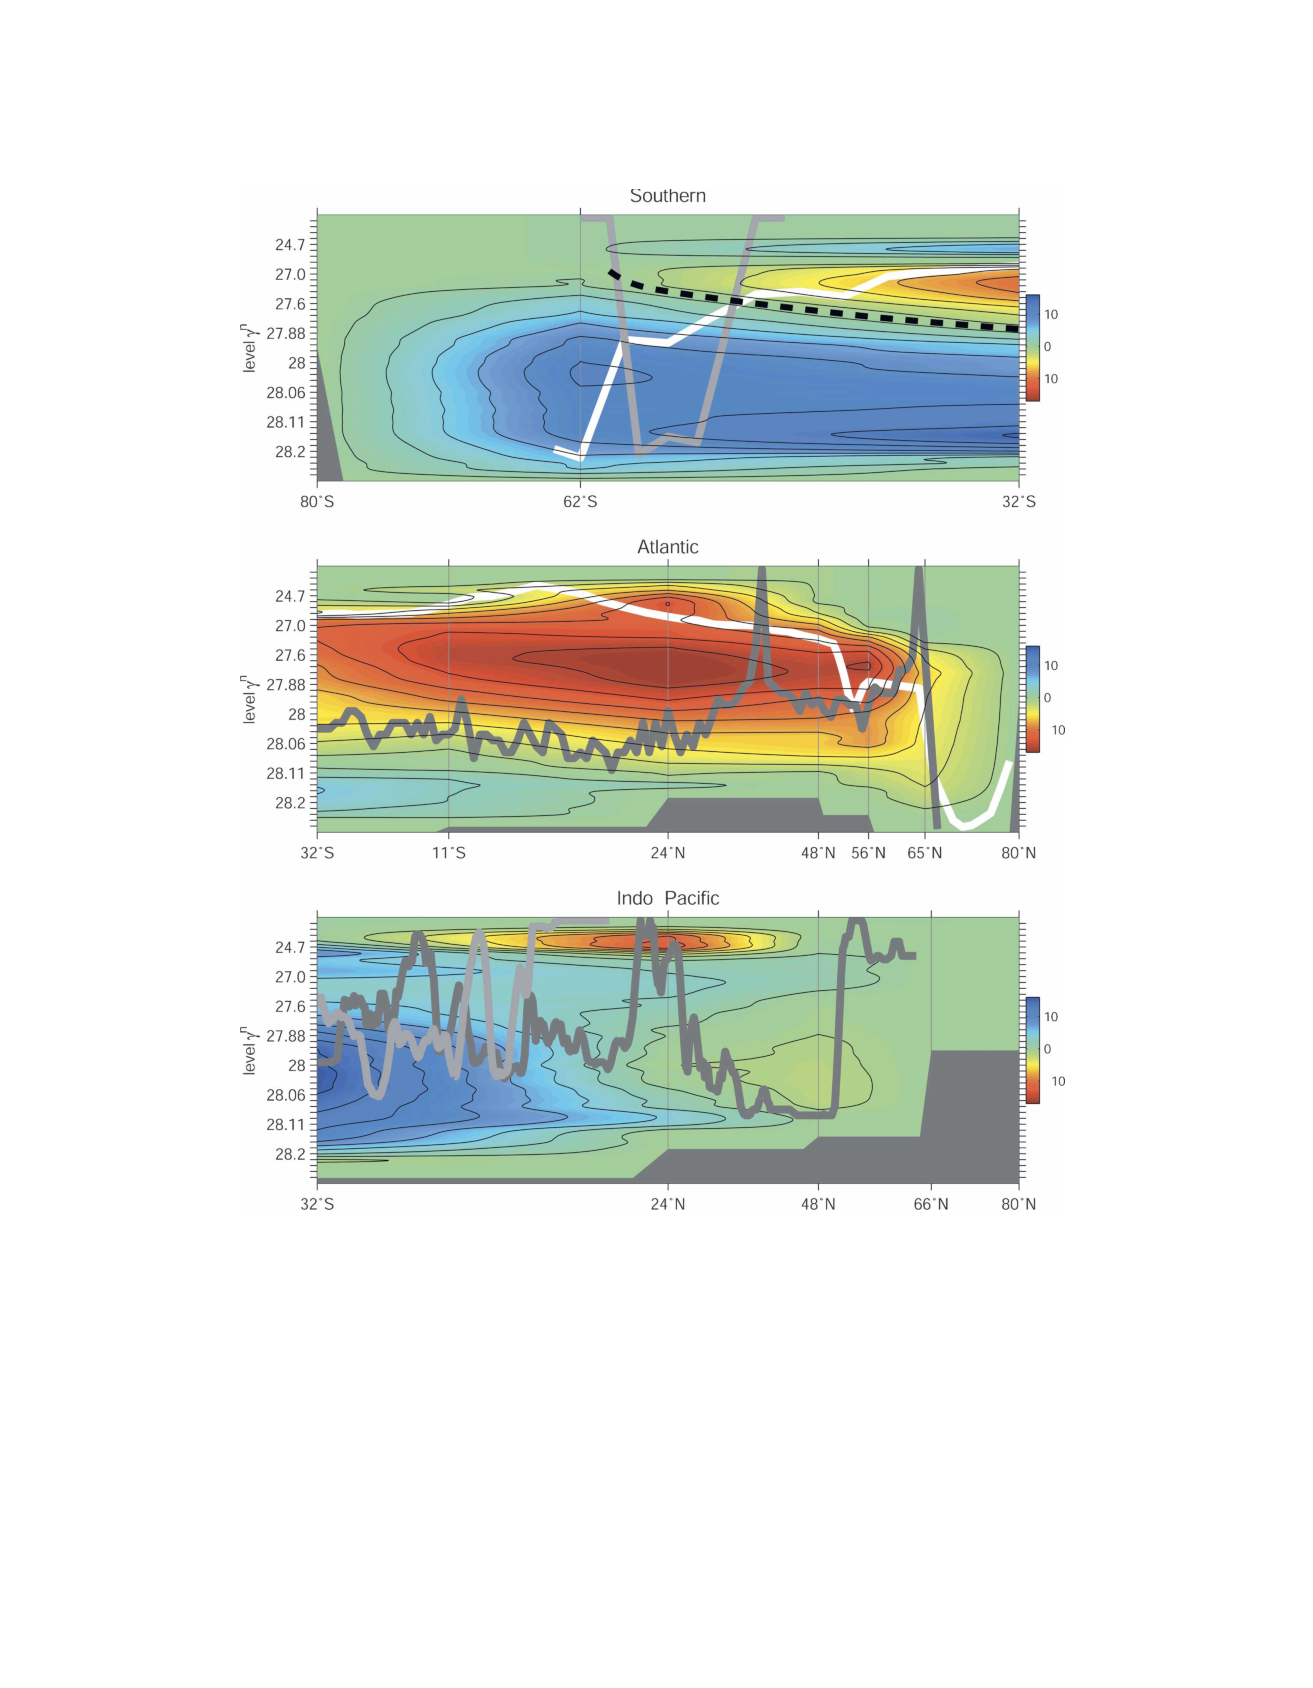
\includegraphics{figs/WaterMasses/LumpkinSpeer07Fig3}
    \caption{As in \fref{fig:LumpkinSpeer07Fig2}, but divided by ocean basin}
    \label{fig:LumpkinSpeer07Fig3}  
  \end{center}
\end{figure}

The strength of the overturning, divided by basin, is shown in \fref{fig:LumpkinSpeer07Fig4}.  The Pacific and Indian each support approximately 10 Sv of upwelling of AABW, while only 5 Sv is upwelled in the Atlantic. However, 17 Sv of NADW is also upwelled in the Atlantic, albeit from a less dense water mass.   There are numerous complicated connections of the water int he upper ocean that must be tracked in order to balance the flux of water, including a very strong exchange between the Indian and Pacific oceans through Indonesia and near Australia.  

\begin{figure}[hbt]
  \begin{center}
  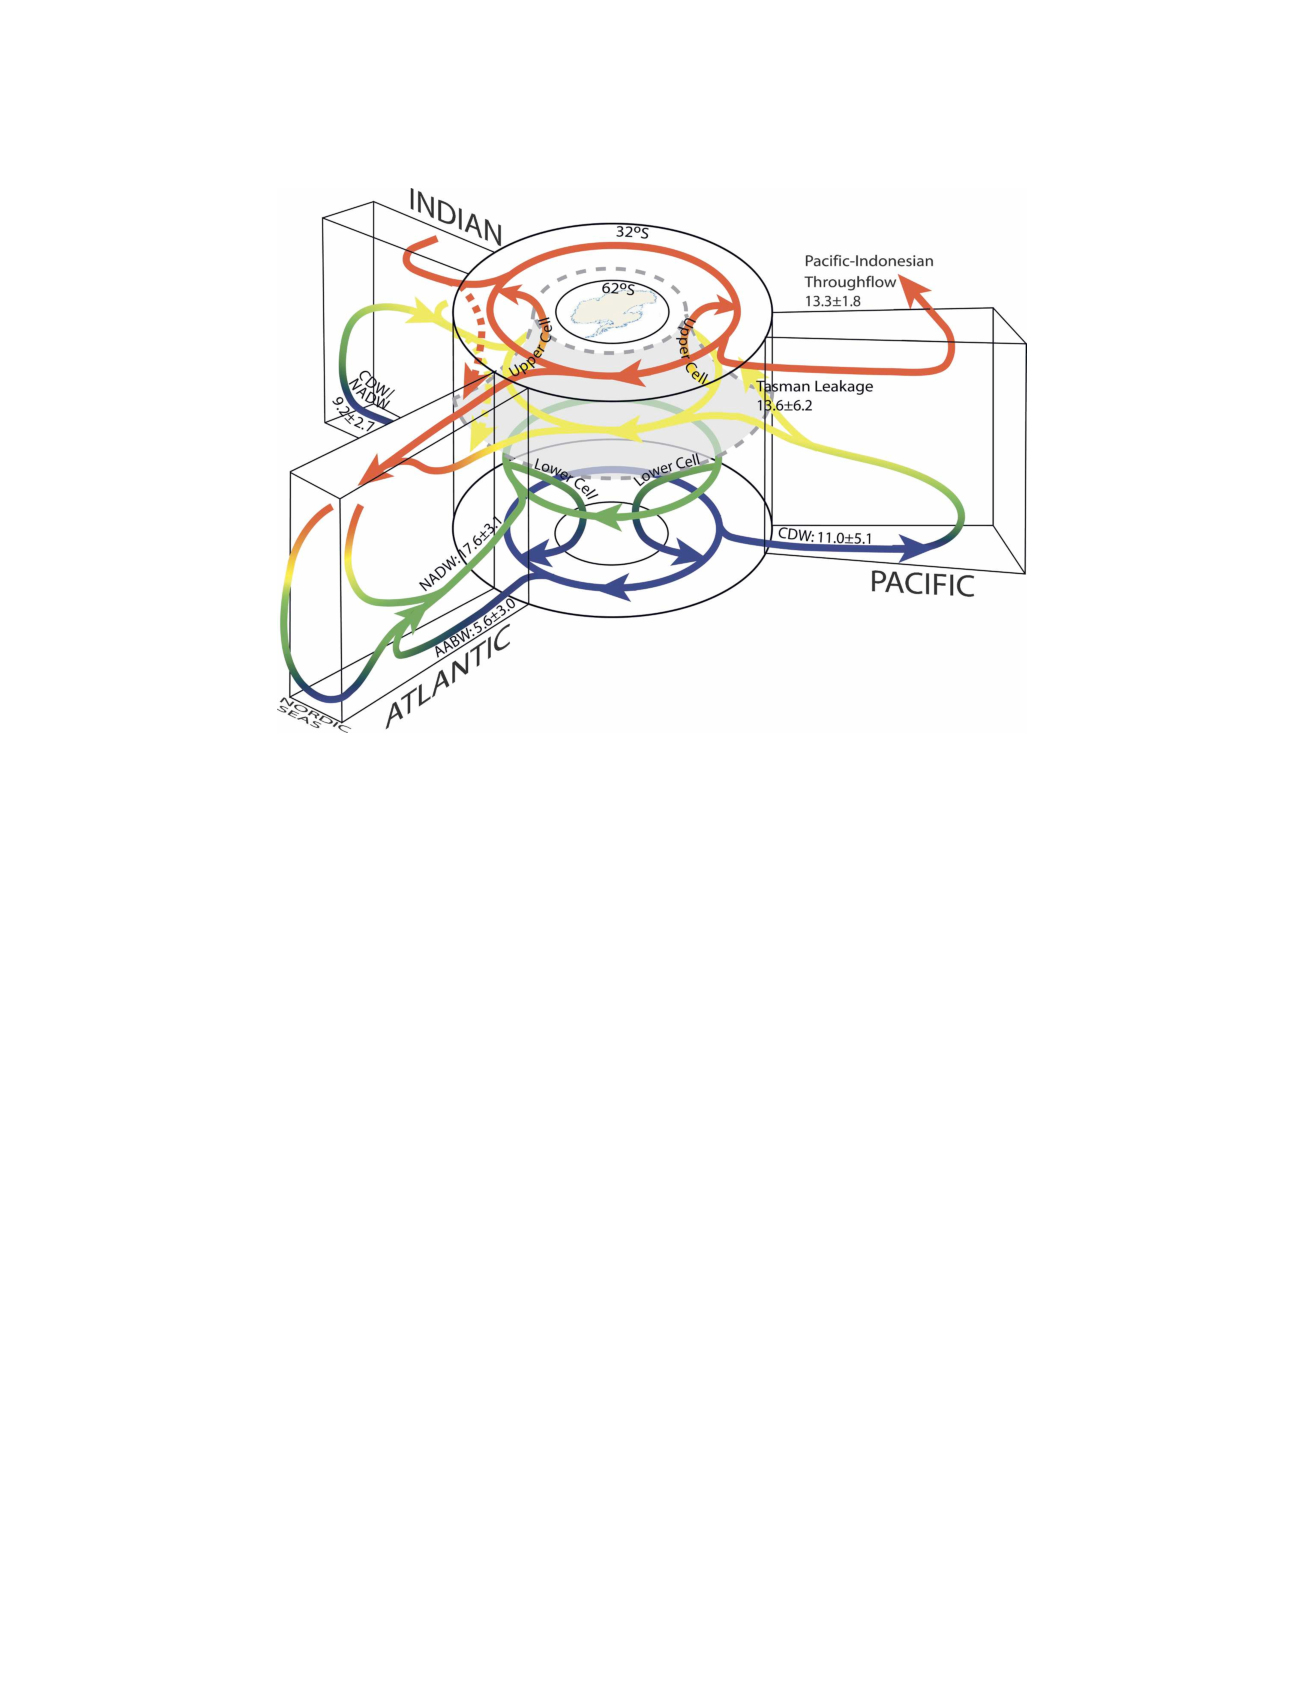
\includegraphics{figs/WaterMasses/LumpkinSpeer07Fig4}
    \caption{Strength of overturning circulation in various basins in $\mathrm{Sv}$.  Blue is the AABW, green is ``deep water'', yellow are ``intermediate'' waters, and orange surface water. \citep{lumpkinspeer07}}.  
    \label{fig:LumpkinSpeer07Fig4}  
  \end{center}
\end{figure}

\subsection{How to make an inverse calculation}

The inverse calculations that go into creating the estimates above are simple in concept, but complicated in execution.  The simplicity comes from just assuming a simple mass balances as we did in previous chapters, and assuming that the ocean is broadly in steady state.  

A very simple example of such an inverse calculation comes from the flow of Antarctic Bottom Water into the Brazil Basin \fref{fig:MorrisEtAl01Fig1}. Water colder than 1 deg C enters in the Vema Channel from the south, but is not observed to make it out of the Brazil Basin.    This can be seen in \fref{fig:MorrisEtAl01Fig4}, where water 1.2-degrees and colder is blocked at the north end of the basin.  

Channels like the Vema Channel are nice, because the flow can be  monitored with moorings, which was done in the late 70s \citep{hoggetal82} and again late 90s \citep{morrisetal01}.  These moorings found, on average, 3.7 Sv of water flowed in the channel that was colder than 1.2 degrees \citep{morrisetal01}.  This water, on average, is 0.2 degrees-C.  

\begin{figure}[hbt]
  \begin{center}
    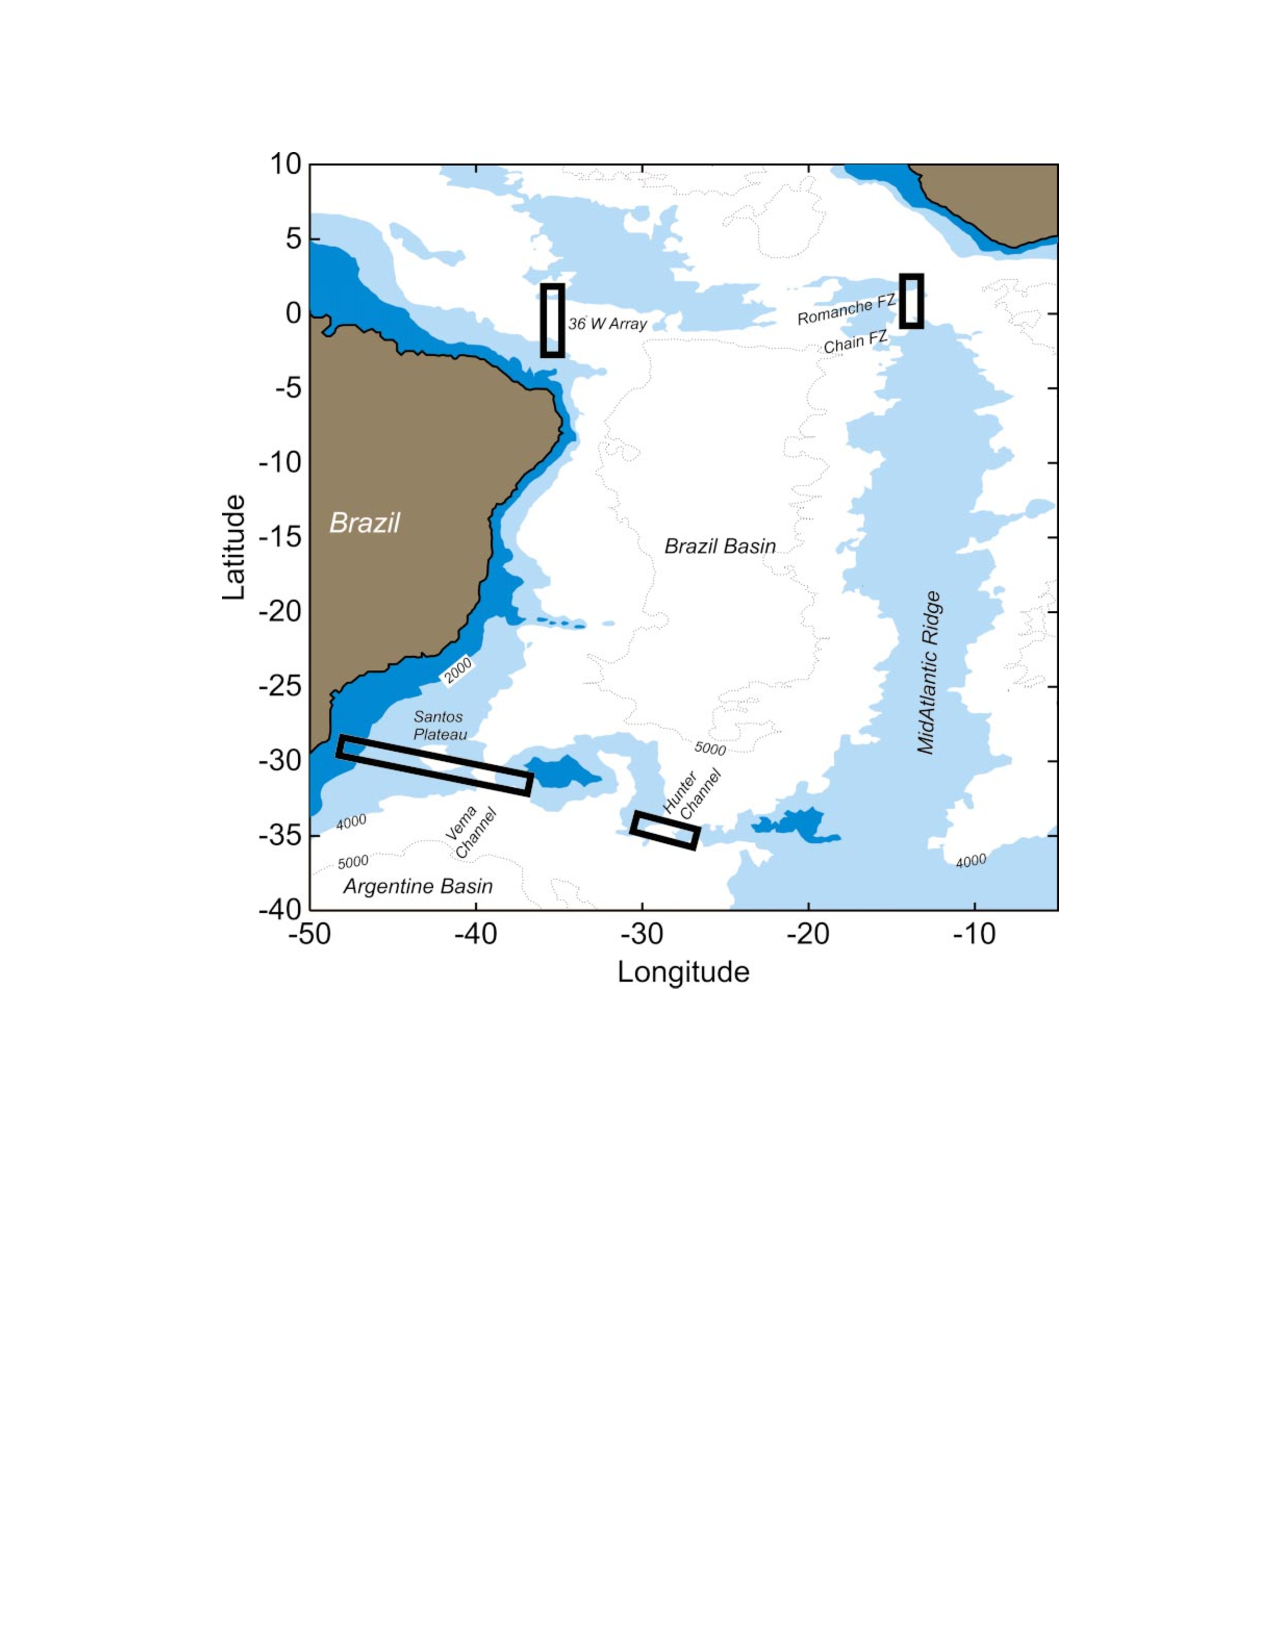
\includegraphics[width=3in]{figs/WaterMasses/MorrisEtAl01Fig1}
    \caption{Map of the Brazil Basin \citep{morrisetal01}}
    \label{fig:MorrisEtAl01Fig1}  
  \end{center}
\end{figure}
\begin{figure}[hbt]
  \begin{center}
    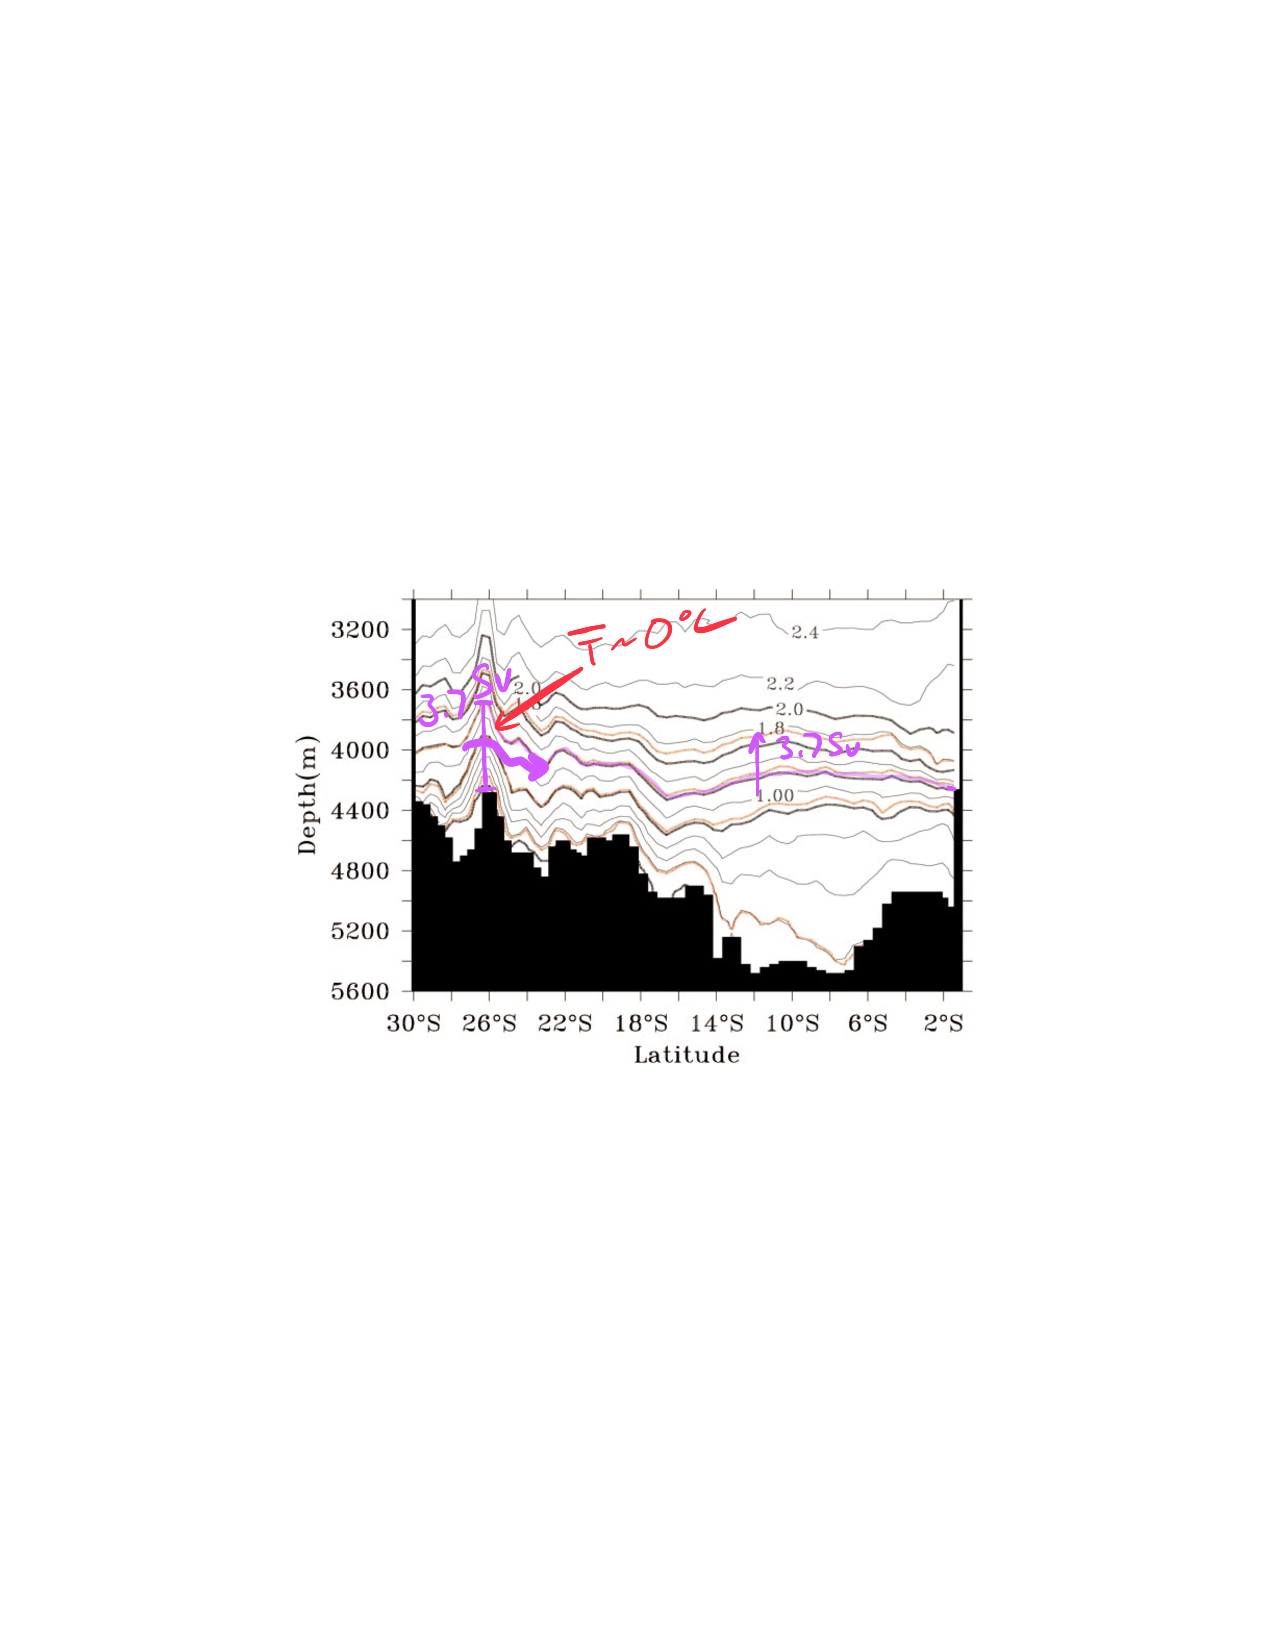
\includegraphics{figs/WaterMasses/MorrisEtAl01Fig4Ann}
    \caption{Hydrography along the Brazil Basin.  Note that water colder than 1.2 degrees C does not make it out the north end.   \citep{morrisetal01}}
    \label{fig:MorrisEtAl01Fig4}  
  \end{center}
\end{figure}

We can apply a volume budget and a heat budget to the problem, by considering a volume bounded by the Vema channel at the south, the north end of the Brazil Basin, and the 1.2 degree isotherm at the top.  The volume budget is straight forward - if 3.7 Sv enters in Vema Channel and there is no outlet to the north, it must cross the 1.2 degree isotherm.  $Q_{in} = Q_{out}$.  

The heat budget is almost the same, but we need to include the heating due to diffusion at the top of our volume:
\begin{equation}
    h_{in} + h_{diffusion}= h_{out}
\end{equation}
where $h_{in} \approx  3.7 \mathrm{Sv}\, 0.0 \mathrm{C} = 0 \mathrm{Sv\,C}$, and $h_{out} \approx 3.7 \mathrm{Sv}\, 1.2 \mathrm{C} = 4.4 \mathrm{Sv\,C}$.  This means that the residual has to come into the volume via diffusion:
\begin{equation}
    h_{diffusion} = K \frac{d\theta}{dz} A    
\end{equation}
where $\frac{d\theta}{dz}$ is the average vertical temperature gradient at the top of the volume, and $A\approx 7\times10^{12}\mathrm{m^2}$ is the area of the 1.2 degree isotherm in the basin.  There were lots of hydrographic cruises made in the Brazil basin, such that the gradient was found to be 
$\frac{d\theta}{dz}\approx 2.1\times10^{-3}\mathrm{C\,m^{-1}}$. This leaves us with only one unknown, $K$, the turbulent diffusivity necessary to mix the temperature gradient fast enough to counter the cold water coming into the basin from the south.  And carrying out the math, we get a final answer of $K\approx 3\times10^{-4}\ \mathrm{m^2s^{-1}}$.   \citet{morrisetal01} divide the water in the basin into more layers and determine that the turbulent diffusivity is between 2 and $3\times 10 ^{-4}\ \mathrm{m^2\,s^{-1}}$ .  Note that this is over 1000 times the molecular diffusivity of heat, so turbulence must be responsible for this inferred mixing.  

The amount of turbulence required to maintain such a high turbulent diffusivity is moderately strong.  Field work was carried out there to measure the turbulence directly using instruments called \emph{shear probes}, which are 1-cm scale phonograph needles encased in a silicone tip.  The results show that there is indeed substantial mixing in the Brazil Basin, but that it is not at all homogeneous, with the strongest mixing occurring on the east side where there is substantial roughness (\fref{fig:PolzinEtAl97Fig2}).  Indirect evidence is that this heightened mixing is due to tides moving back and forth over the rough bathymetry and creating turbulence with the stratified water above.  Note that in most of the basin, even above the rough topography, the turbulence is substantially \emph{lower} than the mean inferred from the inverse calculation.  However, the mean is dominated by the few red and orange pixels in the data, and there are enough of those that the average comes out to $0.5-1.5\times10^{-4}\ \mathrm{m^2\,s^{-1}}$ \citep{polzinetal97}.  This is within a factor of two of the inverse estimate, and probably within error bounds of both.  It is also likely that the Brazil Basin is undersampled by the turbulence measurements and there is some mixing ``hot spots'' that the sampling missed.   

\begin{figure}[hbt]
  \begin{center}
  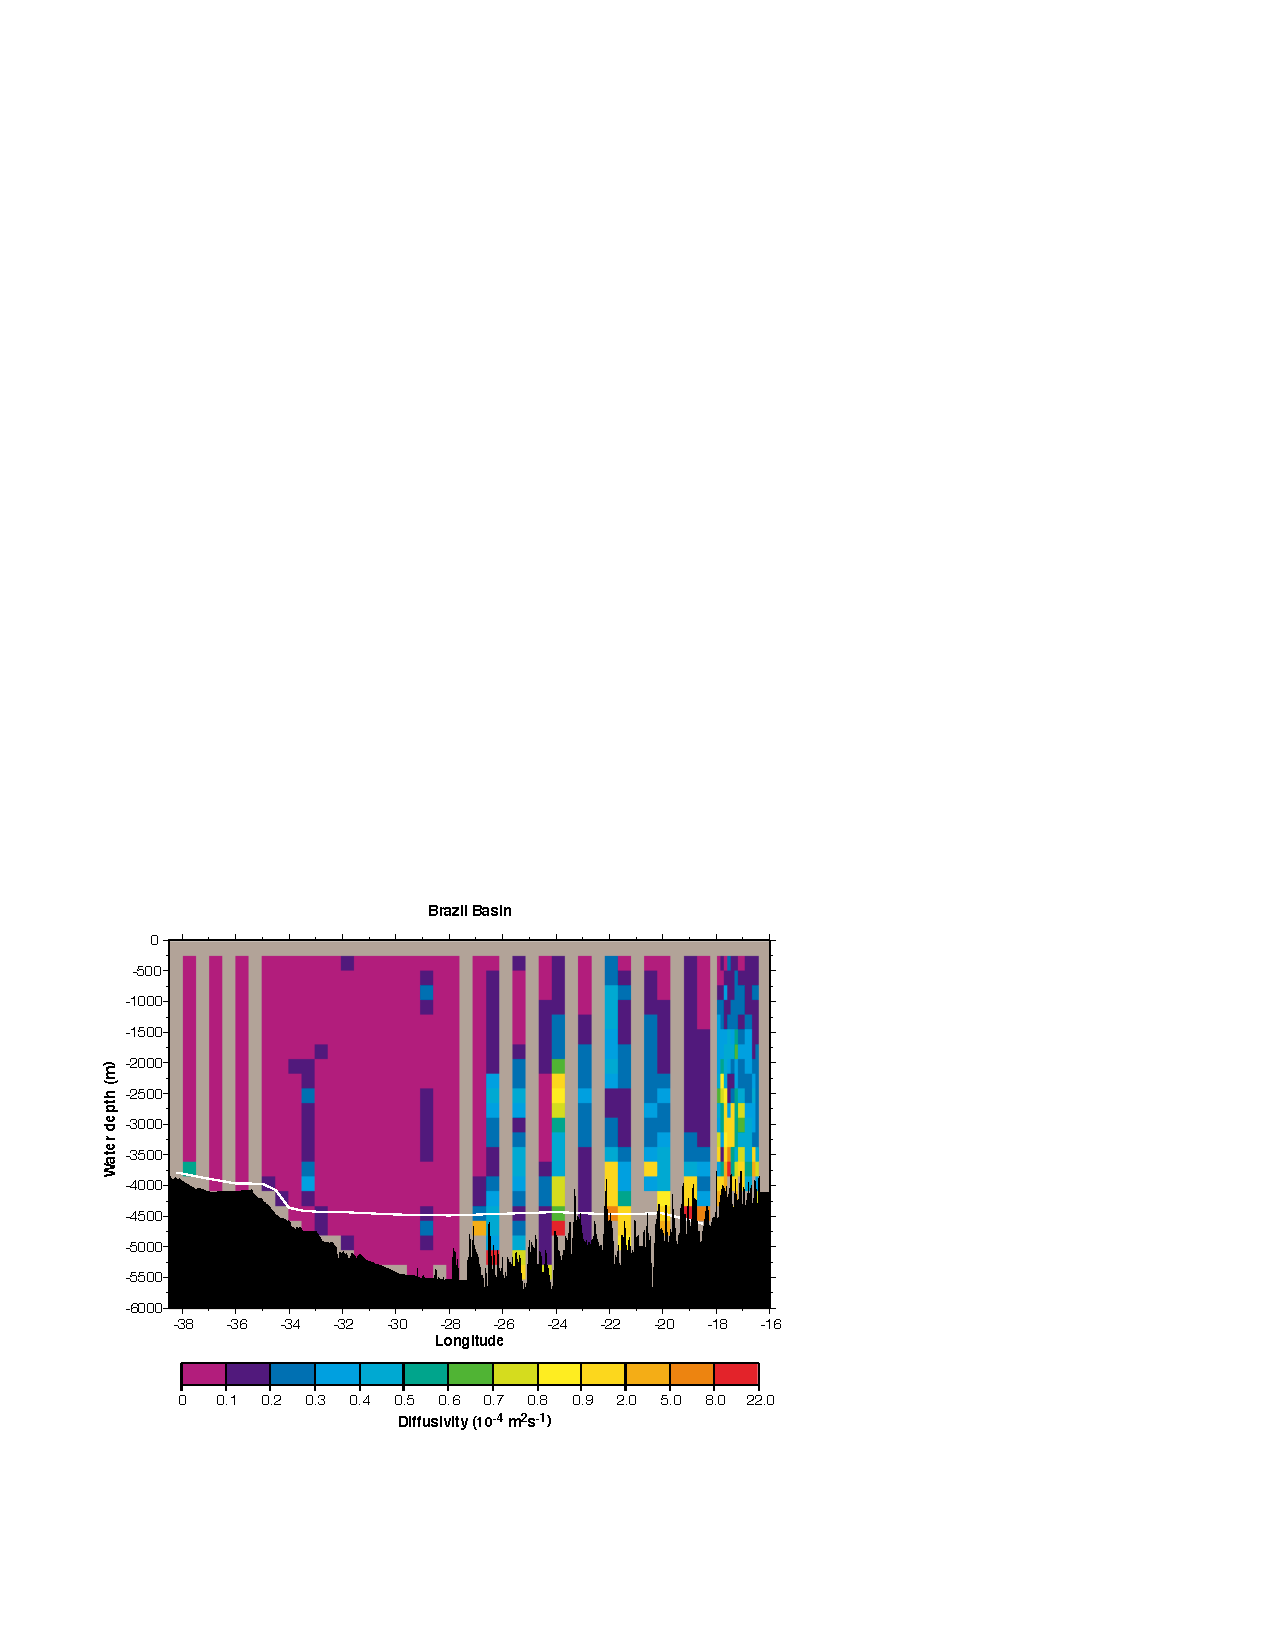
\includegraphics{figs/WaterMasses/PolzinEtAl97Fig2}
    \caption{Turbulence diffusivity inferred from directly measuring turbulence.  The cross section is made west-to-east across the Brazil Basin, and the 0.8-degC isotherm is shown in white. \citep{polzinetal97} }
    \label{fig:PolzinEtAl97Fig2}  
  \end{center}
\end{figure}

Extending the inverse estimate made in the Brazil Basin to the global oceans is exactly what was done in \fref{sec:inverse_results}.  Volumes of the ocean were constrained by the cross-basin cruises. However, in addition to an unknown diffusivity in the ocean, there were unknown offsets in the velocity measurements (because we do not have current meters everywhere in the ocean), and sampling errors due to temporal variability.  So, what is done for global estimates is to use substantially more data from other tracers.  These tracers have their own uncertainties; for instance silicate is used, but the accumulation of silicate in the deep ocean is an unknown.  C14 is used, but will be biased by particles raining down from the surface ocean.  These data and unknowns are all put into a large matrix, and then then the best solutions for the unknowns are inverted for by minimizing error in all the individual constraints.  This was the procedure pioneered by \citet{wunsch96}, and followed by \citet{lumpkinspeer07} in the results above.

\section{Theory of overturning circulation and Sandstrom's theorem}

From the above, we might have the idea that the overturning circulation is driven by how much cold water you make.  Thats true to an extent - the heating gradient between the poles and the equator is one part of what drives the overturning circulation, and plus or minus any net heating or cooling, the heat transport in the ocean must balance the hating differential (\fref{fig:SketchHeatingCooling}).  

\begin{marginfigure}
    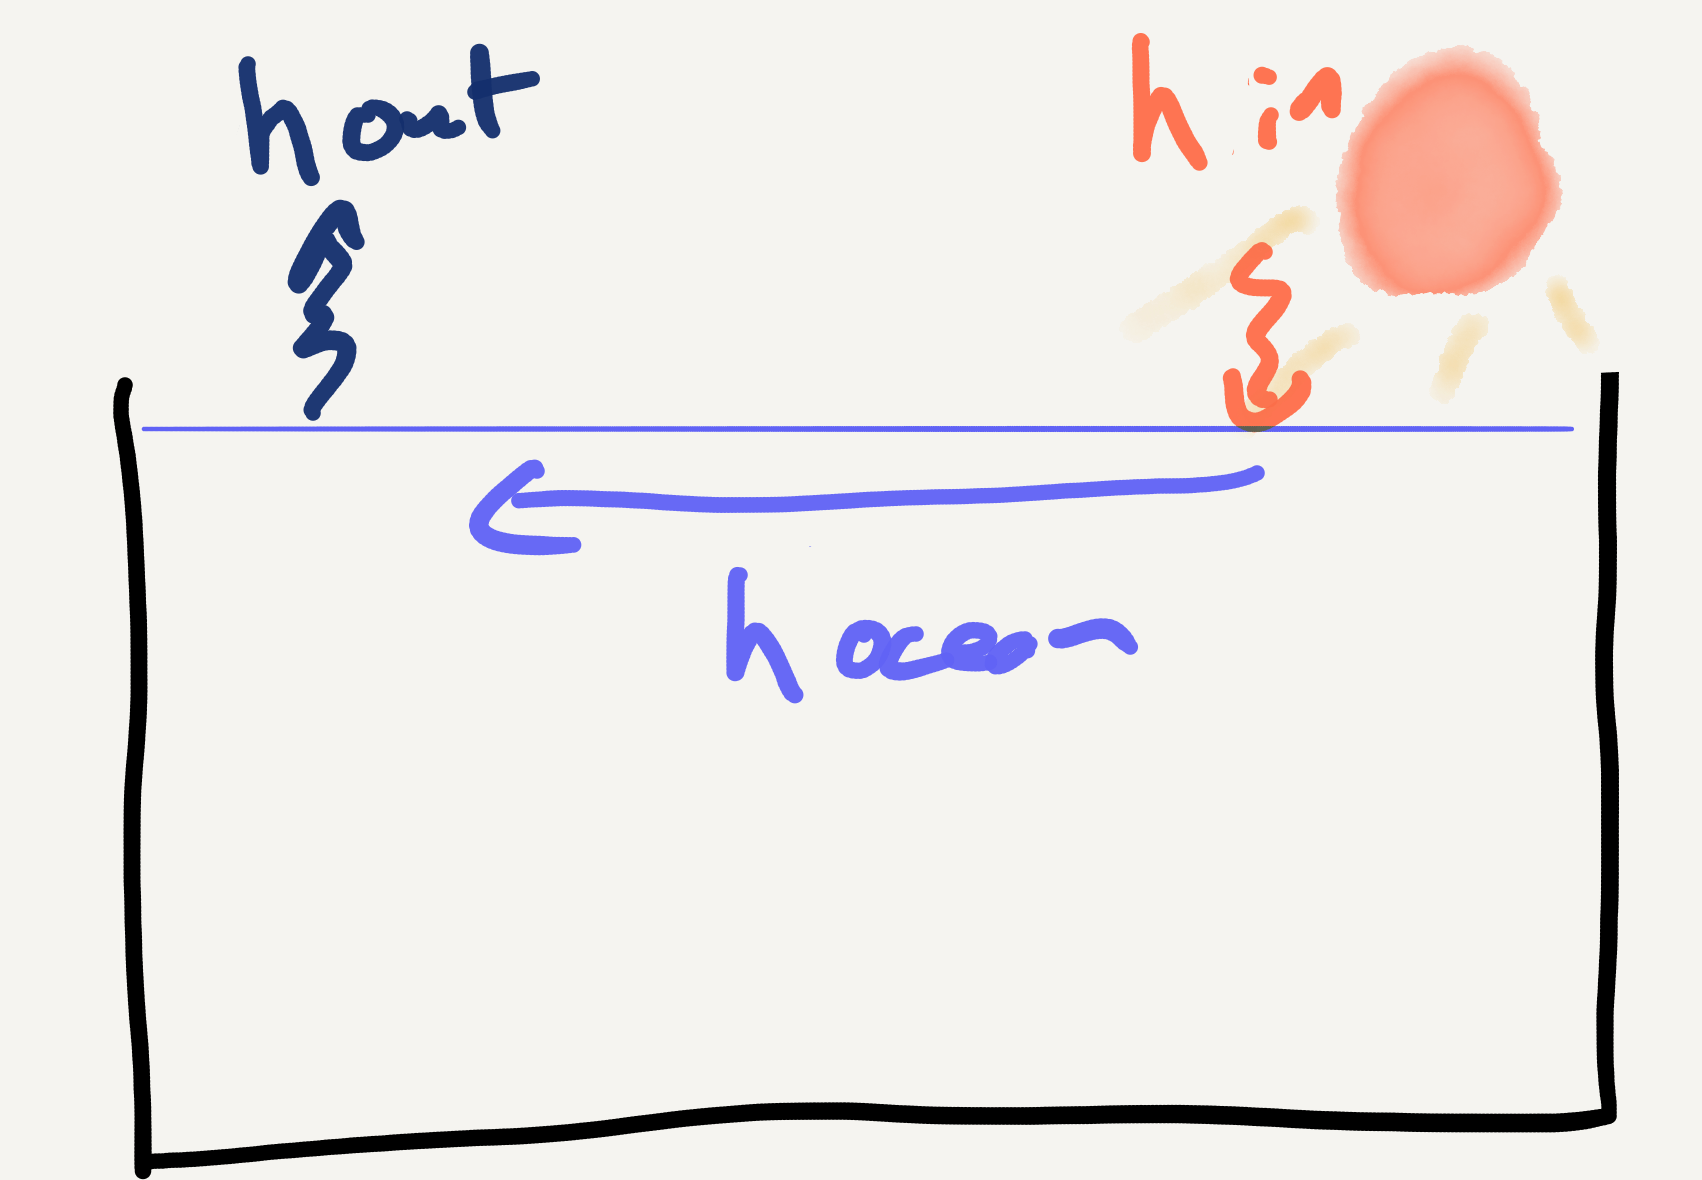
\includegraphics{figs/WaterMasses/SketchHeatingCooling}
    \caption{Sketch of heat input into a one-pole ocean.  The heat flux in must be balanced by the heat flux out, and the ocean must transport that heat from the equator to the poles.}
    \label{fig:SketchHeatingCooling}  
\end{marginfigure}

However, just like a river pouring into an estuary, its possible for that heat flux to be carried in a very shallow current and drive a very weak volume transport that only affects the very surface ocean.  In such a world, all the deep ocean would be very cold, and a thin layer at the surface would be very warm (\fref{fig:SketchMixing}).

So for a given heat difference at the surface, what ultimately drives the strength of the overturning circulation is how strong mixing is in the ocean.  By mixing the heat down, the ocean creates lateral density gradients, and lateral gradients create lateral pressure gradients that ultimately drive circulation (\fref{fig:SketchMixing}).  

\begin{marginfigure}
    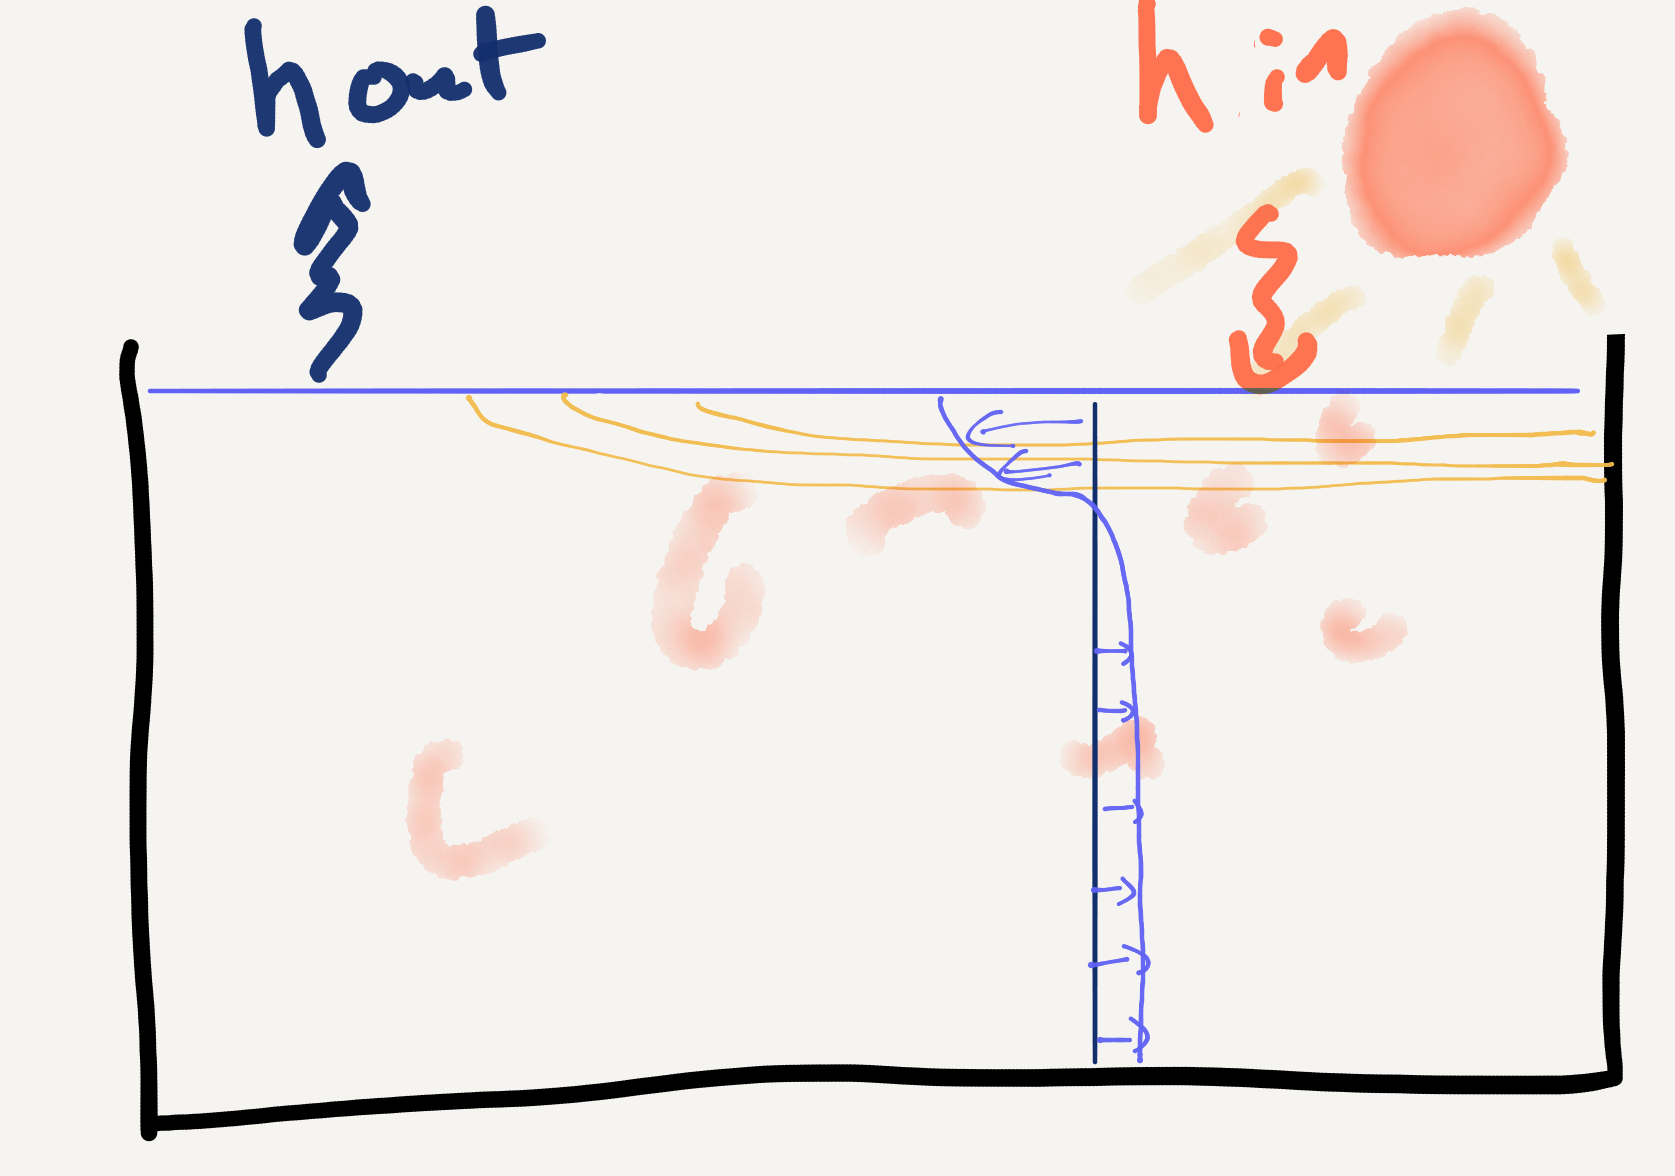
\includegraphics{figs/WaterMasses/SketchWeakMix}
    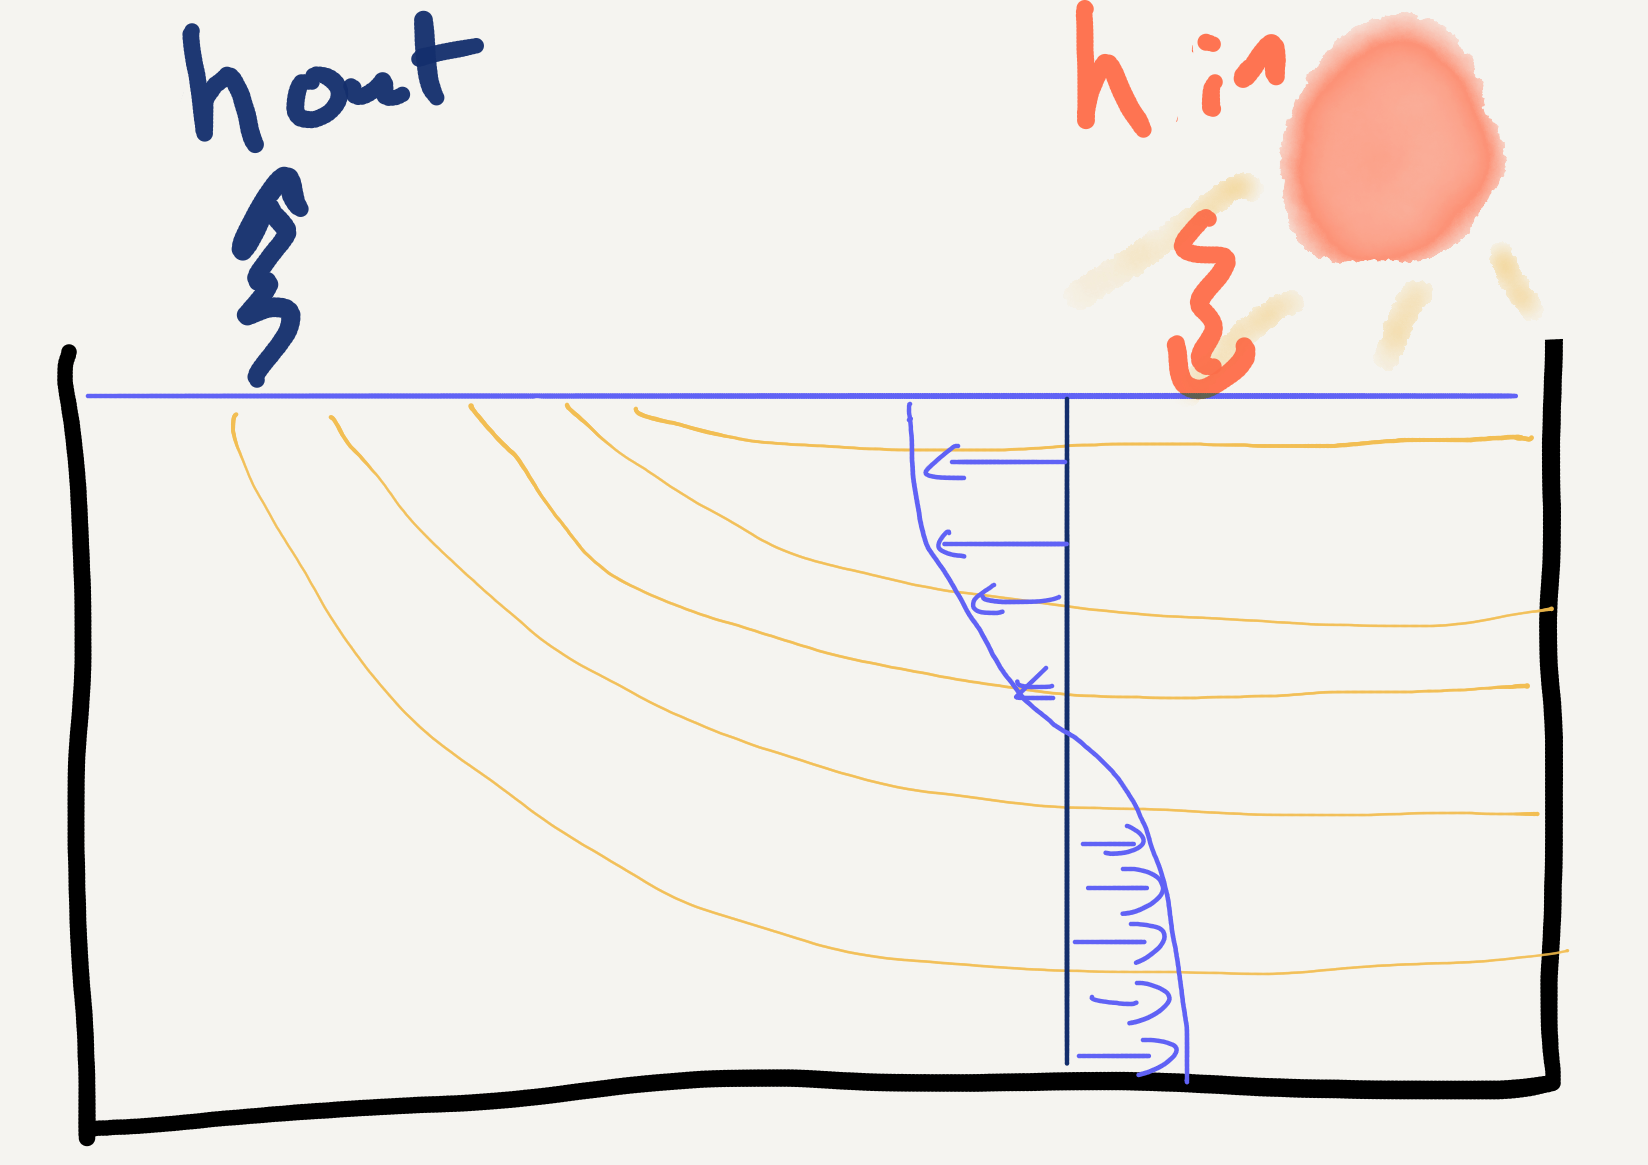
\includegraphics{figs/WaterMasses/SketchStrongMix}
    \caption{Sketch of two different oceans with the same external heat differential.  The top panel shows weak mixing, and the bottom panel shows strong mixing.  The heat transports from equator to pole are the same, but the amount of circulation is much stronger in the second case.}
    \label{fig:SketchMixing}  
\end{marginfigure}

The other way to think of this is to think of the \emph{potential energy} of the system.  Recall from previous chapters that the isopycnals surfaces in \fref{fig:SketchMixing} want to flatten out.  This means that tilted isopycnals have potential energy that they would not have if the isopycnals were all flat.  This idea of potential energy and the need to mix buoyancy to depth in the ocean is nicely encapsulated by \emph{Sandstrom's theorem} which states that heating and cooling at the same depth will not drive a vigorous circulation in fluid.  Essentially surface heating and cooling does not increase the potential energy of the system, and hence there is no strong circulation driven.

Conversely mixing of heat down from the equatorial regions \emph{does} increase the potential energy.  However, it is important energetically to realize that this mixing cannot arise because of the overturning circulation itself.  i.e. the 20-30 Sv of overturning noted above cannot create the turbulence that drives the overturning.  This would be the equivalent of the ocean lifting itself by its own bootstraps.  Instead the energy for the overturning circulation must come from other sources of deep ocean mixing.  This again is directly analogous with the situation in an estuary - the estuarine circulation is catalyzed by mixing in the estuary.

This dependence of the overturning circulation on the strength of the turbulence has been tested numerically.  Stronger mixing transports heat deeper in the ocean (\fref{fig:Bryan87Fig3}) making for stronger lateral gradients.  This drives a more vigorous overturning circulation (\fref{fig:Bryan87Fig7}).  The scaling of the overturning circulation with the vertical diffusivity $K$ is approximately $K^{1/3}$ (\fref{fig:Bryan87Fig8}).  These integrations were carried out many years ago, but the basic results have held up well to more sophisticated treatments.  

\begin{figure}[hbt]
  \begin{center}
  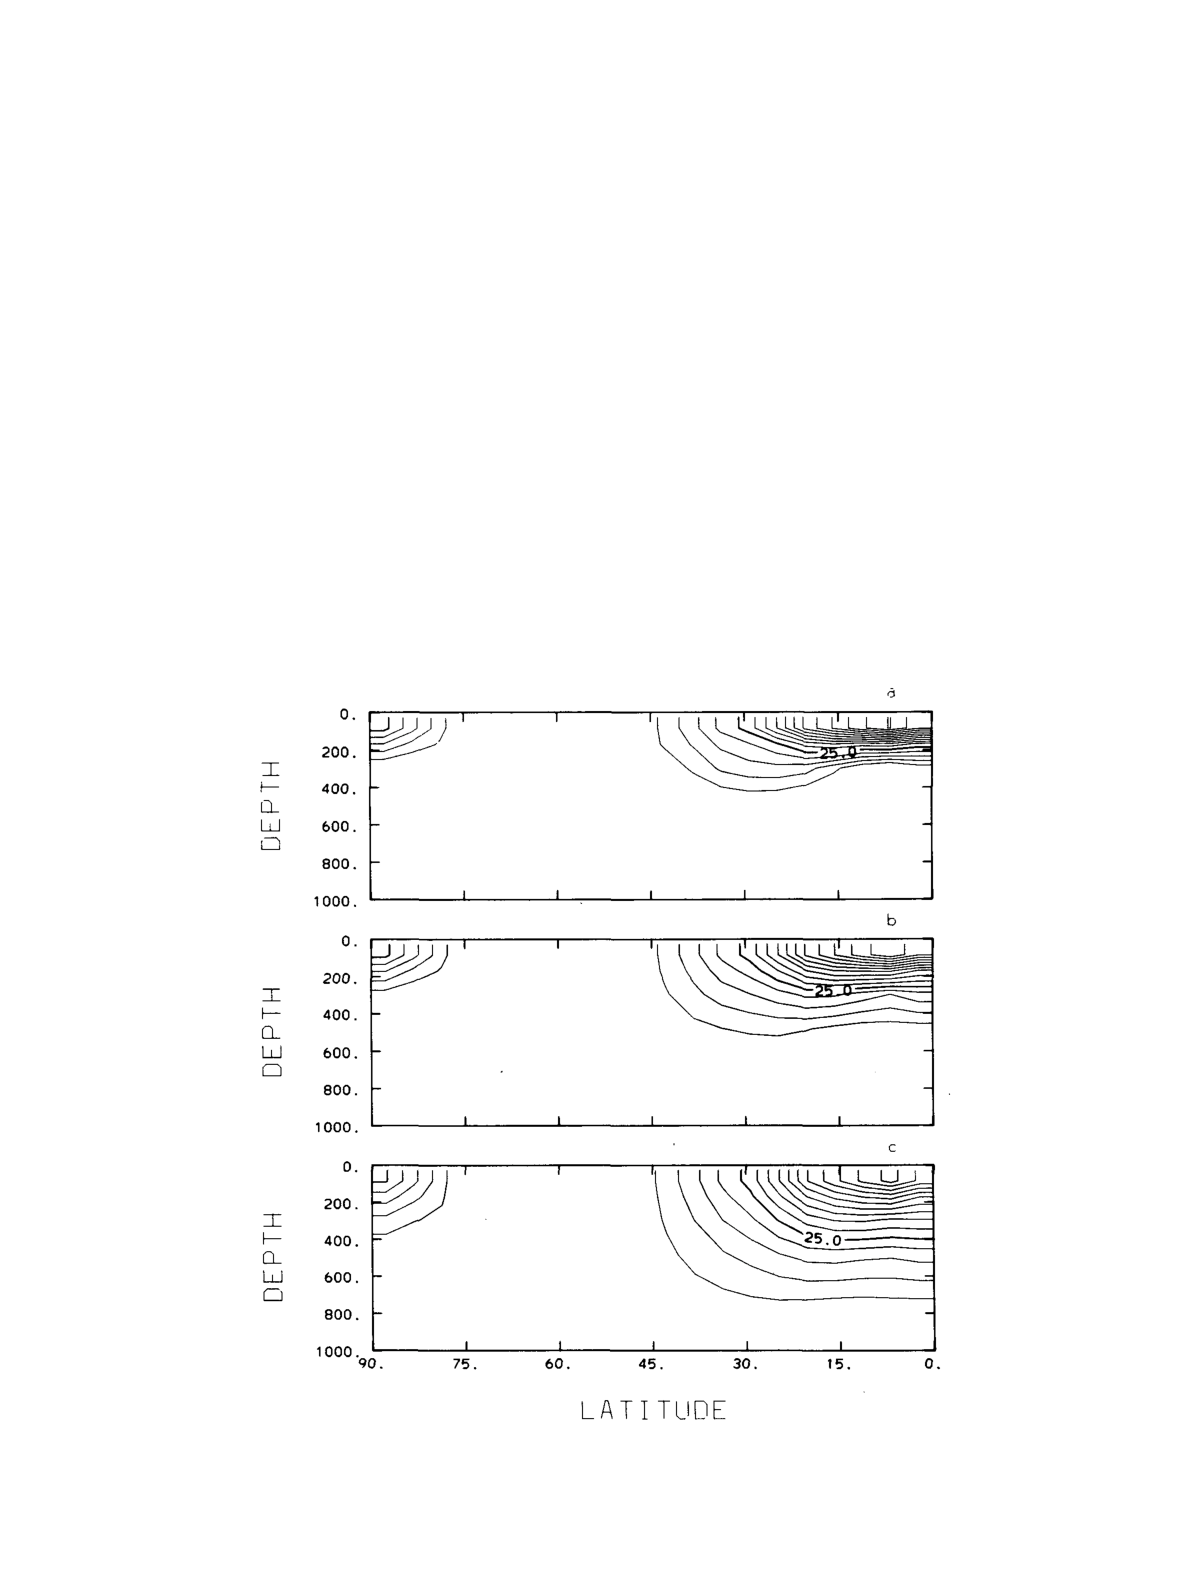
\includegraphics[width=2.1in]{figs/WaterMasses/Bryan87Fig3}  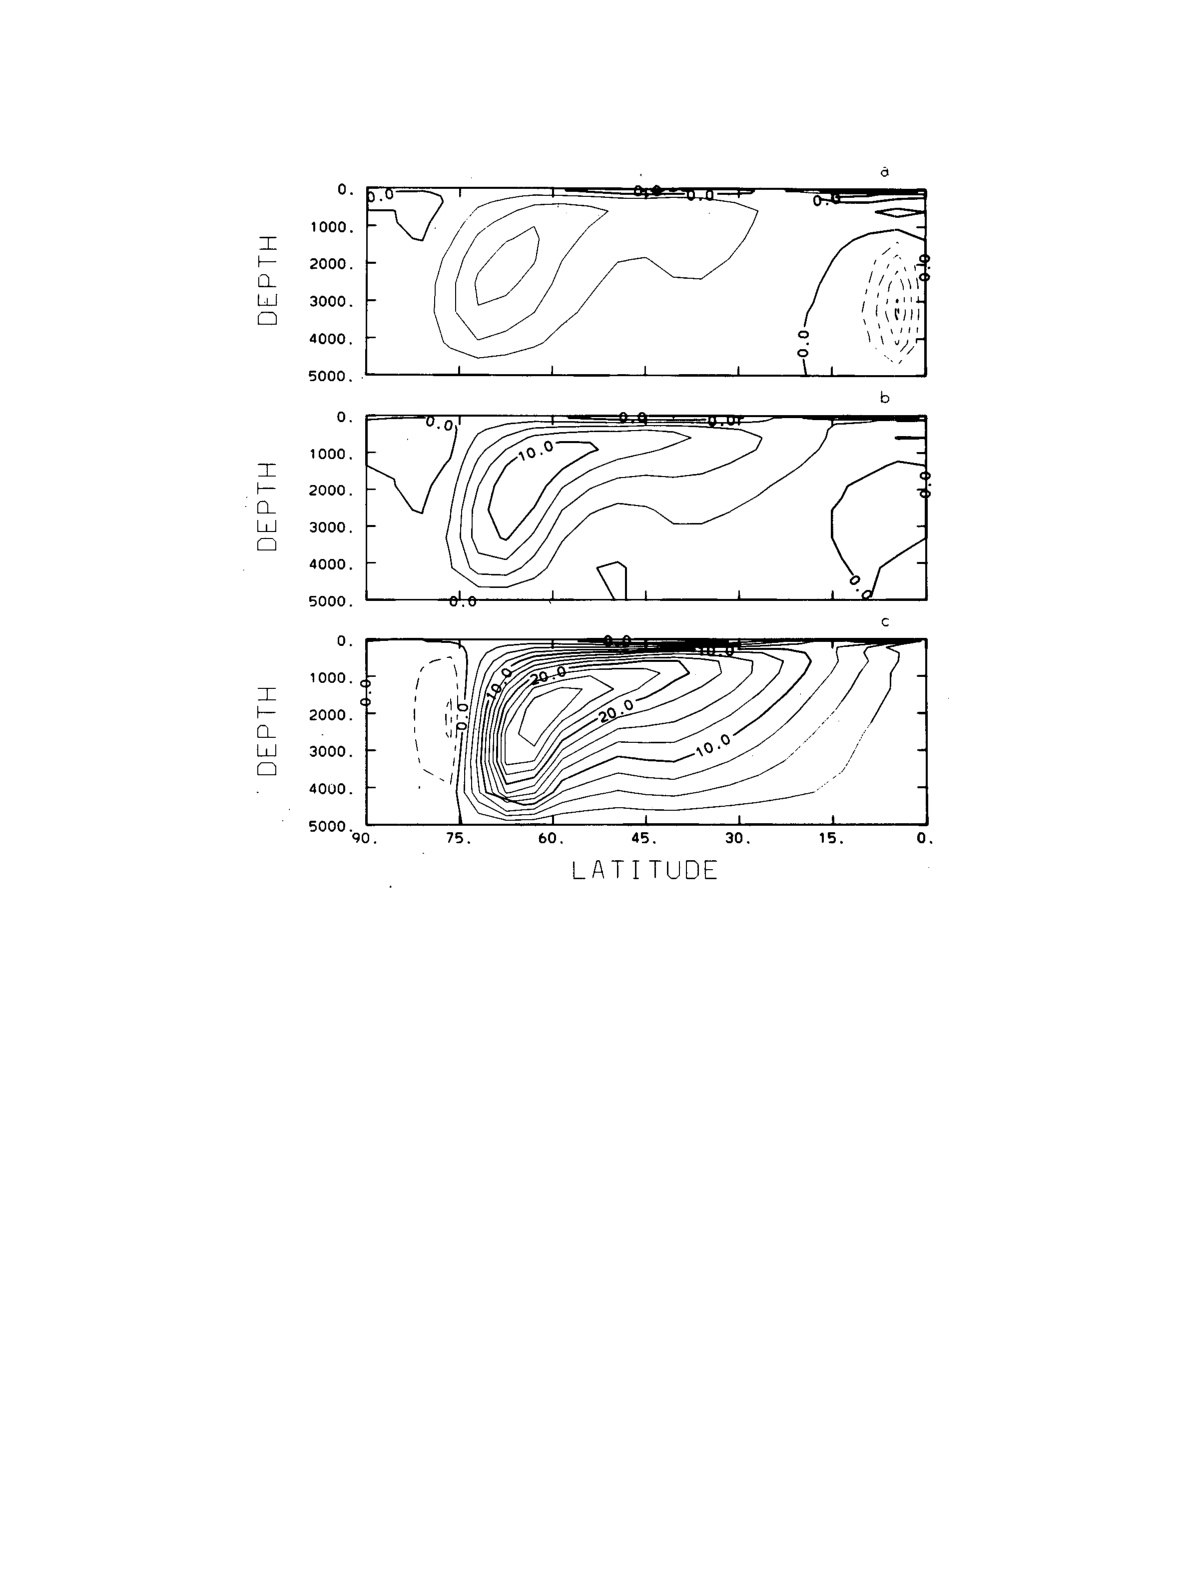
\includegraphics[width=2.1in]{figs/WaterMasses/Bryan87Fig7}
      \caption{Left panels: Potential temperature cross section in a numerical ocean with different vertical diffusivities: $0.1, 0.5$ and $2.5\times10^{-4}\mathrm{m^2\,s^{-1}}$.  Right panels: Overturning streamfunctions.  \citep{bryan87}}
    \label{fig:Bryan87Fig3}  
  \end{center}
\end{figure}

\begin{figure}[hbt]
  \begin{center}
  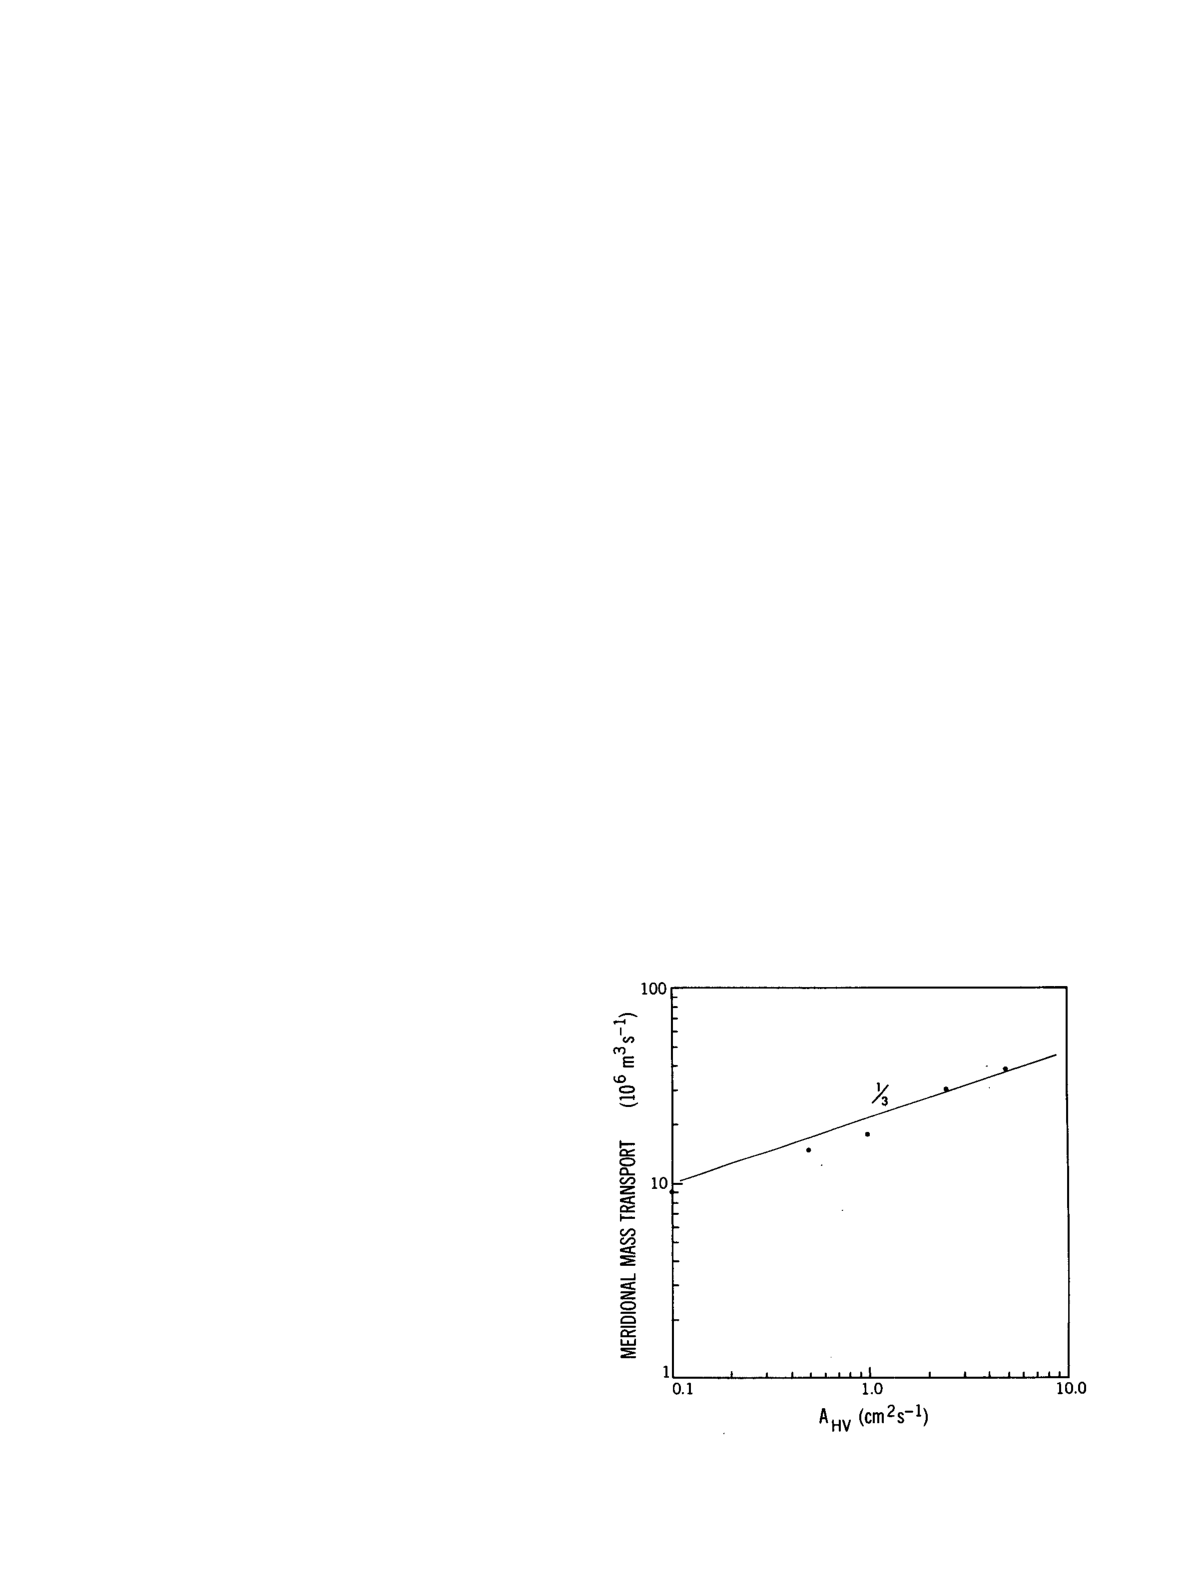
\includegraphics[width=2in]{figs/WaterMasses/Bryan87Fig8}
      \caption{Dependence of the overturning circulation strength on the vertical diffusivity used in the idealized model \citep{bryan87}.}
    \label{fig:Bryan87Fig8}  
  \end{center}
\end{figure}

The tides and wind are believed to be the energy source for the mixing that drives the overturning circulation.  Because the fluid is stratified, energy is able to radiate into the interior from the boundaries as \Wikiref{internal waves}.  There are many sources and pathways of internal waves, and their importance to the overturning circulation has catalyzed a significant research into their properties (\fref{fig:MacKinnonEtAl17Fig1}).

\begin{figure}[hbt]
  \begin{center}
    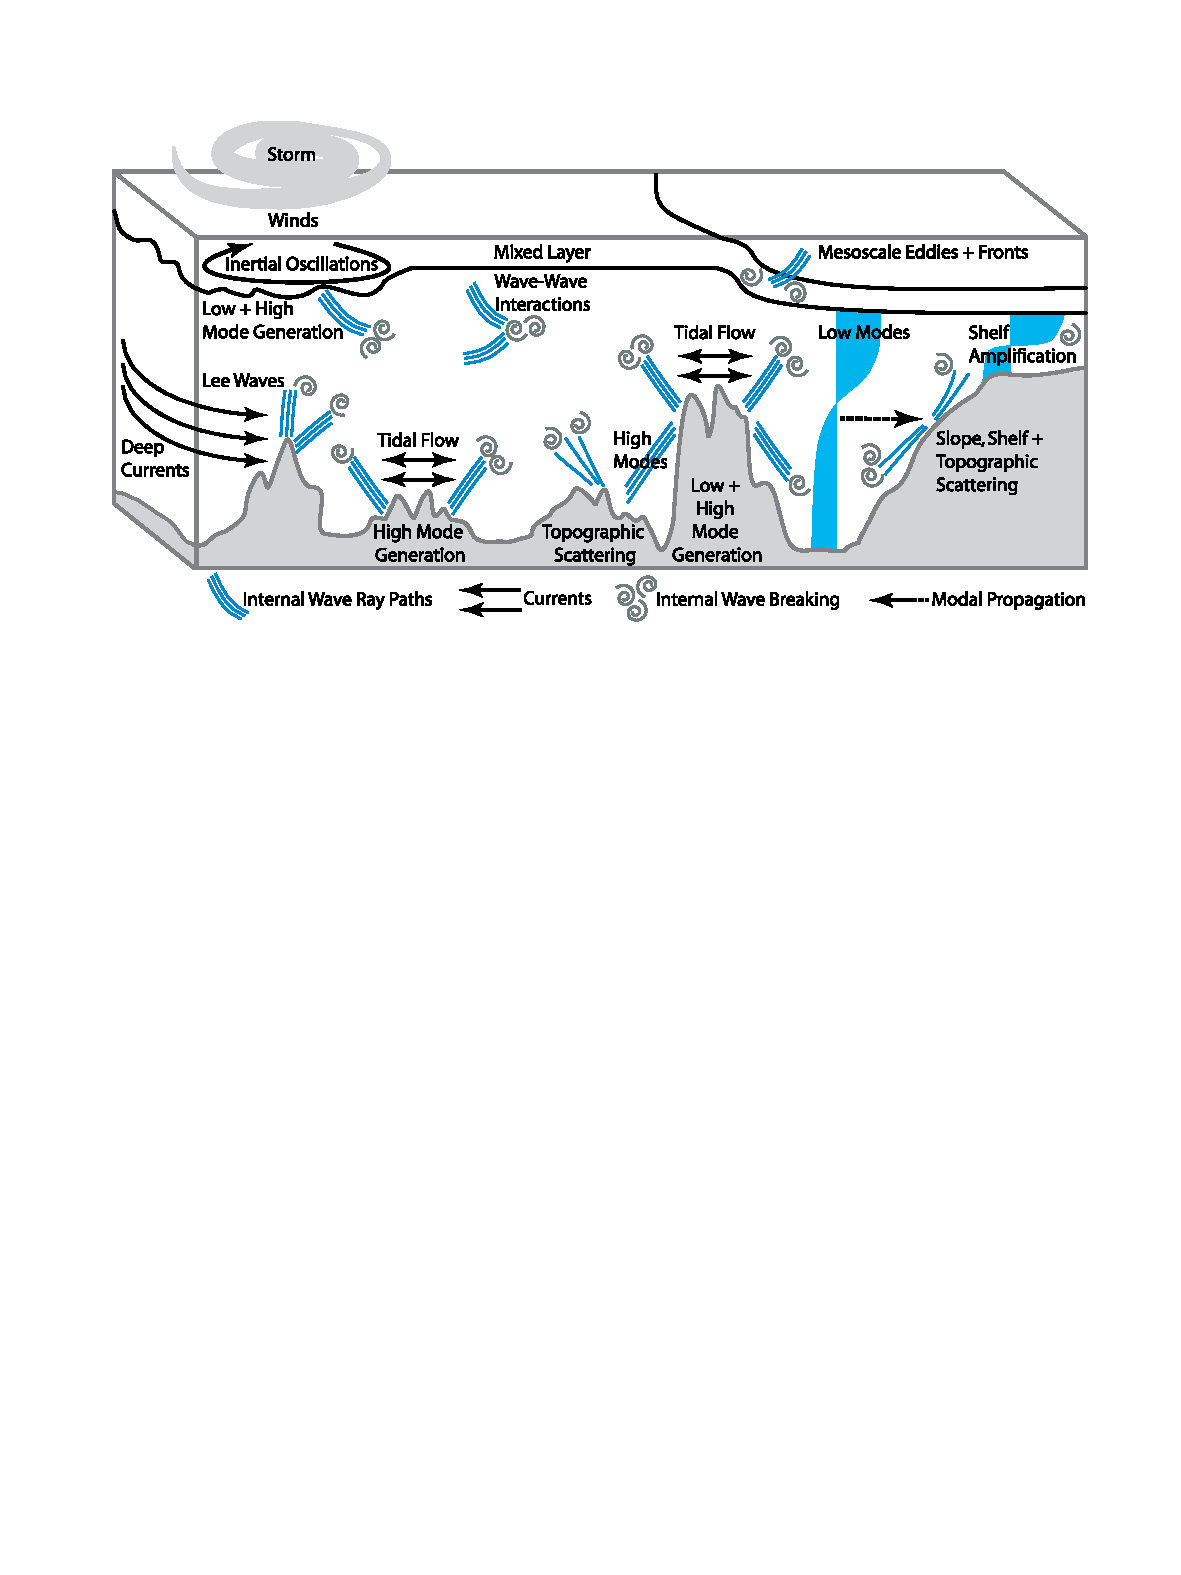
\includegraphics{figs/WaterMasses/MacKinnonEtAl17Fig1}
    \caption{Schematic of the zoo of ocean mixing processes \citep{MacKinnonEtAl17}.}
    \label{fig:MacKinnonEtAl17Fig1}  
  \end{center}
\end{figure}



%%% Local Variables:
%%% mode: latex
%%% TeX-master: t
%%% End:
